\documentclass[a4paper]{article}
\usepackage{longtable,float,hyperref,color,amsmath,amsxtra,amssymb,latexsym,amscd,amsthm,amsfonts,graphicx}
\usepackage{mathtools,tabu,enumitem,multirow,datetime}
\usepackage{tikz,graphicx}
\usetikzlibrary{shapes,arrows}
\usetikzlibrary{calc}
\usetikzlibrary{decorations.pathmorphing}
\numberwithin{equation}{section}
\allowdisplaybreaks
\usepackage{fancyhdr}
\pagestyle{fancy}
\fancyhf{}
\fancyhead[RE,LO]{\footnotesize \textsc \leftmark}
\cfoot{\thepage}
\renewcommand{\headrulewidth}{0.5pt}
\setcounter{tocdepth}{3}
\setcounter{secnumdepth}{3}
\usepackage{imakeidx}
\makeindex[columns=2, title=Alphabetical Index, 
           options= -s index.ist]
\title{\huge On Approximating Solution of One-Dimensional Elliptic Problems by Using Finite Volume Method}
\author{\textsc{Nguyen Quan Ba Hong}\footnote{Student ID. 1411103}\\
\textsc{Doan Tran Nguyen Tung}\footnote{Student ID. 1411352}\\
\textsc{Nguyen An Thinh}\footnote{Student ID. 1411289}\\
{\small Students at Faculty of Math and Computer Science}\\ 
{\small Ho Chi Minh University of Science, Vietnam} \\
{\small \texttt{email. nguyenquanbahong@gmail.com}}\\
{\small \texttt{email. dtrngtung@live.com}}\\
{\small \texttt{email. anthinh297@gmail.com}}\\
{\small \texttt{blog. \url{www.nguyenquanbahong.com}} 
\footnote{Copyright \copyright\ 2016-2017 by Nguyen Quan Ba Hong, Student at Ho Chi Minh University of Science, Vietnam. This document may be copied freely for the purposes of education and non-commercial research. Visit my site \texttt{\url{www.nguyenquanbahong.com}} to get more.}}}
\begin{document}
\maketitle
\begin{abstract}
This assignment aims at solving one-dimensional elliptic problems with Dirichlet boundary conditions numerically by using finite volume method on admissible meshes. 

We also implement one-dimensional elliptic problems with Dirichlet-Neumann boundary condition by \textsc{Matlab}  scripts, which is based on our teacher's \textsc{Matlab} scripts, at the end of this context.
\end{abstract}
\newpage
\thispagestyle{plain}
\begin{sloppypar}
\par\vspace*{.35\textheight}{\centering \textit{Dedicated to our beloved teachers, \textbf{Le Anh Ha} \\
and \textbf{Phung Thanh Tam}, who teach us \\
Finite Volume Method course.} \par}
\end{sloppypar}
\newpage
\tableofcontents
\newpage
\listoffigures
\newpage
\listoftables
\newpage
\section{A Finite Volume Method for the Dirichlet Problem}
\subsection{Formulation of Finite Volume Scheme}
We now consider the finite volume method for the academic Dirichlet problem\index{Dirichlet problem}, namely a second order differential operator\index{second order differential operator} without time dependent terms and with homogeneous Dirichlet boundary conditions\index{homogeneous Dirichlet boundary conditions}. 

Let $f$ be a given function from $\left(0,1\right)$ to $\mathbb{R}$, consider the following differential equation
\begin{align}
\label{1.1}
 - u''\left( x \right) &= f\left( x \right),x \in \left( {0,1} \right)\\
u\left( 0 \right) &= 0\\
u\left( 1 \right) &= 0 \label{1.3}
\end{align}
If $f \in C\left( {\left[ {0,1} \right],\mathbb{R}} \right)$, there exists a unique solution $u \in {C^2}\left( {\left[ {0,1} \right],\mathbb{R}} \right)$ to Problem \eqref{1.1}-\eqref{1.3}. In the sequel, this exact solution will be denoted by $u$. Note that the equation $-u''=f$ can be written in the conservative form\index{conservative form} $div\left( \mathbf{F} \right) = f$ with $\mathbf{F}=-u'$.

In order to compute a numerical approximation to the solution of this equation, let us define a mesh, denoted by $\mathcal{T}$, of the interval $\left(0,1\right)$ consisting of $N$ cells (or \textit{control volume})\index{control volume}, denoted by $K_i,\hspace{0.2cm}i=1,\ldots,N$, and $N$ points of $\left(0,1\right)$, denoted by $x_i,\hspace{0.2cm}\ldots,i=1,\ldots,N$, satisfying the following assumptions.\\
\\
\textbf{Definition 1.1 (Admissible one-dimensional mesh).} An admissible mesh\index{admissible mesh} of $\left(0,1\right)$, denoted by $\mathcal{T}$, is given by a family ${\left( {{K_i}} \right)_{i = 1, \ldots ,N}},\hspace{0.2cm}N \in {\mathbb{N}^*}$, such that ${K_i} = \left( {{x_{i - \frac{1}{2}}},{x_{i + \frac{1}{2}}}} \right)$, and a family ${\left( {{x_i}} \right)_{i = 0, \ldots ,N + 1}}$ such that
\begin{align}
{x_0} = {x_{\frac{1}{2}}} &= 0 < {x_1} < {x_{\frac{3}{2}}} <  \cdots  < {x_{i - \frac{1}{2}}} < {x_i} <\\
&< {x_{i + \frac{1}{2}}} <  \cdots  < {x_N} < {x_{N + \frac{1}{2}}} = {x_{N + 1}} = 1
\end{align}
One sets
\begin{align}
h_i = m\left( {{K_i}} \right) = {x_{i + \frac{1}{2}}} - {x_{i - \frac{1}{2}}},\hspace{0.2cm}i = 1, \ldots ,N
\end{align}
and therefore
\begin{align}
\sum\limits_{i = 1}^N {{h_i}}  = 1
\end{align}
and
\begin{align}
h_i^ -  &= {x_i} - {x_{i - \frac{1}{2}}},\hspace{0.2cm}i = 1, \ldots ,N\\
h_i^ +  &= {x_{i + \frac{1}{2}}} - {x_i},\hspace{0.2cm}i = 1, \ldots ,N\\
{h_{i + \frac{1}{2}}} &= {x_{i + 1}} - {x_i},\hspace{0.2cm}i = 0, \ldots ,N\\
size\left( \mathcal{T} \right) &= h = \max \left\{ {{h_i},\hspace{0.2cm}i = 1, \ldots ,N} \right\} \label{1.11}
\end{align}

The discrete unknowns are denoted by $u_i,\hspace{0.2cm}i=1,\ldots,N$, and are expected to be some approximation of $u$ in the cell $K_i$ (the discrete unknown $u_i$ can be viewed as an approximation of the mean value of $u$ over $K_i$, i.e.
\begin{align}
{u_i} = \frac{1}{{m\left( {{K_i}} \right)}}\int_{{K_i}} {u\left( x \right)dx}  = \frac{1}{{{x_{i + \frac{1}{2}}} - {x_{i - \frac{1}{2}}}}}\int_{{K_i}} {u\left( x \right)dx}  = \frac{1}{{{h_i}}}\int_{{K_i}} {u\left( x \right)dx} 
\end{align}
or of the value of $u\left(x_i\right)$, or of other values of $u$ in the control volume $K_i$, \ldots). The first equation \eqref{1.1} is integrated over each cell $K_i$ and yields
\begin{align}
\label{1.13}
 - {u'}\left( {{x_{i + \frac{1}{2}}}} \right) + {u'}\left( {{x_{i - \frac{1}{2}}}} \right) = \int_{{K_i}} {f\left( x \right)dx} ,\hspace{0.2cm} i = 1, \ldots ,N
\end{align}

A reasonable choice for the approximation of $- {u'}\left( {{x_{i + \frac{1}{2}}}} \right)$ (at least, for $i=1,\ldots,N-1$) seems to be the differential quotient\index{differential quotient}
\begin{align}
{F_{i + \frac{1}{2}}} =  - \frac{{{u_{i + 1}} - {u_i}}}{{{h_{i + \frac{1}{2}}}}}
\end{align}
This approximation is consistent in the sense that, if $u \in {C^2}\left( {\left[ {0,1} \right],\mathbb{R}} \right)$, then
\begin{align}
\label{1.15}
F_{i + \frac{1}{2}}^* &=  - \frac{{u\left( {{x_{i + 1}}} \right) - u\left( {{x_i}} \right)}}{{{h_{i + \frac{1}{2}}}}}\\
 &=  - {u'}\left( {{x_{i + \frac{1}{2}}}} \right) + O\left( h \right) \label{1.16}
\end{align}
where $\left| {O\left( h \right)} \right| \le Ch$ with $C \in {\mathbb{R}_ + }$ only depending on $u$.\\
\\
\textbf{Remark 1.2.} We can investigate \eqref{1.15}-\eqref{1.16} further as the following. Using the Taylor series expansion\index{Taylor series expansion} for $u\left(x_{i+1}\right)$ and $u\left(x_i\right)$ yields
\begin{align}
u\left( {{x_{i + 1}}} \right) &= u\left( {{x_{i + \frac{1}{2}}}} \right) + \left( {{x_{i + 1}} - {x_{i + \frac{1}{2}}}} \right)u'\left( {{x_{i + \frac{1}{2}}}} \right) \\
&+ \frac{1}{2}{\left( {{x_{i + 1}} - {x_{i + \frac{1}{2}}}} \right)^2}u''\left( {{x_{i + \frac{1}{2}}}} \right) + O\left( {{h^3}} \right)\\
u\left( {{x_i}} \right) &= u\left( {{x_{i + \frac{1}{2}}}} \right) + \left( {{x_i} - {x_{i + \frac{1}{2}}}} \right)u'\left( {{x_{i + \frac{1}{2}}}} \right) \\
&+ \frac{1}{2}{\left( {{x_i} - {x_{i + \frac{1}{2}}}} \right)^2}u''\left( {{x_{i + \frac{1}{2}}}} \right) + O\left( {{h^3}} \right)
\end{align}
Thus,
\begin{align}
u\left( {{x_{i + 1}}} \right) - u\left( {{x_i}} \right) &= \left( {{x_{i + 1}} - {x_i}} \right)u'\left( {{x_{i + \frac{1}{2}}}} \right)\\
& + \frac{1}{2}\left( {{{\left( {{x_{i + 1}} - {x_{i + \frac{1}{2}}}} \right)}^2} - {{\left( {{x_i} - {x_{i + \frac{1}{2}}}} \right)}^2}} \right)u''\left( {{x_{i + \frac{1}{2}}}} \right) + O\left( {{h^3}} \right)
\end{align}
We have two cases.
\begin{enumerate}
\item \textbf{Case 1.} \textit{$x_{i+\frac{1}{2}}$ is the midpoint of segment $\left[x_i,x_{i+1}\right]$,} then
\begin{align}
u'\left( {{x_{i + \frac{1}{2}}}} \right) = \frac{{u\left( {{x_{i + 1}}} \right) - u\left( {{x_i}} \right)}}{{{x_{i + 1}} - {x_i}}} + O\left( {{h^2}} \right)
\end{align}
\item \textbf{Case 2.} \textit{Otherwise,}
\begin{align}
u'\left( {{x_{i + \frac{1}{2}}}} \right) = \frac{{u\left( {{x_{i + 1}}} \right) - u\left( {{x_i}} \right)}}{{{x_{i + 1}} - {x_i}}} + O\left( h \right)
\end{align}
\end{enumerate}

Assume that $x_i$ is the center of $K_i$, i.e., ${x_i} = \frac{1}{2}{x_{i + \frac{1}{2}}} + \frac{1}{2}{x_{i - \frac{1}{2}}}$. Let $\widetilde{u}_i$ denote the mean value over $K_i$ of the exact solution $u$ to Problem \eqref{1.1}-\eqref{1.3}, i.e.
\begin{align}
{\widetilde u_i} = \frac{1}{{m\left( {{K_i}} \right)}}\int_{{K_i}} {u\left( x \right)dx}  = \frac{1}{{{x_{i + \frac{1}{2}}} - {x_{i - \frac{1}{2}}}}}\int_{{K_i}} {u\left( x \right)dx}  = \frac{1}{{{h_i}}}\int_{{x_{i - \frac{1}{2}}}}^{{x_{i + \frac{1}{2}}}} {u\left( x \right)dx} 
\end{align}
One may then remark that 
\begin{align}
\label{1.26}
\left| {{{\widetilde u}_i} - u\left( {{x_i}} \right)} \right| \le Ch_i^2
\end{align}
with some $C$ only depending on $u$.\\
\\
\textsc{Proof of \eqref{1.26}} Indeed,
\begin{align}
\left| {{{\widetilde u}_i} - u\left( {{x_i}} \right)} \right| &= \left| {\frac{1}{h_i}\int_{{x_{i - \frac{1}{2}}}}^{{x_{i + \frac{1}{2}}}} {u\left( x \right)dx}  - \frac{1}{h_i}\int_{{x_{i - \frac{1}{2}}}}^{{x_{i + \frac{1}{2}}}} {u\left( {{x_i}} \right)dx} } \right|\\
& = \left| {\frac{1}{h_i}\int_{{x_{i - \frac{1}{2}}}}^{{x_{i + \frac{1}{2}}}} {\left( {u\left( x \right) - u\left( {{x_i}} \right)} \right)dx} } \right|\\
& \le \frac{1}{h_i}\int_{{x_{i - \frac{1}{2}}}}^{{x_{i + \frac{1}{2}}}} {\left| {u\left( x \right) - u\left( {{x_i}} \right)} \right|dx} \label{1.29}
\end{align}

We now deal with the quantity ${u\left( x \right) - u\left( {{x_i}} \right)}$ with $x \in \left[ {{x_{i - \frac{1}{2}}},{x_{i + \frac{1}{2}}}} \right]$. To this end, since $x \in \left[ {{x_{i - \frac{1}{2}}},{x_{i + \frac{1}{2}}}} \right]$, we can represent $x$ as
\begin{align}
x = \left( {1 - t} \right){x_{i - \frac{1}{2}}} + t{x_{i + \frac{1}{2}}}\mbox{ for } t \in \left[ {0,1} \right]
\end{align}
Then, we have $dx = \left( {{x_{i + \frac{1}{2}}} - {x_{i - \frac{1}{2}}}} \right)dt = {h_i}dt$.

Using Taylor series expansion\index{Taylor series expansion} for $u\left( x \right)$ and $u\left( {{x_i}} \right)$ yields
\begin{align}
u\left( x \right) &= u\left( {\left( {1 - t} \right){x_{i - \frac{1}{2}}} + t{x_{i + \frac{1}{2}}}} \right)\\
 &= u\left( {{x_{i - \frac{1}{2}}}} \right) + t\left( {{x_{i + \frac{1}{2}}} - {x_{i - \frac{1}{2}}}} \right)u'\left( {{x_{i - \frac{1}{2}}}} \right) + O\left( {h_i^2} \right)\\
& = u\left( {{x_{i - \frac{1}{2}}}} \right) + t{h_i}u'\left( {{x_{i - \frac{1}{2}}}} \right) + O\left( {h_i^2} \right)\label{1.33}\\
u\left( {{x_i}} \right) &= u\left( {\frac{1}{2}{x_{i - \frac{1}{2}}} + \frac{1}{2}{x_{i + \frac{1}{2}}}} \right)\\
 &= u\left( {{x_{i - \frac{1}{2}}}} \right) + \frac{1}{2}\left( {{x_{i + \frac{1}{2}}} - {x_{i - \frac{1}{2}}}} \right)u'\left( {{x_{i - \frac{1}{2}}}} \right) + O\left( {h_i^2} \right)\\
 &= u\left( {{x_{i - \frac{1}{2}}}} \right) + \frac{1}{2}{h_i}u'\left( {{x_{i - \frac{1}{2}}}} \right) + O\left( {h_i^2} \right) \label{1.36}
\end{align}

Substituting \eqref{1.33} and \eqref{1.36} into \eqref{1.29} yields
\begin{align}
&\frac{1}{{{h_i}}}\int_{{x_{i - \frac{1}{2}}}}^{{x_{i + \frac{1}{2}}}} {\left| {u\left( x \right) - u\left( {{x_i}} \right)} \right|dx}  \\
&= \frac{1}{{{h_i}}}\int_0^1 {\left| {\left( {t - \frac{1}{2}} \right){h_i}u'\left( {{x_{i - \frac{1}{2}}}} \right) + O\left( {h_i^2} \right)} \right|{h_i}dt} \\
 &= \left. {\left( {\frac{1}{2}{h_i}u'\left( {{x_{i - \frac{1}{2}}}} \right){t^2} - \frac{1}{2}{h_i}u'\left( {{x_{i - \frac{1}{2}}}} \right)t} \right)} \right|_0^1 + O\left( {h_i^2} \right)\\
 &= O\left( {h_i^2} \right)
\end{align}
i.e., there exists a constant $C$ only depending on $u$ such that $\left| {{{\widetilde u}_i} - u\left( {{x_i}} \right)} \right| \le Ch_i^2$, as stated. \hfill $\square$\\

It follows easily that 
\begin{align}
\label{1.41}
\frac{{{{\widetilde u}_{i + 1}} - {{\widetilde u}_i}}}{{{h_{i + \frac{1}{2}}}}} = {u'}\left( {{x_{i + \frac{1}{2}}}} \right) + O\left( h \right),\hspace{0.2cm} i = 1, \ldots ,N - 1
\end{align}
\textsc{Proof 1 of \eqref{1.41}.} Indeed, applying the appendix \textit{``An Easy Change of Variables''} with 
\begin{align}
a &= {x_{i + \frac{1}{2}}},b = {x_{i + \frac{3}{2}}},c = {x_{i - \frac{1}{2}}},d = {x_{i + \frac{1}{2}}},f = u\\
S\left( x \right) &= \frac{{{x_{i + \frac{1}{2}}} - {x_{i - \frac{1}{2}}}}}{{{x_{i + \frac{3}{2}}} - {x_{i + \frac{1}{2}}}}}x + \frac{{{x_{i + \frac{3}{2}}}{x_{i - \frac{1}{2}}} - x_{i + \frac{1}{2}}^2}}{{{x_{i + \frac{3}{2}}} - {x_{i + \frac{1}{2}}}}}\\
 &= \frac{{{h_i}}}{{{h_{i + 1}}}}x + \frac{{{x_{i + \frac{3}{2}}}{x_{i - \frac{1}{2}}} - x_{i + \frac{1}{2}}^2}}{{{h_{i + 1}}}},\hspace{0.2cm}\forall x \in \left[ {{x_{i + \frac{1}{2}}},{x_{i + \frac{3}{2}}}} \right]\\
{S^{ - 1}}\left( y \right) &= \frac{{{x_{i + \frac{3}{2}}} - {x_{i + \frac{1}{2}}}}}{{{x_{i + \frac{1}{2}}} - {x_{i - \frac{1}{2}}}}}y + \frac{{{x_{i + \frac{1}{2}}}{x_{i + \frac{1}{2}}} - {x_{i + \frac{3}{2}}}{x_{i - \frac{1}{2}}}}}{{{x_{i + \frac{1}{2}}} - {x_{i - \frac{1}{2}}}}}\\
& = \frac{{{h_{i + 1}}}}{{{h_i}}}y + \frac{{x_{_{i + \frac{1}{2}}}^2 - {x_{i + \frac{3}{2}}}{x_{i - \frac{1}{2}}}}}{{{h_i}}},\hspace{0.2cm}\forall y \in \left[ {{x_{i - \frac{1}{2}}},{x_{i + \frac{1}{2}}}} \right]
\end{align}
yields
\begin{align}
{\widetilde u_{i + 1}} &= \frac{1}{{{h_{i + 1}}}}\int_{{x_{i + \frac{1}{2}}}}^{{x_{i + \frac{3}{2}}}} {u\left( x \right)dx} \\
 &= \frac{1}{{{h_{i + 1}}}}\int_{{x_{i - \frac{1}{2}}}}^{{x_{i + \frac{1}{2}}}} {u\left( {\frac{{{h_{i + 1}}}}{{{h_i}}}x + \frac{{x_{_{i + \frac{1}{2}}}^2 - {x_{i + \frac{3}{2}}}{x_{i - \frac{1}{2}}}}}{{{h_i}}}} \right)\frac{{{h_{i + 1}}}}{{{h_i}}}dx} \\
 &= \frac{1}{{{h_i}}}\int_{{x_{i - \frac{1}{2}}}}^{{x_{i + \frac{1}{2}}}} {u\left( {\frac{{{h_{i + 1}}}}{{{h_i}}}x + \frac{{x_{_{i + \frac{1}{2}}}^2 - {x_{i + \frac{3}{2}}}{x_{i - \frac{1}{2}}}}}{{{h_i}}}} \right)dx} 
\end{align}
Using Taylor series expansion\index{Taylor series expansion} as before, we obtain
\begin{align}
\label{1.50}
u\left( x \right) &= u\left( {\left( {1 - t} \right){x_{i - \frac{1}{2}}} + t{x_{i + \frac{1}{2}}}} \right),\mbox{ for } t \in \left[ {0,1} \right]\\
&= u\left( {{x_{i + \frac{1}{2}}}} \right) + \left( {t - 1} \right){h_i}u'\left( {{x_{i + \frac{1}{2}}}} \right) + O\left( {h_i^2} \right)
\end{align}
and
\begin{align}
&u\left( {\frac{{{h_{i + 1}}}}{{{h_i}}}x + \frac{{x_{_{i + \frac{1}{2}}}^2 - {x_{i + \frac{3}{2}}}{x_{i - \frac{1}{2}}}}}{{{h_i}}}} \right)\\
 &= u\left( {\frac{{{h_{i + 1}}}}{{{h_i}}}\left( {\left( {1 - t} \right){x_{i - \frac{1}{2}}} + t{x_{i + \frac{1}{2}}}} \right) + \frac{{x_{_{i + \frac{1}{2}}}^2 - {x_{i + \frac{3}{2}}}{x_{i - \frac{1}{2}}}}}{{{h_i}}}} \right),\mbox{ for } t \in \left[ {0,1} \right]\\
& = u\left( {{x_{i + \frac{1}{2}}}} \right) + {h_{i + 1}}u'\left( {{x_{i + \frac{1}{2}}}} \right)t + O\left( {h_{i + 1}^2} \right) \label{1.54}
\end{align}
where we have used
\begin{align}
&\frac{{{h_{i + 1}}}}{{{h_i}}}\left( {\left( {1 - t} \right){x_{i - \frac{1}{2}}} + t{x_{i + \frac{1}{2}}}} \right) + \frac{{x_{_{i + \frac{1}{2}}}^2 - {x_{i + \frac{3}{2}}}{x_{i - \frac{1}{2}}}}}{{{h_i}}} - {x_{i + \frac{1}{2}}}\\
 &= \frac{{{h_{i + 1}}}}{{{h_i}}}\left( {\left( {1 - t} \right){x_{i - \frac{1}{2}}} + t{x_{i + \frac{1}{2}}}} \right) - \frac{{\left( {{x_{i + \frac{3}{2}}} - {x_{i + \frac{1}{2}}}} \right){x_{i - \frac{1}{2}}}}}{{{x_{i + \frac{1}{2}}} - {x_{i - \frac{1}{2}}}}}\\
 &= \frac{{{h_{i + 1}}}}{{{h_i}}}\left( {{x_{i + \frac{1}{2}}} - {x_{i - \frac{1}{2}}}} \right)t\\
 &= {h_{i + 1}}t
\end{align}

Using \eqref{1.50}-\eqref{1.54} yields
\begin{align}
&\frac{{{{\widetilde u}_{i + 1}} - {{\widetilde u}_i}}}{{{h_{i + \frac{1}{2}}}}}\\
& = \frac{{\int_0^1 {\left( {{h_{i + 1}}u'\left( {{x_{i + \frac{1}{2}}}} \right)t - \left( {t - 1} \right){h_i}u'\left( {{x_{i + \frac{1}{2}}}} \right) + O\left( {h_{i + 1}^2} \right) + O\left( {h_i^2} \right)} \right){h_i}dt} }}{{{h_i}{h_{i + \frac{1}{2}}}}}\\
& = \frac{{\int_0^1 {\left( {\left( {{h_{i + 1}} - {h_i}} \right)u'\left( {{x_{i + \frac{1}{2}}}} \right)t + {h_i}u'\left( {{x_{i + \frac{1}{2}}}} \right) + O\left( {h_{i + 1}^2 + h_i^2} \right)} \right)dt} }}{{{h_{i + \frac{1}{2}}}}}\\
& = \frac{{\left. {\left( {\left( {{h_{i + 1}} - {h_i}} \right)u'\left( {{x_{i + \frac{1}{2}}}} \right)\frac{{{t^2}}}{2} + {h_i}u'\left( {{x_{i + \frac{1}{2}}}} \right)t} \right)} \right|_0^1 + O\left( {h_{i + 1}^2 + h_i^2} \right)}}{{{h_{i + \frac{1}{2}}}}}\\
& = \frac{{{h_{i + 1}} + {h_i}}}{{2{h_{i + \frac{1}{2}}}}}u'\left( {{x_{i + \frac{1}{2}}}} \right) + \frac{1}{{{h_{i + \frac{1}{2}}}}}O\left( {h_{i + 1}^2 + h_i^2} \right)\\
& = u'\left( {{x_{i + \frac{1}{2}}}} \right) + O\left( h \right),\hspace{0.2cm} i=1,\ldots,N-1
\end{align}
where the last equality is deduced from
\begin{align}
{h_{i + 1}} + {h_i} &= {x_{i + \frac{3}{2}}} - {x_{i + \frac{1}{2}}} + {x_{i + \frac{1}{2}}} - {x_{i - \frac{1}{2}}}\\
 &= {x_{i + \frac{3}{2}}} + {x_{i + \frac{1}{2}}} - \left( {{x_{i + \frac{1}{2}}} + {x_{i - \frac{1}{2}}}} \right)\\
 &= 2{x_{i + 1}} - 2{x_i}\\
 &= 2{h_{i + \frac{1}{2}}},\hspace{0.2cm} i = 1, \ldots ,N-1 \label{1.68}
\end{align}
and
\begin{align}
\frac{{h_{i + 1}^2 + h_i^2}}{{{h_{i + \frac{1}{2}}}}} &= \frac{{2\left( {h_{i + 1}^2 + h_i^2} \right)}}{{{h_{i + 1}} + {h_i}}}\mbox{ by \eqref{1.68}}\\
 &\le \frac{{2{{\left( {{h_{i + 1}} + {h_i}} \right)}^2}}}{{{h_{i + 1}} + {h_i}}}\\
 &= 2\left( {{h_{i + 1}} + {h_i}} \right)\\
 &= O\left( h \right),\hspace{0.2cm} i = 1, \ldots ,N-1\mbox{ by \eqref{1.11}}
\end{align}
So \eqref{1.41} is proved. \hfill $\square$\\
\\
\textsc{Proof 2 of \eqref{1.41}.} Instead of using a change of variables\index{change of variables}, we can approach more directly by looking at the common point $x_{i+\frac{1}{2}}$ of $K_i$ and $K_{i+1}$ as follows.

Using Taylor series expansion\index{Taylor series expansion} for $\widetilde{u}_i$ and $\widetilde{u}_{i+1}$ yields
\begin{align}
{\widetilde u_i} &= \frac{1}{{{h_i}}}\int_{{x_{i - \frac{1}{2}}}}^{{x_{i + \frac{1}{2}}}} {u\left( x \right)dx} \\
 &= \frac{1}{{{h_i}}}\int_0^1 {u\left( {\left( {1 - t} \right){x_{i - \frac{1}{2}}} + t{x_{i + \frac{1}{2}}}} \right){h_i}dt} \\
 &= \int_0^1 {\left( {u\left( {{x_{i + \frac{1}{2}}}} \right) + \left( {t - 1} \right){h_i}u'\left( {{x_{i + \frac{1}{2}}}} \right) + O\left( {h_i^2} \right)} \right)dt} \\
{\widetilde u_{i + 1}} &= \frac{1}{{{h_{i + 1}}}}\int_{{x_{i + \frac{1}{2}}}}^{{x_{i + \frac{3}{2}}}} {u\left( x \right)dx} \\
 &= \frac{1}{{{h_{i + 1}}}}\int_0^1 {u\left( {\left( {1 - t} \right){x_{i + \frac{1}{2}}} + t{x_{i + \frac{3}{2}}}} \right){h_{i + 1}}dt} \\
 &= \int_0^1 {\left( {u\left( {{x_{i + \frac{1}{2}}}} \right) + t{h_{i + 1}}u'\left( {{x_{i + \frac{1}{2}}}} \right) + O\left( {h_{i + 1}^2} \right)} \right)dt} 
\end{align}
then
\begin{align}
&\frac{{{{\widetilde u}_{i + 1}} - {{\widetilde u}_i}}}{{{h_{i + \frac{1}{2}}}}} \\
&= \frac{{\int_0^1 {\left( {\left( {{h_{i + 1}} - {h_i}} \right)u'\left( {{x_{i + \frac{1}{2}}}} \right)t + {h_i}u'\left( {{x_{i + \frac{1}{2}}}} \right) + O\left( {h_i^2} \right) + O\left( {h_{i + 1}^2} \right)} \right)dt} }}{{{h_{i + \frac{1}{2}}}}}\\
& = \frac{{\left. {\left( {\left( {{h_{i + 1}} - {h_i}} \right)u'\left( {{x_{i + \frac{1}{2}}}} \right)\frac{{{t^2}}}{2} + {h_i}u'\left( {{x_{i + \frac{1}{2}}}} \right)t} \right)} \right|_0^1 + O\left( {h_i^2 + h_{i + 1}^2} \right)}}{{{h_{i + \frac{1}{2}}}}}\\
& = \frac{{\frac{1}{2}\left( {{h_{i + 1}} - {h_i}} \right)u'\left( {{x_{i + \frac{1}{2}}}} \right) + {h_i}u'\left( {{x_{i + \frac{1}{2}}}} \right) + O\left( {h_i^2 + h_{i + 1}^2} \right)}}{{{h_{i + \frac{1}{2}}}}}\\
& = \frac{{{h_{i + 1}} + {h_i}}}{{2{h_{i + \frac{1}{2}}}}}u'\left( {{x_{i + \frac{1}{2}}}} \right) + \frac{1}{{{h_{i + \frac{1}{2}}}}}O\left( {h_i^2 + h_{i + 1}^2} \right)\\
& = u'\left( {{x_{i + \frac{1}{2}}}} \right) + O\left( h \right),\hspace{0.2cm} i = 1, \ldots ,N-1
\end{align}
where the last equality is handled as in the first proof. \hfill $\square$\\

Hence the approximation of the flux\index{flux} is also consistent if the discrete unknowns $u_i,\hspace{0.2cm}i=1,\ldots,N$, are viewed as approximations of the mean value of $u$ in the control volumes.

The Dirichlet boundary conditions\index{Dirichlet boundary conditions} are taken into account by using the values imposed at the boundaries to compute the fluxes on these boundaries. Taking these boundary conditions into consideration and setting 
\begin{align}
{f_i} = \frac{1}{{{h_i}}}\int_{{K_i}} {f\left( x \right)dx} ,\hspace{0.2cm} i = 1, \ldots ,N
\end{align}
(in actual computation, an approximation of $f_i$ by numerical integration can be used), the finite volume scheme\index{finite volume scheme} for problem \eqref{1.1}-\eqref{1.3} writes
\begin{align}
\label{1.86}
{F_{i + \frac{1}{2}}} - {F_{i - \frac{1}{2}}} &= {h_i}{f_i},\hspace{0.2cm}i = 1, \ldots ,N\\
{F_{i + \frac{1}{2}}} &=  - \frac{{{u_{i + 1}} - {u_i}}}{{{h_{i + \frac{1}{2}}}}},\hspace{0.2cm}i = 1, \ldots ,N - 1\label{1.87}\\
{F_{\frac{1}{2}}} &=  - \frac{{{u_1}}}{{{h_{\frac{1}{2}}}}}\label{1.88}\\
{F_{N + \frac{1}{2}}} &= \frac{{{u_N}}}{{{h_{N + \frac{1}{2}}}}} \label{1.89}
\end{align}

Note that \eqref{1.87}-\eqref{1.89} may also be written
\begin{align}
{F_{i + \frac{1}{2}}} =  - \frac{{{u_{i + 1}} - {u_i}}}{{{h_{i + \frac{1}{2}}}}},\hspace{0.2cm}i = 0, \ldots ,N
\end{align}
setting
\begin{align}
\label{1.91}
{u_0} = {u_{N + 1}} = 0
\end{align}

The numerical scheme \eqref{1.86}-\eqref{1.89} may be written under the following matrix form
\begin{align}
\label{1.92}
AU=b
\end{align}
where $U = {\left( {{u_1}, \ldots ,{u_N}} \right)^t},b = {\left( {{b_1}, \ldots ,{b_N}} \right)^t}$ with \eqref{1.91} and with $A$ and $b$ defined by
\begin{align}
{\left( {AU} \right)_i} &= \frac{1}{{{h_i}}}\left( { - \frac{{{u_{i + 1}} - {u_i}}}{{{h_{i + \frac{1}{2}}}}} + \frac{{{u_i} - {u_{i - 1}}}}{{{h_{i - \frac{1}{2}}}}}} \right),\hspace{0.2cm}i = 1, \ldots ,N\\
{b_i} &= \frac{1}{{{h_i}}}\int_{{K_i}} {f\left( x \right)dx} ,\hspace{0.2cm}i = 1, \ldots ,N \label{1.94}
\end{align}
More explicitly, the matrix $A$ is given by
\begin{align}
\label{1.95}
A = \left[ {\begin{array}{*{20}{c}}
{\frac{1}{{{h_1}}}\left( {\frac{1}{{{h_{\frac{1}{2}}}}} + \frac{1}{{{h_{\frac{3}{2}}}}}} \right)}&{ - \frac{1}{{{h_1}{h_{\frac{3}{2}}}}}}&{}&{}\\
{ - \frac{1}{{{h_{\frac{3}{2}}}{h_2}}}}&{\frac{1}{{{h_2}}}\left( {\frac{1}{{{h_{\frac{3}{2}}}}} + \frac{1}{{{h_{\frac{5}{2}}}}}} \right)}&{ - \frac{1}{{{h_2}{h_{\frac{5}{2}}}}}}&{}\\
{}& \ddots & \ddots & \ddots \\
{}&{}&{ - \frac{1}{{{h_{N - \frac{1}{2}}}{h_N}}}}&{\frac{1}{{{h_N}}}\left( {\frac{1}{{{h_{N - \frac{1}{2}}}}} + \frac{1}{{{h_{N + \frac{1}{2}}}}}} \right)}
\end{array}} \right]
\end{align}

Put, for all $i=1,\ldots,N$,
\begin{align}
{\alpha _i} &=  - \frac{1}{{{h_{i - \frac{1}{2}}}{h_i}}}\\
{\beta _i} &= \frac{1}{{{h_i}}}\left( {\frac{1}{{{h_{i - \frac{1}{2}}}}} + \frac{1}{{{h_{i + \frac{1}{2}}}}}} \right)\\
{\gamma _i} &=  - \frac{1}{{{h_i}{h_{i + \frac{1}{2}}}}}
\end{align}
we get
\begin{align}
{\alpha _i}{u_{i - 1}} + {\beta _i}{u_i} + {\gamma _i}{u_{i + 1}} = {b_i},\hspace{0.2cm} i = 1, \ldots ,N
\end{align}

Combining with the boundary conditions, we get the scheme for the cell-centered finite volume method\index{cell-centered finite volume method}
\begin{align}
\left\{ {\begin{array}{*{20}{c}}
{{\alpha _i}{u_{i - 1}} + {\beta _i}{u_i} + {\gamma _i}{u_{i + 1}} = {b_i},i = 1, \ldots ,N}\\
{{u_0} = {u_{N + 1}} = 0}
\end{array}} \right.
\end{align}
With these notations, \eqref{1.95} can be rewritten as
\begin{align}
A = \left[ {\begin{array}{*{20}{c}}
{{\beta _1}}&{{\gamma _1}}&{}&{}&{}&{}\\
{{\alpha _2}}&{{\beta _2}}&{{\gamma _2}}&{}&{}&{}\\
{}&{{\alpha _3}}&{{\beta _3}}&{{\gamma _3}}&{}&{}\\
{}&{}& \ddots & \ddots & \ddots &{}\\
{}&{}&{}&{{\alpha _{N - 1}}}&{{\beta _{N - 1}}}&{{\gamma _N}}\\
{}&{}&{}&{}&{{\alpha _N}}&{{\beta _N}}
\end{array}} \right]
\end{align}
The matrix $A$ is tridiagonal\index{tridiagonal matrices} and symmetric positive definite\index{symmetric positive definite matrices}.\\
\\
\textbf{Remark 1.3} There are other finite volume schemes\index{finite volume schemes} for problem \eqref{1.1}-\eqref{1.3}.
\begin{enumerate}
\item For instance, it is possible, in Definition 2.1, to take $x_1\ge 0,x_N\le 1$ and, for the definition of the scheme (that is \eqref{1.94}-\eqref{1.89}), to write \eqref{1.94} only for $i=2,\ldots,N-1$ and to replace \eqref{1.88} and \eqref{1.89} by $u_1=u_N=0$ (note that \eqref{1.87} does not change). For this so-called ``modified finite volume'' scheme\index{modified finite volume scheme}, it is also possible to obtain an error estimate\index{error estimate} as for the scheme \eqref{1.94}-\eqref{1.89} (see Remark 2.3). Note that, with this scheme, the union of all control volumes for which the ``conservation law''\index{conservation law} is written is slightly different from $\left[0,1\right]$ (namely $\left[ {{x_{\frac{3}{2}}},{x_{N - \frac{1}{2}}}} \right] \ne \left[ {0,1} \right]$).
\item Another possibility is to take (primary) unknowns associated to the boundaries of the control volumes. We shall not consider this case here.
\end{enumerate}
\subsection{Comparison with a Finite Difference Scheme}
With the same notations as in Section 1.1, consider that $u_i$ is now an approximation of $u\left(x_i\right)$. It is interesting to notice that the expression
\begin{align}
\frac{1}{{{h_i}}}\left( { - \frac{{{u_{i + 1}} - {u_i}}}{{{h_{i + \frac{1}{2}}}}} + \frac{{{u_i} - {u_{i - 1}}}}{{{h_{i - \frac{1}{2}}}}}} \right)
\end{align}
is not a consistent approximation of $-u''\left(x_i\right)$ in the finite difference sense\index{finite difference sense}, that is the error made by replacing the derivative by a difference quotient\index{difference quotient} does not tend to 0 as $h$ tends to 0. Indeed, let $\overline U  = {\left( {u\left( {{x_1}} \right), \ldots ,u\left( {{x_N}} \right)} \right)^t}$; with the notations of \eqref{1.92}-\eqref{1.94}, the truncation error\index{truncation error} may be defined as
\begin{align}
r = A\overline U  - b
\end{align}
with $r = {\left( {{r_1}, \ldots ,{r_N}} \right)^t}$. Note that for $f$ regular enough, which is assumed in the sequel, ${b_i} = f\left( {{x_i}} \right) + O\left( h \right)$. More explicitly, since ${x_i} \in \left( {{x_{i - \frac{1}{2}}},{x_{i + \frac{1}{2}}}} \right)$, there exists a constant $t_0$ such that ${x_i} = \left( {1 - {t_0}} \right){x_{i - \frac{1}{2}}} + {t_0}{x_{i + \frac{1}{2}}}$. Then, as usual, we have
\begin{align}
{b_i} &= \frac{1}{{{h_i}}}\int_{{K_i}} {f\left( x \right)dx} \\
& = \frac{1}{{{h_i}}}\int_{{x_{i - \frac{1}{2}}}}^{{x_{i + \frac{1}{2}}}} {f\left( x \right)dx} \\
& = \frac{1}{{{h_i}}}\int_0^1 {f\left( {\left( {1 - t} \right){x_{i - \frac{1}{2}}} + t{x_{i + \frac{1}{2}}}} \right){h_i}dt} \\
 &= \int_0^1 {\left( {f\left( {{x_i}} \right) + \left( {t - {t_0}} \right){h_i}f'\left( {{x_i}} \right) + O\left( {h_i^2} \right)} \right)dt} \\
 &= f\left( {{x_i}} \right) + \left( {\frac{1}{2} - {t_0}} \right){h_i}f'\left( {{x_i}} \right) + O\left( {h_i^2} \right)
\end{align}
i.e., ${b_i} = f\left( {{x_i}} \right) + O\left( h \right)$. In addition, if $t_0=\frac{1}{2}$, i.e., $x_i$ is center of $K_i$, we have ${b_i} = f\left( {{x_i}} \right) + O\left( h^2 \right)$.

An estimate of $r$ is obtained by using Taylor's expansion
\begin{align}
u\left( {{x_{i + 1}}} \right) &= u\left( {{x_i}} \right) + {h_{i + \frac{1}{2}}}u'\left( {{x_i}} \right) + \frac{1}{2}h_{i + \frac{1}{2}}^2u''\left( {{x_i}} \right) + \frac{1}{6}h_{i + \frac{1}{2}}^3u'''\left( {{\xi _i}} \right)\\
u\left( {{x_{i - 1}}} \right) &= u\left( {{x_i}} \right) - {h_{i - \frac{1}{2}}}u'\left( {{x_i}} \right) + \frac{1}{2}h_{i - \frac{1}{2}}^2u''\left( {{x_i}} \right) - \frac{1}{6}h_{i - \frac{1}{2}}^3u'''\left( {{\eta _i}} \right)
\end{align}
for some ${\xi _i} \in \left( {{x_i},{x_{i + 1}}} \right)$ and ${\eta _i} \in \left( {{x_{i - 1}},{x_i}} \right)$, which yields
\begin{align}
{r_i} &= {\left( {A\overline U } \right)_i} - {b_i}\\
 &= \frac{1}{{{h_i}}}\left( { - \frac{{u\left( {{x_{i + 1}}} \right) - u\left( {{x_i}} \right)}}{{{h_{i + \frac{1}{2}}}}} + \frac{{u\left( {{x_i}} \right) - u\left( {{x_{i - 1}}} \right)}}{{{h_{i - \frac{1}{2}}}}}} \right) - f\left( {{x_i}} \right) + O\left( h \right)\\
& = \frac{1}{{{h_i}}}\left( \begin{array}{l}
 - u'\left( {{x_i}} \right) - \frac{1}{2}{h_{i + \frac{1}{2}}}u''\left( {{x_i}} \right) + O\left( {h_{i + \frac{1}{2}}^2} \right)\\
 + u'\left( {{x_i}} \right) - \frac{1}{2}{h_{i - \frac{1}{2}}}u''\left( {{x_i}} \right) + O\left( {h_{i - \frac{1}{2}}^2} \right)
\end{array} \right) - f\left( {{x_i}} \right) + O\left( h \right)\\
 &=  - \frac{{{h_{i - \frac{1}{2}}} + {h_{i + \frac{1}{2}}}}}{{2{h_i}}}u''\left( {{x_i}} \right) + \frac{1}{{{h_i}}}O\left( {h_{i - \frac{1}{2}}^2 + h_{i + \frac{1}{2}}^2} \right) + u''\left( {{x_i}} \right) + O\left( h \right) \label{1.114}
\end{align}
for $i = 1, \ldots ,N$, which does not, in general tend to 0 as $h$ tends to 0 (except in particular case, for instance, $\mathcal{T}$ is a uniform admissible mesh\index{uniform admissible mesh} and $x_i$ is the center of $K_i$, then ${h_{i + \frac{1}{2}}} = {h_j},i = 0, \ldots ,N;j = 1, \ldots ,N$ and \eqref{1.114} becomes ${r_i} = O\left( h \right)$) as may be seen on the simple following example.\\
\\
\textbf{Example 1.4.} Let $f \equiv 1$ and consider a mesh of $\left(0,1\right)$, in the sense of Definition 2.1, satisfying $h_i=h$ for even $i$, $h_i=\frac{h}{2}$ for odd $i$ and ${x_i} = \frac{1}{2}{x_{i - \frac{1}{2}}} + \frac{1}{2}{x_{i + \frac{1}{2}}}$ for $i=1,\ldots,N$. An easy computation shows that the truncation error $r$ is 
\begin{align}
\label{1.115}
{r_i} = \left\{ {\begin{array}{*{20}{c}}
{ - \frac{1}{4},\mbox{ for even } i}\\
{\frac{1}{2},\mbox{ for odd } i}
\end{array}} \right.
\end{align}
\textsc{Proof of \eqref{1.115}.} With $f=1$, we have $u\left( x \right) = \frac{1}{2}x\left( {1 - x} \right),\hspace{0.2cm}\forall x \in \left( {0,1} \right)$. It is easily to find out
\begin{align}
{x_{2k}} &= \frac{3}{2}kh - \frac{h}{2}\\
{x_{2k + \frac{1}{2}}} &= \frac{3}{2}kh\\
{x_{2k + 1}} &= \frac{3}{2}kh + \frac{h}{4}\\
{x_{2k + 1 + \frac{1}{2}}} &= \frac{3}{2}kh + \frac{h}{2}
\end{align}
Therefore,
\begin{align}
{r_{2k}} &= \frac{1}{{{h_{2k}}}}\left( { - \frac{{u\left( {{x_{2k + 1}}} \right) - u\left( {{x_{2k}}} \right)}}{{{x_{2k + 1}} - {x_{2k}}}} + \frac{{u\left( {{x_{2k}}} \right) - u\left( {{x_{2k - 1}}} \right)}}{{{x_{2k}} - {x_{2k - 1}}}}} \right)\\
 &- \frac{1}{{{h_{2k}}}}\int_{{K_{2k}}} {f\left( x \right)dx} \\
 &= \frac{1}{h}\left( \begin{array}{l}
 - \dfrac{{u\left( {\frac{3}{2}kh + \frac{h}{4}} \right) - u\left( {\frac{3}{2}kh - \frac{h}{2}} \right)}}{{\frac{3}{2}kh + \frac{h}{4} - \left( {\frac{3}{2}kh - \frac{h}{2}} \right)}}\\
 + \dfrac{{u\left( {\frac{3}{2}kh - \frac{h}{2}} \right) - u\left( {\frac{3}{2}kh - \frac{{5h}}{4}} \right)}}{{\frac{3}{2}kh - \frac{h}{2} - \left( {\frac{3}{2}kh - \frac{{5h}}{4}} \right)}}
\end{array} \right) - 1\\
& = \frac{1}{h}\left( \begin{array}{l}
 - \dfrac{{u\left( {\frac{3}{2}kh + \frac{h}{4}} \right) - u\left( {\frac{3}{2}kh - \frac{h}{2}} \right)}}{{\frac{{3h}}{4}}}\\
 + \dfrac{{u\left( {\frac{3}{2}kh - \frac{h}{2}} \right) - u\left( {\frac{3}{2}kh - \frac{{5h}}{4}} \right)}}{{\frac{{3h}}{4}}}
\end{array} \right) - 1\\
 &=  - \frac{1}{4} \label{1.124}
\end{align}
and
\begin{align}
{r_{2k + 1}} &= \frac{1}{{{h_{2k + 1}}}}\left( { - \frac{{u\left( {{x_{2k + 2}}} \right) - u\left( {{x_{2k + 1}}} \right)}}{{{h_{2k + 1 + \frac{1}{2}}}}} + \frac{{u\left( {{x_{2k + 1}}} \right) - u\left( {{x_{2k}}} \right)}}{{{h_{2k + \frac{1}{2}}}}}} \right)\\
& - \frac{1}{{{h_{2k + 1}}}}\int_{{K_{2k + 1}}} {f\left( x \right)dx} \\
& = \frac{2}{h}\left( \begin{array}{l}
 - \dfrac{{u\left( {\frac{3}{2}kh + h} \right) - u\left( {\frac{3}{2}kh + \frac{h}{4}} \right)}}{{{x_{2k + 2}} - {x_{2k + 1}}}}\\
 + \dfrac{{u\left( {\frac{3}{2}kh + \frac{h}{4}} \right) - u\left( {\frac{3}{2}kh - \frac{h}{2}} \right)}}{{{x_{2k + 1}} - {x_{2k}}}}
\end{array} \right) - 1\\
& = \frac{2}{h}\left( \begin{array}{l}
 - \dfrac{{u\left( {\frac{3}{2}kh + h} \right) - u\left( {\frac{3}{2}kh + \frac{h}{4}} \right)}}{{\frac{3}{2}kh + h - \left( {\frac{3}{2}kh + \frac{h}{4}} \right)}}\\
 + \dfrac{{u\left( {\frac{3}{2}kh + \frac{h}{4}} \right) - u\left( {\frac{3}{2}kh - \frac{h}{2}} \right)}}{{\frac{3}{2}kh + \frac{h}{4} - \left( {\frac{3}{2}kh - \frac{h}{2}} \right)}}
\end{array} \right) - 1\\
& = \frac{2}{h}\left( \begin{array}{l}
 - \dfrac{{u\left( {\frac{3}{2}kh + h} \right) - u\left( {\frac{3}{2}kh + \frac{h}{4}} \right)}}{{\frac{{3h}}{4}}}\\
 + \dfrac{{u\left( {\frac{3}{2}kh + \frac{h}{4}} \right) - u\left( {\frac{3}{2}kh - \frac{h}{2}} \right)}}{{\frac{{3h}}{4}}}
\end{array} \right) - 1\\
 &= \frac{1}{2} \label{1.130}
\end{align}
where \eqref{1.124} and \eqref{1.130} can be computed easily by hand, or by using the following short \textsc{Matlab} code.
\begin{verbatim}
function u = u(x)
u = 1/2*x*(1-x);
\end{verbatim} 
and 
\begin{verbatim}
% Example 2.3.
syms h k;
r_even = 1/h*(-(u(3/2*k*h+h/4)-u(3/2*k*h-h/2))/(3/4*h)+ ...
    (u(3/2*k*h-h/2)-u(3/2*k*h-5/4*h))/(3/4*h))-1;
simplify(r_even)
r_odd= 2/h*(-(u(3/2*k*h+h)-u(3/2*k*h+h/4))/(3/4*h)+ ...
    (u(3/2*k*h+h/4)-u(3/2*k*h-h/2))/(3/4*h))-1;
simplify(r_odd)
\end{verbatim}
Hence, $\sup \left\{ {\left| {{r_i}} \right|,i = 1, \ldots ,N} \right\}\not  \to 0$ as $h\to 0$.

Therefore, the scheme obtained from \eqref{1.94}-\eqref{1.89} is not consistent in the finite difference sense\index{finite difference sense}, even though it is consistent in the finite volume sense, that is, the numerical approximation of the fluxes is conservative and the truncation error on the fluxes\index{truncation error on fluxes} tends to 0 as $h$ tends to 0.

If, for instance, $x_i$ is the center of $K_i$, for $i=1,\ldots,N$, it is well known that for problem \eqref{1.1}-\eqref{1.3}, the consistent finite difference scheme\index{consistent finite difference scheme} would be, omitting boundary conditions,
\begin{align}
\label{1.131}
\dfrac{4}{{2{h_i} + {h_{i - 1}} + {h_{i + 1}}}}\left( { - \frac{{{u_{i + 1}} - {u_i}}}{{{h_{i + \frac{1}{2}}}}} + \frac{{{u_i} - {u_{i - 1}}}}{{{h_{i - \frac{1}{2}}}}}} \right) = f\left( {{x_i}} \right),\hspace{0.2cm} i = 2, \ldots ,N - 1
\end{align}
\textbf{Remark 1.5.} Assume that $x_i$ is, for $i=1,\ldots,N$, the center of $K_i$ and that the discrete unknown $u_i$ of the finite volume scheme\index{finite volume scheme} is considered as an approximation of the mean value $\widetilde{u}_i$ of $u$ over $K_i$. Note that
\begin{align}
{\widetilde u_i} &= \frac{1}{{{h_i}}}\int_{{x_{i - \frac{1}{2}}}}^{{x_{i + \frac{1}{2}}}} {u\left( x \right)dx} \\
& = \int_0^1 {u\left( {\left( {1 - t} \right){x_{i - \frac{1}{2}}} + t{x_{i + \frac{1}{2}}}} \right)dt} \\
& = \int_0^1 {\left( {u\left( {{x_i}} \right) + \left( {t - \frac{1}{2}} \right){h_i}u'\left( {{x_i}} \right) + \frac{1}{2}{{\left( {t - \frac{1}{2}} \right)}^2}h_i^2u''\left( {{x_i}} \right) + O\left( {h_i^3} \right)} \right)dt} \\
& = u\left( {{x_i}} \right) + \frac{{h_i^2}}{{24}}u''\left( {{x_i}} \right) + O\left( {{h^3}} \right) \label{1.135}
\end{align} 
if $u \in {C^3}\left( {\left[ {0,1} \right],\mathbb{R}} \right)$ instead of $u\left(x_i\right)$, then again, the finite volume scheme\index{finite volume scheme}, considered once more as a finite difference scheme, is not consistent in the finite difference sense\index{finite difference sense}. Indeed, let $\widetilde R = A\widetilde U - b$, with $\widetilde U = {\left( {{{\widetilde u}_1}, \ldots ,{{\widetilde u}_N}} \right)^t}$ , and $\widetilde R = {\left( {{{\widetilde R}_1}, \ldots ,{{\widetilde R}_N}} \right)^t}$, then, in general, $\widetilde{R}_i$ does not go to 0 as $h$ goes to 0. In fact, it will be shown later that the finite volume scheme\index{finite volume scheme}, when seen as a finite difference scheme\index{finite difference scheme}, is consistent in the finite difference sense\index{finite difference sense} if $u_i$ is considered as an approximation of $u\left( {{x_i}} \right) - \frac{{h_i^2}}{8}{u''}\left( {{x_i}} \right)$. This is the idea upon which the first proof of convergence by Forsyth and Sammon in 1988 is based.

In the case of Problem \eqref{1.1}-\eqref{1.3}, both the finite volume and finite difference schemes are convergent. The finite difference scheme\index{finite difference scheme} \eqref{1.131} is convergent since it is stable, in the sense that ${\left\| X \right\|_\infty } \le C{\left\| {AX} \right\|_\infty }$, for all $X\in \mathbb{R}^N$, where $C$ is a constant and ${\left\| X \right\|_\infty } = \sup \left( {\left| {{X_1}} \right|, \ldots ,\left| {{X_N}} \right|} \right)$, $X = {\left( {{X_1}, \ldots ,{X_N}} \right)^t}$, and consistent in the usual finite difference sense\index{finite difference sense}. Since $A\left( {\overline U  - U} \right) = R$, the stability property\index{stability property} implies that ${\left\| {\overline U  - U} \right\|_\infty } \le C{\left\| R \right\|_\infty }$ which goes to 0, as $h$ goes to 0, by definition of the consistency in the finite difference sense\index{finite difference sense}. The convergence of the finite volume scheme\index{finite volume scheme} \eqref{1.94}-\eqref{1.89} needs some more work and is described later.
\subsection{Comparison with a Mixed Finite Element Method}
The finite volume method has often be thought of as a kind of mixed finite element method\index{mixed finite element method}. Nevertheless, we show here that, on the simple Dirichlet problem \eqref{1.1}-\eqref{1.3}, the two methods yields two different schemes. For Problem \eqref{1.1}-\eqref{1.3}, the discrete unknowns of the finite volume method are the values $u_i,\hspace{0.2cm}i=1,\ldots,N$. However, the finite volume method also introduces one discrete unknown at each of the control volume extremities\index{control volume extremities}, namely the numerical flux\index{numerical flux} between the corresponding control volumes. Hence, the finite volume method for elliptic problems\index{finite volume method for elliptic problems} may appear closely related to the mixed finite element method\index{mixed finite element method}. Recall that the mixed finite element method consists in introducing in Problem \eqref{1.1}-\eqref{1.3} the auxiliary variable\index{auxiliary variable} $q=-u'$, which yields the following system
\begin{align}
q + {u'} &= 0\\
{q_x} &= f
\end{align}
assuming $f\in L^2\left(\left(0,1\right)\right)$, a variational formulation\index{variational formulation} of this system is
\begin{align}
q \in {H^1}\left( {\left( {0,1} \right)} \right)&,u \in {L^2}\left( {\left( {0,1} \right)} \right)\\
\int_0^1 {q\left( x \right)p\left( x \right)dx}  &= \int_0^1 {u\left( x \right){p_x}\left( x \right)dx} ,\hspace{0.2cm}\forall p \in {H^1}\left( {\left( {0,1} \right)} \right)\label{1.139}\\
\int_0^1 {{q_x}\left( x \right)v\left( x \right)dx}  &= \int_0^1 {f\left( x \right)v\left( x \right)dx} ,\hspace{0.2cm}\forall v \in {L^2}\left( {\left( {0,1} \right)} \right) \label{1.140}
\end{align}

Considering an admissible mesh\index{admissible mesh} of $\left(0,1\right)$ (see Definition 2.1), the usual discretization of this variational formulation consists in taking the classical piecewise linear finite element functions\index{piecewise linear finite element functions} for the approximation $H$ of $H^1\left(\left(0,1\right)\right)$ and the piecewise constant finite element\index{piecewise constant finite element} for the approximation $L$ of ${L^2}\left( {\left( {0,1} \right)} \right)$. Then, the discrete unknowns are $\left\{ {{u_i},i = 1, \ldots ,N} \right\}$ and $\left\{ {{q_{i + \frac{1}{2}}},i = 0, \ldots ,N} \right\}$ ($u_i$ is an approximation of $u$ in $K_i$ and ${{q_{i + \frac{1}{2}}}}$ is an approximation of ${u'}\left( {{x_{i + \frac{1}{2}}}} \right)$). The discrete equations are obtained by performing a Galerkin expansion\index{Galerkin expansion} of $u$ and $q$ with respect to the natural basis function\index{natural basis function} ${\psi _l},\hspace{0.2cm} l = 1, \ldots ,N$ (spanning $L$), and  ${{q_{i + \frac{1}{2}}},\hspace{0.2cm}i = 0, \ldots ,N}$  (spanning $H$) and by taking $p = {\varphi _{i + \frac{1}{2}}},\hspace{0.2cm}i = 0, \ldots ,N$ in \eqref{1.139} and $v = {\psi _k},\hspace{0.2cm}k = 1, \ldots ,N$ in \eqref{1.140}. Let $h_0=h_{N+1}=0$, $u_0=u_{N+1}=0$ and ${q_{ - \frac{1}{2}}} = {q_{N + \frac{3}{2}}} = 0$; then the discrete system obtained by the mixed finite element method has $2N+1$ unknowns. It writes
\begin{align}
{q_{i + \frac{1}{2}}}\left( {\frac{{{h_i} + {h_{i + 1}}}}{3}} \right) + {q_{i - \frac{1}{2}}}\left( {\frac{{{h_i}}}{6}} \right) + {q_{i + \frac{3}{2}}}\left( {\frac{{{h_{i + 1}}}}{6}} \right) = {u_i} - {u_{i + 1}}
\end{align}
for $i = 0, \ldots ,N$.
\begin{align}
{q_{i + \frac{1}{2}}} - {q_{i - \frac{1}{2}}} = \int_{{K_i}} {f\left( x \right)dx} ,\hspace{0.2cm}i = 1, \ldots ,N
\end{align}
Note that the unknowns ${q_{i + \frac{1}{2}}}$ cannot be eliminated from the system. The resolution of this system of equations does not give the same values $\left\{ {{u_i},\hspace{0.2cm}i = 1, \ldots ,N} \right\}$ than those obtained by using the finite volume scheme\index{finite volume scheme} \eqref{1.94}-\eqref{1.89}. In fact it is easily seen that, in this case, the finite volume scheme\index{finite volume scheme} can be obtained from the mixed finite element scheme\index{mixed finite element scheme} by using the following numerical integration\index{numerical integration} for the left handside of \eqref{1.139} 
\begin{align}
\int_{{K_i}} {g\left( x \right)dx}  = \frac{{g\left( {{x_i}} \right) + g\left( {{x_{i + 1}}} \right)}}{2}{h_i}
\end{align}
This is also true for some two-dimensional elliptic problems\index{two-dimensional elliptic problems} and therefore the finite volume error estimates\index{finite volume error estimates} for these problems may be obtained via the mixed finite element theory\index{mixed finite element theory}.
\section{Convergence Theorems and Error Estimates for the Dirichlet Problem}
\subsection{A Finite Volume Error Estimate in a Simple Case}
We shall now prove the following error estimate\index{error estimate}, which will be generalized to more general elliptic problems\index{general elliptic problems} and in higher space dimensions.\\
\\
\textbf{Theorem 2.1.} \textit{Let $f \in C\left( {\left[ {0,1} \right],\mathbb{R}} \right)$ and let $u \in {C^2}\left( {\left[ {0,1} \right],\mathbb{R}} \right)$ be the (unique) solution of Problem \eqref{1.1}-\eqref{1.3}. Let $\mathcal{T} = {\left( {{K_i}} \right)_{i = 1, \ldots ,N}}$ be an admissible mesh in the sense of Definition 2.1. Then, there exists a unique vector $U = {\left( {{u_1}, \ldots ,{u_N}} \right)^t} \in {\mathbb{R}^N}$ solution to \eqref{1.94}-\eqref{1.89} and there exists $C\ge 0$, only depending on $u$, such that}
\begin{align}
\label{2.1}
\sum\limits_{i = 0}^N {\frac{{{{\left( {{e_{i + 1}} - {e_i}} \right)}^2}}}{{{h_{i + \frac{1}{2}}}}}}  \le {C^2}{h^2}
\end{align}
\textit{and}
\begin{align}
\label{2.2}
\left| {{e_i}} \right| \le Ch,\hspace{0.2cm}\forall i \in \left\{ {1, \ldots ,N} \right\}
\end{align}
\textit{with ${e_0} = {e_{N + 1}} = 0$ and ${e_i} = u\left( {{x_i}} \right) - {u_i}$, for all $i \in \left\{ {1, \ldots ,N} \right\}$.}\\

This theorem is in fact a consequence of Theorem 2.7, which gives an error estimate for the finite volume discretization\index{finite volume discretization} of a more general operator. However, we now give the proof of the error estimate in this first simple case.\\
\\
\textsc{Proof of Theorem 2.5.} First remark that there exists a unique vector $U = {\left( {{u_1}, \ldots ,{u_N}} \right)^t} \in {\mathbb{R}^N}$ solution to \eqref{1.94}-\eqref{1.89}. Indeed, multiplying \eqref{1.94} by $u_i$ and summing for $i=1,\ldots,N$ gives
\begin{align}
\sum\limits_{i = 1}^N {{u_i}{h_i}{f_i}}  &= \sum\limits_{i = 1}^N {\left( { - \frac{{{u_i}\left( {{u_{i + 1}} - {u_i}} \right)}}{{{h_{i + \frac{1}{2}}}}} + \frac{{{u_i}\left( {{u_i} - {u_{i - 1}}} \right)}}{{{h_{i - \frac{1}{2}}}}}} \right)} \\
& = \sum\limits_{i = 1}^N {\frac{{u_i^2 - {u_i}{u_{i + 1}}}}{{{h_{i + \frac{1}{2}}}}}}  + \sum\limits_{i = 1}^N {\frac{{u_i^2 - {u_{i - 1}}{u_i}}}{{{h_{i - \frac{1}{2}}}}}} \\
 &= \sum\limits_{i = 1}^N {\frac{{u_i^2 - {u_i}{u_{i + 1}}}}{{{h_{i + \frac{1}{2}}}}}}  + \sum\limits_{i = 0}^{N - 1} {\frac{{u_{i + 1}^2 - {u_i}{u_{i + 1}}}}{{{h_{i + \frac{1}{2}}}}}} \\
& = \frac{{u_1^2}}{{{h_{\frac{1}{2}}}}} + \sum\limits_{i = 1}^{N - 1} {\frac{{u_i^2 - {u_i}{u_{i + 1}}}}{{{h_{i + \frac{1}{2}}}}}}  + \sum\limits_{i = 1}^{N - 1} {\frac{{u_{i + 1}^2 - {u_i}{u_{i + 1}}}}{{{h_{i + \frac{1}{2}}}}}}  + \frac{{u_N^2}}{{{h_{N + \frac{1}{2}}}}}\\
& = \frac{{u_1^2}}{{{h_{\frac{1}{2}}}}} + \sum\limits_{i = 1}^{N - 1} {\frac{{{{\left( {{u_{i + 1}} - {u_i}} \right)}^2}}}{{{h_{i + \frac{1}{2}}}}}}  + \frac{{u_N^2}}{{{h_{N + \frac{1}{2}}}}}
\end{align}
i.e., we obtain
\begin{align}
\label{2.8}
\frac{{u_1^2}}{{{h_{\frac{1}{2}}}}} + \sum\limits_{i = 1}^{N - 1} {\frac{{{{\left( {{u_{i + 1}} - {u_i}} \right)}^2}}}{{{h_{i + \frac{1}{2}}}}}}  + \frac{{u_N^2}}{{{h_{N + \frac{1}{2}}}}} = \sum\limits_{i = 1}^N {{u_i}{h_i}{f_i}} 
\end{align}
Therefore, if $f_i=0$ for any $i \in \left\{ {1, \ldots ,N} \right\}$, then the unique solution to \eqref{1.94} is obtained by taking $u_i=0$, for any $i \in \left\{ {1, \ldots ,N} \right\}$. This gives existence and uniqueness of $U = {\left( {{u_1}, \ldots ,{u_N}} \right)^t} \in {\mathbb{R}^N}$ solution to \eqref{1.94} (with \eqref{1.87}-\eqref{1.89}). More explicitly, assuming that $u$ and $\widehat u$ are two solutions to \eqref{1.94}
\begin{align}
\label{2.9}
 - \frac{{{u_{i + 1}} - {u_i}}}{{{h_{i + \frac{1}{2}}}}} + \frac{{{u_i} - {u_{i - 1}}}}{{{h_{i - \frac{1}{2}}}}} &= {h_i}{f_i},\hspace{0.2cm}i = 1, \ldots ,N\\
 - \frac{{{{\widehat u}_{i + 1}} - {{\widehat u}_i}}}{{{h_{i + \frac{1}{2}}}}} + \frac{{{{\widehat u}_i} - {{\widehat u}_{i - 1}}}}{{{h_{i - \frac{1}{2}}}}} &= {h_i}{f_i},\hspace{0.2cm}i = 1, \ldots ,N \label{2.10}
\end{align}
Subtracting each side of \eqref{2.9} to \eqref{2.10} yields that $u-\widehat{u}$ is the solution to \eqref{1.94} with $f=0$
\begin{align}
 - \frac{{\left( {{u_{i + 1}} - {{\widehat u}_{i + 1}}} \right) - \left( {{u_i} - {{\widehat u}_i}} \right)}}{{{h_{i + \frac{1}{2}}}}} + \frac{{\left( {{u_i} - {{\widehat u}_i}} \right) - \left( {{u_{i - 1}} - {{\widehat u}_{i - 1}}} \right)}}{{{h_{i - \frac{1}{2}}}}} = 0,\hspace{0.2cm}i = 1, \ldots ,N
\end{align}
Hence, we can apply \eqref{2.8} for $u-\widehat{u}$ and $f=0$ to obtain
\begin{align}
\label{2.12}
\frac{{{{\left( {{u_1} - {{\widehat u}_1}} \right)}^2}}}{{{h_{\frac{1}{2}}}}} + \sum\limits_{i = 1}^{N - 1} {\frac{{{{\left( {\left( {{u_{i + 1}} - {{\widehat u}_{i + 1}}} \right) - \left( {{u_i} - {{\widehat u}_i}} \right)} \right)}^2}}}{{{h_{i + \frac{1}{2}}}}}}  + \frac{{{{\left( {{u_N} - {{\widehat u}_N}} \right)}^2}}}{{{h_{N + \frac{1}{2}}}}} = 0
\end{align}
Since the left hand side of \eqref{2.12} is nonnegative, it gives
\begin{align}
{u_1} - {\widehat u_1} &= 0\\
{u_{i + 1}} - {\widehat u_{i + 1}} &= {u_i} - {\widehat u_i},\hspace{0.2cm}i = 1, \ldots ,N - 1\\
{u_N} - {\widehat u_N} &= 0
\end{align}
i.e., ${u_i} = {\widehat u_i},\hspace{0.2cm}i = 1, \ldots ,N$, as stated.

One now proves \eqref{2.1}. Let
\begin{align}
{\overline F _{i + \frac{1}{2}}} =  - {u'}\left( {{x_{i + \frac{1}{2}}}} \right),\hspace{0.2cm} i = 0, \ldots ,N
\end{align}
Integrating the equation $-u''=f$ over $K_i$ yields
\begin{align}
{\overline F _{i + \frac{1}{2}}} - {\overline F _{i - \frac{1}{2}}} = {h_i}{f_i},\hspace{0.2cm}i = 1, \ldots ,N
\end{align}
By \eqref{1.94}, the numerical fluxes\index{numerical fluxes} $F_{i+\frac{1}{2}}$ satisfy
\begin{align}
{F_{i + \frac{1}{2}}} - {F_{i - \frac{1}{2}}} = {h_i}{f_i},\hspace{0.2cm} i = 1, \ldots ,N
\end{align}
Therefore, with ${G_{i + \frac{1}{2}}} = {\overline F _{i + \frac{1}{2}}} - {F_{i + \frac{1}{2}}},\hspace{0.2cm}i = 0, \ldots ,N$,
\begin{align}
\label{2.19}
{G_{i + \frac{1}{2}}} - {G_{i - \frac{1}{2}}} = 0,\hspace{0.2cm}i = 1, \ldots ,N 
\end{align}
Using the consistency of the fluxes\index{consistency of fluxes} \eqref{1.15}-\eqref{1.16}, there exists $C>0$, only depending on $u$, such that
\begin{align}
\label{2.20}
F_{i + \frac{1}{2}}^* = {\overline F _{i + \frac{1}{2}}} + {R_{i + \frac{1}{2}}}\mbox{ and } \left| {{R_{i + \frac{1}{2}}}} \right| \le Ch
\end{align}
Hence with ${e_i} = u\left( {{x_i}} \right) - {u_i}$, for $i=1,\ldots,N$, and $e_0=e_{N+1}=0$, one has
\begin{align}
{G_{i + \frac{1}{2}}} &= {\overline F _{i + \frac{1}{2}}} - {F_{i + \frac{1}{2}}}\\
& =  - \frac{{u\left( {{x_{i + 1}}} \right) - u\left( {{x_i}} \right)}}{{{h_{i + \frac{1}{2}}}}} - {R_{i + \frac{1}{2}}} + \frac{{{u_{i + 1}} - {u_i}}}{{{h_{i + \frac{1}{2}}}}}\\
 &=  - \frac{{\left( {u\left( {{x_{i + 1}}} \right) - {u_{i + 1}}} \right) - \left( {u\left( {{x_i}} \right) - {u_i}} \right)}}{{{h_{i + \frac{1}{2}}}}} - {R_{i + \frac{1}{2}}}\\
& =  - \frac{{{e_{i + 1}} - {e_i}}}{{{h_{i + \frac{1}{2}}}}} - {R_{i + \frac{1}{2}}},\hspace{0.2cm}i = 0, \ldots ,N \label{2.24}
\end{align}
so that ${\left( {{e_i}} \right)_{i = 0, \ldots ,N + 1}}$ satisfies (by \eqref{2.19} and \eqref{2.24})
\begin{align}
\label{2.25}
 - \frac{{{e_{i + 1}} - {e_i}}}{{{h_{i + \frac{1}{2}}}}} - {R_{i + \frac{1}{2}}} + \frac{{{e_i} - {e_{i - 1}}}}{{{h_{i - \frac{1}{2}}}}} + {R_{i - \frac{1}{2}}} = 0,\hspace{0.2cm}\forall i \in \left\{ {1, \ldots ,N} \right\}
\end{align}
Multiplying \eqref{2.25} by $e_i$ and summing over $i=1,\ldots,N$ yields
\begin{align}
\label{2.26}
 - \sum\limits_{i = 1}^N {\frac{{\left( {{e_{i + 1}} - {e_i}} \right){e_i}}}{{{h_{i + \frac{1}{2}}}}}}  + \sum\limits_{i = 1}^N {\frac{{\left( {{e_i} - {e_{i - 1}}} \right){e_i}}}{{{h_{i - \frac{1}{2}}}}}}  =  - \sum\limits_{i = 1}^N {{R_{i - \frac{1}{2}}}{e_i}}  + \sum\limits_{i = 1}^N {{R_{i + \frac{1}{2}}}{e_i}} 
\end{align}
Noting that $e_0=0,e_{N+1}=0$ and reordering by parts\index{reordering by parts}, this yields (with \eqref{2.20})
\begin{align}
\label{2.27}
\sum\limits_{i = 0}^N {\frac{{{{\left( {{e_{i + 1}} - {e_i}} \right)}^2}}}{{{h_{i + \frac{1}{2}}}}}}  \le Ch\sum\limits_{i = 0}^N {\left| {{e_{i + 1}} - {e_i}} \right|} 
\end{align}
Indeed, the left hand side of \eqref{2.26} can be rewritten as
\begin{align}
 &- \sum\limits_{i = 1}^N {\frac{{\left( {{e_{i + 1}} - {e_i}} \right){e_i}}}{{{h_{i + \frac{1}{2}}}}}}  + \sum\limits_{i = 1}^N {\frac{{\left( {{e_i} - {e_{i - 1}}} \right){e_i}}}{{{h_{i - \frac{1}{2}}}}}} \\
 &=  - \sum\limits_{i = 1}^N {\frac{{\left( {{e_{i + 1}} - {e_i}} \right){e_i}}}{{{h_{i + \frac{1}{2}}}}}}  + \sum\limits_{i = 0}^{N - 1} {\frac{{\left( {{e_{i + 1}} - {e_i}} \right){e_{i + 1}}}}{{{h_{i + \frac{1}{2}}}}}} \\
 &=  - \sum\limits_{i = 0}^N {\frac{{\left( {{e_{i + 1}} - {e_i}} \right){e_i}}}{{{h_{i + \frac{1}{2}}}}}}  + \sum\limits_{i = 0}^N {\frac{{\left( {{e_{i + 1}} - {e_i}} \right){e_{i + 1}}}}{{{h_{i + \frac{1}{2}}}}}} ,\mbox{ by } {e_0} = {e_{N + 1}} = 0\\
 &= \sum\limits_{i = 0}^N {\frac{{{{\left( {{e_{i + 1}} - {e_i}} \right)}^2}}}{{{h_{i + \frac{1}{2}}}}}} 
\end{align}
and the right hand side of \eqref{2.26} can be estimated as
\begin{align}
& - \sum\limits_{i = 1}^N {{R_{i - \frac{1}{2}}}{e_i}}  + \sum\limits_{i = 1}^N {{R_{i + \frac{1}{2}}}{e_i}} \\
  &=  - \sum\limits_{i = 0}^{N - 1} {{R_{i + \frac{1}{2}}}{e_{i + 1}}}  + \sum\limits_{i = 1}^N {{R_{i + \frac{1}{2}}}{e_i}} \\
& =  - \sum\limits_{i = 0}^N {{R_{i + \frac{1}{2}}}{e_{i + 1}}}  + \sum\limits_{i = 0}^N {{R_{i + \frac{1}{2}}}{e_i}} ,\mbox{ by } {e_0} = {e_{N + 1}} = 0\\
& = \sum\limits_{i = 0}^N {{R_{i + \frac{1}{2}}}\left( {{e_i} - {e_{i + 1}}} \right)} \\
& \le Ch\sum\limits_{i = 0}^N {\left| {{e_{i + 1}} - {e_i}} \right|} 
\end{align}

The Cauchy-Schwarz inequality applied to the right hand side of \eqref{2.26} give
\begin{align}
\label{2.37}
\sum\limits_{i = 0}^N {\left| {{e_{i + 1}} - {e_i}} \right|}  \le {\left( {\sum\limits_{i = 0}^N {\frac{{{{\left( {{e_{i + 1}} - {e_i}} \right)}^2}}}{{{h_{i + \frac{1}{2}}}}}} } \right)^{\frac{1}{2}}}{\left( {\sum\limits_{i = 0}^N {{h_{i + \frac{1}{2}}}} } \right)^{\frac{1}{2}}}
\end{align}
Since $\sum\limits_{i = 0}^N {{h_{i + \frac{1}{2}}}}  = 1$ in \eqref{2.37} and from \eqref{2.27}, one deduces \eqref{2.1}.

Since, for all $i \in \left\{ {1, \ldots ,N} \right\}$, ${e_i} = \sum\limits_{j = 1}^i {\left( {{e_j} - {e_{j - 1}}} \right)} $, one can deduce, from \eqref{2.37} and \eqref{2.1} that \eqref{2.2} holds. \hfill $\square$\\
\\
\textbf{Remark 2.2.} The error estimate given in this section does not use the discrete maximum principle\index{discrete maximum principle}\footnote{See Section 3.4.} (that is the fact that $f_i\ge 0$, for all $i=1,\ldots,N$, implies $u_i\ge 0$, for all $i=1,\ldots,N$), which is used in the proof of error estimates by the finite difference techniques\index{finite difference techniques}, but the coerciveness of the elliptic operator\index{coerciveness of the elliptic operator}, as in the proof of error estimates by the finite element techniques\index{finite element techniques}.\\
\\
\textbf{Remark 2.3.} 
\begin{enumerate}
\item The above proof of convergence give an error estimate of order $h$. It is sometimes possible to obtain an error estimate of order $h^2$. Indeed, this is the case, at least if $u \in {C^4}\left( {\left[ {0,1} \right],\mathbb{R}} \right)$, if $x_i$ is the center of $K_i$ for all $i=1,\ldots,N$. One obtains, in this case, $\left| {{e_i}} \right| \le C{h^2}$, for all $i \in \left\{ {1, \ldots ,N} \right\}$, where $C$ only depends on $u$.
\item It is also possible to obtain an error estimate for the modified finite volume scheme\index{modified finite volume scheme} described in the first item of Remark 2.2. It is even possible to obtain an error estimate of order $h^2$ in the case $x_1=0,x_N=1$ and assuming that ${x_{i + \frac{1}{2}}} = \frac{1}{2}\left( {{x_i} + {x_{i + 1}}} \right)$, for all $i=1,\ldots,N-1$. In fact, in this case, one obtains  $\left| {{R_{i + \frac{1}{2}}}} \right| \le {C_1}{h^2}$, for all $i=1,\ldots,N-1$ (see \eqref{1.135}). Then, the proof of Theorem 2.1 gives \eqref{2.1} with $h^4$ instead of $h^2$ which yields $\left| {{e_i}} \right| \le {C_2}{h^2}$, for all $i \in \left\{ {1, \ldots ,N} \right\}$ (where $C_1$ and $C_2$ are only depending on $u$). Note that this modified finite volume scheme\index{modified finite volume scheme} is also consistent in the finite difference sense\index{finite difference sense}. Then, the finite difference techniques\index{finite difference techniques} yield also an error estimate on $\left| {{e_i}} \right|$, but only of order $h$.
\item It could be tempting to try and find error estimates with respect to the mean value of the exact solution on the control volumes rather than with respect to its value at some point of the control volumes. This is not such a good idea: Indeed, if $x_i$ is not the center of $K_i$ (this will be the general case in several space dimensions), then one does not have (in general) $\left| {{{\widetilde e}_i}} \right| \le {C_3}{h^2}$ (for some $C_3$ only depending on $u$) with ${\widetilde e_i} = {\widetilde u_i} - {u_i}$ where ${\widetilde u_i}$ denotes the mean value of $u$ over $K_i$.
\end{enumerate}
\textbf{Remark 2.4.}
\begin{enumerate}
\item If the assumption $f \in C\left( {\left[ {0,1} \right],\mathbb{R}} \right)$ is replaced by the assumption $f \in {L^2}\left( {\left( {0,1} \right)} \right)$ in Theorem 2.1, then $u \in {H^2}\left( {\left( {0,1} \right)} \right)$ instead of ${C^2}\left( {\left[ {0,1} \right],\mathbb{R}} \right)$, but the estimates of Theorem 2.1 still hold. Then, the consistency of the fluxes\index{consistency of fluxes} must be obtained with a Taylor expansion with an integral remainder\index{Taylor expansion with an integral remainder}. This is feasible for $C^2$ functions, and since the remainder only depends on the $H^2$ norm, a density argument\index{density argument} allows to conclude.
\item If the assumption $f \in C\left( {\left[ {0,1} \right],\mathbb{R}} \right)$ is replaced by the assumption $f \in {L^1}\left( {\left( {0,1} \right)} \right)$ in Theorem 2.1, then $u \in {C^2}\left( {\left[ {0,1} \right],\mathbb{R}} \right)$ no longer holds (neither does $u \in {H^2}\left( {\left( {0,1} \right)} \right)$), but the convergence still holds; indeed there exists $C\left(u,h\right)$, only depending on $u$ and $h$, such that $C\left(u,h\right)\to 0$, as $h\to 0$, and $\left| {{e_i}} \right| \le C\left( {u,h} \right)$, for all $i=1,\ldots,N$. The proof is similar to the one above, except that the estimate \eqref{2.20} is replaced by $\left| {{R_{i + \frac{1}{2}}}} \right| \le {C_1}\left( {u,h} \right)$, for all $i=0,\ldots,N$, with some $C_1\left(u,h\right)$, only depending on $u$ and $h$, such that $C\left(u,h\right)\to 0$, as $h\to 0$.
\end{enumerate}
\textbf{Remark 2.5.} Estimate \eqref{2.1} can be interpreted as a ``discrete $H_0^1$'' estimate\index{discrete $H_0^1$ estimate} on the error. A theoretical result which underlies the $L^\infty$ estimate \eqref{2.2} is the fact that if $\Omega$ is an open bounded subset of $\mathbb{R}$, then $H_0^1\left(\Omega\right)$ is imbedded in $L^\infty \left(\Omega\right)$. This is no longer true in higher dimension. In two space dimensions, for instance, a discrete version of the imbedding of $H_0^1$ in $L^p$ allows to obtain ${\left\| e \right\|_p} \le Ch$, for all finite $p$, which in turn yields ${\left\| e \right\|_\infty } \le Ch\ln h$ for convenient meshes.

The important features needed for the above proof seem to be the consistency of the approximation of the fluxes and the conservativity\index{conservativity} of the scheme; this conservativity is natural the fact that the scheme is obtained by integrating the equation over each cell, and the approximation of the flux on any interface is obtained by taking into account the flux balance\index{flux balance} (continuity of the flux in the case of no course term on the interface).

The above proof generalizes to other elliptic problems\index{elliptic problems}, such as a convection-diffusion equation\index{convection-diffusion equation} of the form $ - {u''} + a{u'} + bu = f$, and to equations of the form $ - {\left( {\lambda {u'}} \right)_x} = f$ where $\lambda  \in {L^\infty }$ may be discontinuous, and is such that there exist $\alpha$ and $\beta$ in $\mathbb{R}_+^*$ such that $\alpha \le \gamma \le \beta$. These generalizations are studied in the next section. Other generalizations include similar problems in 2 (or 3) space dimensions, with meshes consisting of rectangles (parallepipeds), triangles (tetrahedra), or general meshes of Vorono\"{i} type\index{general meshes of Vorono\"{i} type}, and the corresponding evolutive (parabolic) problems\index{evolutive (parabolic) problems}. These generalizations will be addressed in further chapters.
\subsection{Convergence and Error Analysis}
\textbf{Proposition 2.6.} \textit{The quantity ${u'}\left( {{x_{i + \frac{1}{2}}}} \right)$ is approximated by the differential quotient $\dfrac{{{u_{i + 1}} - {u_i}}}{{{h_{i + \frac{1}{2}}}}}$. If $u \in {C^2}\left( {\left[ {0,1} \right],\mathbb{R}} \right)$, this approximation is consistent in the sense that there exists $C\in \mathbb{R}_+$ only depending on $u$ such that}
\begin{align}
\left| {{\varepsilon_{i + \frac{1}{2}}}} \right| = \left| {{u'}\left( {{x_{i + \frac{1}{2}}}} \right) - \frac{{u\left( {{x_{i + 1}}} \right) - u\left( {{x_i}} \right)}}{{{h_{i + \frac{1}{2}}}}}} \right| \le Ch
\end{align}
\textit{where}
\begin{align}
\label{2.39}
{\varepsilon _{i + \frac{1}{2}}} = u'\left( {{x_{i + \frac{1}{2}}}} \right) - \frac{{u\left( {{x_{i + 1}}} \right) - u\left( {{x_i}} \right)}}{{{h_{i + \frac{1}{2}}}}}
\end{align}
\textit{is called \textbf{consistency error}\index{consistency error}.}\\
\\
\textsc{Proof.} Using Taylor series expansion\index{Taylor series expansion}, there exist ${\eta _{i + \frac{1}{2}}} \in \left( {{x_{i + \frac{1}{2}}},{x_{i + 1}}} \right)$ and ${\theta _{i + \frac{1}{2}}} \in \left( {{x_i},{x_{i + \frac{1}{2}}}} \right)$ such that
\begin{align}
\frac{{u\left( {{x_{i + 1}}} \right) - u\left( {{x_{i + \frac{1}{2}}}} \right)}}{{{h_{i + \frac{1}{2}}}}} - \frac{{{x_{i + 1}} - {x_{i + \frac{1}{2}}}}}{{{h_{i + \frac{1}{2}}}}}u'\left( {{x_{i + \frac{1}{2}}}} \right) &= \frac{{{{\left( {{x_{i + 1}} - {x_{i + \frac{1}{2}}}} \right)}^2}}}{{2{h_{i + \frac{1}{2}}}}}u''\left( {{\eta _{i + \frac{1}{2}}}} \right)\\
\frac{{u\left( {{x_{i + \frac{1}{2}}}} \right) - u\left( {{x_i}} \right)}}{{{h_{i + \frac{1}{2}}}}} - \frac{{{x_{i + \frac{1}{2}}} - {x_i}}}{{{h_{i + \frac{1}{2}}}}}u'\left( {{x_{i + \frac{1}{2}}}} \right) &=  - \frac{{{{\left( {{x_{i + \frac{1}{2}}} - {x_i}} \right)}^2}}}{{2{h_{i + \frac{1}{2}}}}}u''\left( {{\theta _{i + \frac{1}{2}}}} \right)
\end{align}

Taking sum of the two expression gives
\begin{align}
{\varepsilon_{i + \frac{1}{2}}} =  - \frac{{{{\left( {{x_{i + 1}} - {x_{i + \frac{1}{2}}}} \right)}^2}}}{{2{h_{i + \frac{1}{2}}}}}u''\left( {{\eta _{i + \frac{1}{2}}}} \right) + \frac{{{{\left( {{x_{i + \frac{1}{2}}} - {x_i}} \right)}^2}}}{{2{h_{i + \frac{1}{2}}}}}u''\left( {{\theta _{i + \frac{1}{2}}}} \right)
\end{align}
The following inequality holds
\begin{align}
\left| {{\varepsilon_{i + \frac{1}{2}}}} \right| &\le \frac{{{{\left( {{x_{i + 1}} - {x_{i + \frac{1}{2}}}} \right)}^2}}}{{2{h_{i + \frac{1}{2}}}}}\left| {u''\left( {{\eta _{i + \frac{1}{2}}}} \right)} \right| + \frac{{{{\left( {{x_{i + \frac{1}{2}}} - {x_i}} \right)}^2}}}{{2{h_{i + \frac{1}{2}}}}}\left| {u''\left( {{\theta _{i + \frac{1}{2}}}} \right)} \right|\\
 &\le \frac{1}{2}\mathop {\sup }\limits_{x \in \left( {0,1} \right)} \left| {u''\left( x \right)} \right|\left( {\frac{{{{\left( {{x_{i + 1}} - {x_{i + \frac{1}{2}}}} \right)}^2}}}{{{h_{i + \frac{1}{2}}}}} + \frac{{{{\left( {{x_{i + \frac{1}{2}}} - {x_i}} \right)}^2}}}{{{h_{i + \frac{1}{2}}}}}} \right)\\
 &\le \frac{1}{2}\mathop {\sup }\limits_{x \in \left( {0,1} \right)} \left| {u''\left( x \right)} \right|\frac{{{{\left( {{x_{i + 1}} - {x_i}} \right)}^2}}}{{{h_{i + \frac{1}{2}}}}}\\
& = \frac{1}{2}\mathop {\sup }\limits_{x \in \left( {0,1} \right)} \left| {u''\left( x \right)} \right|{h_{i + \frac{1}{2}}}\\
& \le Ch
\end{align}
where the last inequality is deduced by ${h_{i + \frac{1}{2}}} \le {h_i} + {h_{i + 1}} \le 2h$. \hfill $\square$\\

Let us defined the discrete $H^1$-norm\index{discrete $H^1$-norm}
\begin{align}
\left\| u \right\|_{1,h}^2 = \sum\limits_{i = 0}^N {\frac{{{{\left( {{u_{i + 1}} - {u_i}} \right)}^2}}}{{{h_{i + \frac{1}{2}}}}}} 
\end{align}
then \eqref{2.1} can be rewritten briefly as
\begin{align}
{\left\| e \right\|_{1,h}} \le Ch
\end{align}
\section{Properties of Scheme}
\subsection{Definition of Discrete Derivatives and Discrete Scalar Products}
\textbf{Definition 3.1 (Discrete divergence operator)\index{discrete divergence operator}.} 
\begin{align}
d:{\mathbb{R}^{N + 1}} &\to {\mathbb{R}^N}\\
V=\left\{ {{v_{i + \frac{1}{2}}}} \right\}_{i = 0}^N &\mapsto d\left(V\right)=\left\{ {{{\left( {dV} \right)}_i}} \right\}_{i = 1}^N
\end{align}
where
\begin{align}
{\left( {dV} \right)_i} = \frac{{{v_{i + \frac{1}{2}}} - {v_{i - \frac{1}{2}}}}}{{{h_i}}}
\end{align}
\textbf{Definition 3.2 (Scalar product)\index{scalar product}.} Given $U=\left\{ {{u_i}} \right\}_{i = 1}^N$ and $W=\left\{ {{w_i}} \right\}_{i = 1}^N$ 
\begin{align}
{\left( U,W \right)_K} &= \sum\limits_{i = 1}^N {{h_i}{u_i}{w_i}} \\
\left\| U \right\|_{0,K}^2 &= {\left( U,U \right)_K} = \sum\limits_{i = 1}^N {{h_i}u_i^2} 
\end{align}
\textbf{Definition 3.3 (Discrete gradient operator)\index{discrete gradient operator}.} 
\begin{align}
g:{\mathbb{R}^{N + 2}} &\to {\mathbb{R}^{N + 1}}\\
U=\left\{ {{u_i}} \right\}_{i = 0}^{N + 1} &\mapsto g\left(U\right) = \left\{ {{{\left( gU \right)}_{i + \frac{1}{2}}}} \right\}_{i = 0}^N
\end{align}
where
\begin{align}
{\left( {gU} \right)_{i + \frac{1}{2}}} = \frac{{{u_{i + 1}} - {u_i}}}{{{h_{i + \frac{1}{2}}}}}
\end{align}
\textbf{Definition 3.4 (Scalar product)\index{scalar product}.} Given $V^1=\left\{ {v_{i + \frac{1}{2}}^1} \right\}_{i = 0}^N$, $V^2=\left\{ {v_{i + \frac{1}{2}}^2} \right\}_{i = 0}^N$  and $U=\left\{ {{u_i}} \right\}_{i = 0}^{N + 1}$
\begin{align}
{\left( {{V^1},{V^2}} \right)_h} &= \sum\limits_{i = 0}^N {{h_{i + \frac{1}{2}}}v_{i + \frac{1}{2}}^1v_{i + \frac{1}{2}}^2} \\
\left\| V \right\|_{0,h}^2 &= {\left( V,V \right)_h}\label{3.10}\\
& = \sum\limits_{i = 0}^N {{h_{i + \frac{1}{2}}}{{\left( {{v_{i + \frac{1}{2}}}} \right)}^2}} \\
\left\| U \right\|_{1,h}^2 &= \left\| {g\left( U \right)} \right\|_{0,h}^2\\
 &= {\left( {g\left( U \right),g\left( U \right)} \right)_h} \label{3.13}
\end{align}
\textbf{Proposition 3.5.} \textit{Given $V=\left\{ {{v_{i + \frac{1}{2}}}} \right\}_{i = 0}^N$ and $W=\left\{ {{w_i}} \right\}_{i = 0}^{N + 1}$. Then}
\begin{align}
\label{3.14}
{\left( {d\left( V \right),\left\{ {{w_i}} \right\}_{i = 1}^N} \right)_K} =  - {\left( {V,g\left( W \right)} \right)_h} + {v_{N + \frac{1}{2}}}{w_{N + 1}} - {w_0}{v_{\frac{1}{2}}}
\end{align}
\textsc{Proof.} Using Definition 3.1 and Definition 3.2, the left hand side of \eqref{3.14} can be rewritten as
\begin{align}
{\left( {d\left( V \right),\left\{ {{w_i}} \right\}_{i = 1}^N} \right)_K} &= {\left( {\left\{ {\frac{{{v_{i + \frac{1}{2}}} - {v_{i - \frac{1}{2}}}}}{{{h_i}}}} \right\}_{i = 1}^N,\left\{ {{w_i}} \right\}_{i = 1}^N} \right)_K}\\
& = \sum\limits_{i = 1}^N {{h_i}\frac{{{v_{i + \frac{1}{2}}} - {v_{i - \frac{1}{2}}}}}{{{h_i}}}{w_i}} \\
& = \sum\limits_{i = 1}^N {{w_i}\left( {{v_{i + \frac{1}{2}}} - {v_{i - \frac{1}{2}}}} \right)} \label{3.17}
\end{align}

Using Definition 3.3 and Definition 3.4 yields
\begin{align}
{\left( {V,g\left( W \right)} \right)_h} &= {\left( {V,\left\{ {{{\left( {gw} \right)}_{i + \frac{1}{2}}}} \right\}_{i = 0}^N} \right)_h}\\
 &= {\left( {\left\{ {{v_{i + \frac{1}{2}}}} \right\}_{i = 0}^N,\left\{ {\frac{{{w_{i + 1}} - {w_i}}}{{{h_{i + \frac{1}{2}}}}}} \right\}_{i = 0}^N} \right)_h}\\
 &= \sum\limits_{i = 1}^N {{h_{i + \frac{1}{2}}}{v_{i + \frac{1}{2}}}\frac{{{w_{i + 1}} - {w_i}}}{{{h_{i + \frac{1}{2}}}}}} \\
 &= \sum\limits_{i = 1}^N {{v_{i + \frac{1}{2}}}\left( {{w_{i + 1}} - {w_i}} \right)} 
\end{align}
Thus, the right hand side of \eqref{3.14} can be rewritten as
\begin{align}
 &- {\left( {V,g\left( W \right)} \right)_h} + {v_{N + \frac{1}{2}}}{w_{N + 1}} - {w_0}{v_{\frac{1}{2}}}\\
 &=  - \sum\limits_{i = 0}^N {{v_{i + \frac{1}{2}}}\left( {{w_{i + 1}} - {w_i}} \right)}  + {v_{N + \frac{1}{2}}}{w_{N + 1}} - {w_0}{v_{\frac{1}{2}}}\\
& =  - {v_{\frac{1}{2}}}{w_1} + \sum\limits_{i = 1}^{N - 1} {{v_{i + \frac{1}{2}}}\left( {{w_i} - {w_{i + 1}}} \right)}  + {v_{N + \frac{1}{2}}}{w_N}\\
& = {w_1}\left( {{v_{\frac{3}{2}}} - {v_{\frac{1}{2}}}} \right) + {w_2}\left( {{v_{\frac{5}{2}}} - {v_{\frac{3}{2}}}} \right) +  \cdots  + {w_N}\left( {{v_{N + \frac{1}{2}}} - {v_{N - \frac{1}{2}}}} \right)\\
& = \sum\limits_{i = 1}^N {{w_i}\left( {{v_{i + \frac{1}{2}}} - {v_{i - \frac{1}{2}}}} \right)} \label{3.26}
\end{align}
Comparing \eqref{3.17} and \eqref{3.26} yields that \eqref{3.14} holds. \hfill $\square$\\

Let $\left\{ {{u_i}} \right\}_{i = 0}^{N + 1}$ satisfy \eqref{1.94}, there holds
\begin{align}
\label{3.27}
 - d\left( {g\left( U \right)} \right) = b
\end{align}  
where $b = \left\{ {{b_i}} \right\}_{i = 1}^N$ and $b_i$ is the mean-value of $f$ in $K_i$, i.e., \eqref{1.94}.\\
\\
\textsc{Proof of \eqref{3.27}.} Using Definition 3.1 and Definition 3.2 yields
\begin{align}
 - d\left( {g\left( U \right)} \right) &=  - d\left( {\left\{ {{{\left( {gU} \right)}_{i + \frac{1}{2}}}} \right\}_{i = 0}^N} \right)\\
 &=  - d\left( {\left\{ {\frac{{{u_{i + 1}} - {u_i}}}{{{h_{i + \frac{1}{2}}}}}} \right\}_{i = 0}^N} \right)\\
 &=  - \left\{ {\frac{1}{{{h_i}}}\left( {\frac{{{u_{i + 1}} - {u_i}}}{{{h_{i + \frac{1}{2}}}}} - \frac{{{u_i} - {u_{i - 1}}}}{{{h_{i - \frac{1}{2}}}}}} \right)} \right\}_{i = 1}^N
\end{align}
Hence, \eqref{3.27} is exactly \eqref{1.94}-\eqref{1.89}. \hfill $\square$\\

We consider any $W=\left\{ {{w_i}} \right\}_{i = 0}^{N + 1}$, with $w_0=w_{N+1}=0$. Thanks to \eqref{3.14} and to the boundary condition on $w$, we get
\begin{align}
\label{3.31}
{\left( {g\left( U \right),g\left( W \right)} \right)_h} = {\left( {\left\{ {{w_i}} \right\}_{i = 1}^N,b} \right)_K}
\end{align}
\textsc{Proof of \eqref{3.31}.} The left hand side of \eqref{3.31} can be rewritten as
\begin{align}
{\left( {g\left( U \right),g\left( W \right)} \right)_h} &= {\left( {\left\{ {{{\left( {gU} \right)}_{i + \frac{1}{2}}}} \right\}_{i = 0}^N,\left\{ {{{\left( {gW} \right)}_{i + \frac{1}{2}}}} \right\}_{i = 0}^N} \right)_h}\\
 &= {\left( {\left\{ {\frac{{{u_{i + 1}} - {u_i}}}{{{h_{i + \frac{1}{2}}}}}} \right\}_{i = 0}^N,\left\{ {\frac{{{w_{i + 1}} - {w_i}}}{{{h_{i + \frac{1}{2}}}}}} \right\}_{i = 0}^N} \right)_h}\\
& = \sum\limits_{i = 0}^N {{h_{i + \frac{1}{2}}}\frac{{{u_{i + 1}} - {u_i}}}{{{h_{i + \frac{1}{2}}}}}\frac{{{w_{i + 1}} - {w_i}}}{{{h_{i + \frac{1}{2}}}}}} \\
 &= \sum\limits_{i = 0}^N {\frac{{\left( {{u_{i + 1}} - {u_i}} \right)\left( {{w_{i + 1}} - {w_i}} \right)}}{{{h_{i + \frac{1}{2}}}}}} \\
& = \sum\limits_{i = 0}^N {\frac{{{u_{i + 1}} - {u_i}}}{{{h_{i + \frac{1}{2}}}}}{w_{i + 1}}}  - \sum\limits_{i = 0}^N {\frac{{{u_{i + 1}} - {u_i}}}{{{h_{i + \frac{1}{2}}}}}{w_i}} \\
 &= \sum\limits_{i = 1}^{N + 1} {\frac{{{u_i} - {u_{i - 1}}}}{{{h_{i - \frac{1}{2}}}}}{w_i}}  - \sum\limits_{i = 0}^N {\frac{{{u_{i + 1}} - {u_i}}}{{{h_{i + \frac{1}{2}}}}}{w_i}} \\
 &= \sum\limits_{i = 1}^N {\frac{{{u_i} - {u_{i - 1}}}}{{{h_{i - \frac{1}{2}}}}}{w_i}}  - \sum\limits_{i = 1}^N {\frac{{{u_{i + 1}} - {u_i}}}{{{h_{i + \frac{1}{2}}}}}{w_i}} ,\mbox{ by } {w_0} = {w_{N + 1}} = 0\\
 &= \sum\limits_{i = 1}^N {\left( {\frac{{{u_i} - {u_{i - 1}}}}{{{h_{i - \frac{1}{2}}}}} - \frac{{{u_{i + 1}} - {u_i}}}{{{h_{i + \frac{1}{2}}}}}} \right){w_i}}, \mbox{ by \eqref{1.94}}\\
& = \sum\limits_{i = 1}^N {{h_i}{b_i}{w_i}} \label{3.40}
\end{align}

The right hand side of \eqref{3.31} can be rewritten as
\begin{align}
{\left( {\left\{ {{w_i}} \right\}_{i = 1}^N,b} \right)_K} &= {\left( {\left\{ {{w_i}} \right\}_{i = 1}^N,\left\{ {{b_i}} \right\}_{i = 1}^N} \right)_K}\\
 &= \sum\limits_{i = 1}^N {{h_i}{w_i}{b_i}} \label{3.42}
\end{align}
Comparing \eqref{3.40} and \eqref{3.42} yields \eqref{3.31}. \hfill $\square$\\

Thus the scheme may be written under the following discrete variational formulation\index{discrete variational formulation}.\\
\\
\textbf{Discrete Variational Formulation.} \textit{Find $U=\left\{ {{u_i}} \right\}_{i = 0}^{N + 1}$ with $u_0=u_{N+1}=0$, such that for all $W=\left\{ {{w_i}} \right\}_{i = 0}^{N + 1}$, there holds}
\begin{align}
\label{3.43}
{\left( {g\left( U \right),g\left( W \right)} \right)_h} = {\left( {\left\{ {{w_i}} \right\}_{i = 1}^N,b} \right)_K}
\end{align}

This is a discrete equivalent of the following continuous variational formulation\index{continuous variational formulation}.\\
\\
\textbf{Continuous Variational Formulation.} \textit{Find $u \in H_0^1\left( \Omega  \right)$ such that for all $w \in H_0^1\left( \Omega  \right)$}
\begin{align}
{\left( {u',w'} \right)_{{L^2}\left( \Omega  \right)}} = {\left( {f,w} \right)_{{L^2}\left( \Omega  \right)}}
\end{align}

The scheme is set as a system of $N+2$ equations and with $N+2$ unknowns $U=\left\{ {{u_i}} \right\}_{i = 0}^{N + 1}$. In $\mathbb{R}^{N+2}$, existence and uniqueness are equivalent for square system. Let us prove uniqueness, for linear system, it is equivalent that if $b_i=0$ for $i=1,\ldots,N$ then $u_i=0$ for $i=1,\ldots,N$.\\
\\
\textsc{Proof of Uniqueness.} If $b_i=0$ for $i=1,\ldots,N$ then ${\left( {b,w} \right)_K} = 0$ for all $w$. Since $u_0=u_{N+1}=0$, we can consider $w=u$. From \eqref{3.43}, we get
\begin{align}
\label{3.45}
{\left( {g\left( U \right),g\left( U \right)} \right)_h} = \sum\limits_{i = 0}^N {{h_{i + \frac{1}{2}}}\left( {gU} \right)_{i + \frac{1}{2}}^2}  = 0
\end{align}
Since ${{h_{i + \frac{1}{2}}}}$ is not vanish for $i=0,\ldots,N$, \eqref{3.45} is equivalent to ${\left( {gU} \right)_{i + \frac{1}{2}}} = 0$ for $i=0,\ldots,N$. According the definition of ${\left( {gU} \right)_{i + \frac{1}{2}}}$, we get $u_i=u_{i+1}$ for $i=0,\ldots,N$, combining this with boundary condition, we get $u_i=0$ for $i=0,\ldots,N+1$. This completes our proof. \hfill $\square$
\subsection{The Case of Neumann Boundary Condition}
We consider the equation with Neumann boundary condition\index{Neumann boundary condition}
\begin{align}
\label{3.46}
 - {u''} &= f\mbox{ in } \Omega \\
u'\left( 0 \right) &= u'\left( 1 \right) = 0 \label{3.47}
\end{align}
\textbf{Remark 3.6.} The necessary condition over $f$ to the solution of \eqref{3.46}-\eqref{3.47} to exist is
\begin{align}
\label{3.48}
\int_\Omega  {f\left( x \right)dx}  = 0
\end{align}
\textbf{Remark 3.7.} To determine unique solution to \eqref{3.43}, we have
\begin{align}
\label{3.49}
\int_\Omega  {u\left( x \right)dx}  = 0
\end{align}

The equation $- {u''} = f$ is discretized as Dirichlet boundary condition, we get
\begin{align}
\label{3.50}
\frac{1}{{{h_i}}}\left( { - \frac{{{u_{i + 1}} - {u_i}}}{{{h_{i + \frac{1}{2}}}}} + \frac{{{u_i} - {u_{i - 1}}}}{{{h_{i - \frac{1}{2}}}}}} \right) = {b_i},\hspace{0.2cm} i = 1, \ldots ,N
\end{align}
Boundary conditions $u'\left(0\right)=u'\left(1\right)=0$ are discretized by 
\begin{align}
\label{3.51}
{\left( {gU} \right)_{\frac{1}{2}}} &= \frac{{{u_1} - {u_0}}}{{{h_{\frac{1}{2}}}}} = 0\\
{\left( {gU} \right)_{N + \frac{1}{2}}} &= \frac{{{u_{N + 1}} - {u_N}}}{{{h_{N + \frac{1}{2}}}}} = 0 \label{3.52}
\end{align}
yields that
\begin{align}
\label{3.53}
{u_1} &= {u_0}\\
{u_{N + 1}} &= {u_N} \label{3.54}
\end{align}
Moreover, \eqref{3.49} is discretized by
\begin{align}
\label{3.55}
\sum\limits_{i = 1}^N {{h_i}{u_i}}  = 0
\end{align}
Thus, there are $N+3$ equations and but only $N+2$ unknowns. However, the set of equations \eqref{3.50} and \eqref{3.53}-\eqref{3.54} are not independent.

Summing \eqref{3.50} with index $i$ runs over $i=1,\ldots,N$ yields
\begin{align}
\sum\limits_{i = 1}^N {\left( { - {{\left( {gU} \right)}_{i + \frac{1}{2}}} + {{\left( {gU} \right)}_{i - \frac{1}{2}}}} \right)}  = \sum\limits_{i = 1}^N {{h_i}{b_i}}
\end{align}
i.e.,
\begin{align}
\label{3.57}
- {\left( {gU} \right)_{N + \frac{1}{2}}} + {\left( {gU} \right)_{\frac{1}{2}}} = \sum\limits_{i = 1}^N {{h_i}\frac{1}{{{h_i}}}\int_{{T_i}} {f\left( x \right)dx} } 
\end{align}
The left hand side of \eqref{3.57} is vanish because of \eqref{3.53}-\eqref{3.54}, the right hand side is also vanish because of \eqref{3.48}. 

Thanks to \eqref{3.14} and to boundary condition \eqref{3.53}-\eqref{3.54}, we have
\begin{align}
\label{3.58}
\left( {g\left( U \right),g\left( W \right)} \right)_h = {\left( {b,\left\{ {{w_i}} \right\}_{i = 1}^N} \right)_K}
\end{align}
for all $W=\left\{ {{w_i}} \right\}_{i = 0}^{N + 1}$.\\
\\
\textsc{Proof of \eqref{3.58}.} Applying \eqref{3.14} for $V=g\left(U\right)$ yields
\begin{align}
{\left( {g\left( U \right),g\left( W \right)} \right)_h} &= {\left( gu \right)_{N + \frac{1}{2}}}{w_{N + 1}} - {w_0}{\left( gu \right)_{\frac{1}{2}}} - {\left( {d\left( {g\left( U \right)} \right),\left\{ {{w_i}} \right\}_{i = 1}^N} \right)_K}\\
 &=  - {\left( {d\left( {g\left( U \right)} \right),\left\{ {{w_i}} \right\}_{i = 1}^N} \right)_K},\mbox{ by \eqref{3.51}-\eqref{3.52}}\\
 &= {\left( {b,\left\{ {{w_i}} \right\}_{i = 1}^N} \right)_K}
\end{align}
Thus, \eqref{3.58} holds. \hfill $\square$\\

If $b$ is vanish, then let $w=u$ in \eqref{3.58} to obtain ${\left( {g\left( U \right),g\left( U \right)} \right)_h} = 0$. As in the proof of uniqueness in the previous subsection, we obtain $u_i=c$ for $i=0,\ldots,N+1$ for some constant $c$. We use \eqref{3.55} to get $c=0$. Thus, $u_i=0$ for $i=1,\ldots,N+1$.\\
\\
\textbf{Remark 3.8.} Since $\sum\limits_{i = 1}^N {{h_i}{f_i}} $ is not always vanish, We must make other $\widetilde{f}_i$ satisfy
\begin{align}
\label{3.62}
\sum\limits_{i = 1}^N {{h_i}{{\widetilde f}_i}}  = 0
\end{align}
We can choose $\widetilde{f}_i$ given by
\begin{align}
\label{3.63}
{\widetilde f_i} = {f_i} - \frac{{\sum\limits_{i = 1}^N {{h_i}{f_i}} }}{{\sum\limits_{i = 1}^N {{h_i}} }}
\end{align}
\textsc{Proof of \eqref{3.62}-\eqref{3.63}.} It is straightforward to obtain
\begin{align}
\sum\limits_{i = 1}^N {{h_i}{{\widetilde f}_i}}  &= \sum\limits_{i = 1}^N {{h_i}\left( {{f_i} - \frac{{\sum\limits_{j = 1}^N {{h_j}{f_j}} }}{{\sum\limits_{j = 1}^N {{h_j}} }}} \right)} \\
& = \sum\limits_{i = 1}^N {{h_i}{f_i}}  - \sum\limits_{i = 1}^N {{h_i}\frac{{\sum\limits_{j = 1}^N {{h_j}{f_j}} }}{{\sum\limits_{j = 1}^N {{h_j}} }}} \\
& = \sum\limits_{i = 1}^N {{h_i}{f_i}}  - \frac{{\sum\limits_{i = 1}^N {{h_i}} }}{{\sum\limits_{j = 1}^N {{h_j}} }}\sum\limits_{j = 1}^N {{h_j}{f_j}} \\
& = 0
\end{align}
Thus, \eqref{3.62} holds with $\widetilde{f}_i$ given by \eqref{3.63}. \hfill $\square$
\subsection{The Case of Robin Boundary Condition}
We consider the equation with Robin boundary condition\index{Robin boundary condition}
\begin{align}
 - {u''} &= f\mbox{ in } \Omega \\
u'\left( 0 \right) - {\lambda _0}u\left( 0 \right)& = u'\left( 1 \right) + {\lambda _1}u\left( 1 \right)
\end{align}
we get the following discrete equation\index{discrete equation}
\begin{align}
\frac{1}{{{h_i}}}\left( { - \frac{{{u_{i + 1}} - {u_i}}}{{{h_{i + \frac{1}{2}}}}} + \frac{{{u_i} - {u_{i - 1}}}}{{{h_{i - \frac{1}{2}}}}}} \right) = {b_i},\hspace{0.2cm} i = 1, \ldots ,N
\end{align}
and 
\begin{align}
{\left( {gU} \right)_{\frac{1}{2}}} - {\lambda _0}{u_0} &= 0\\
{\left( {gU} \right)_{N + \frac{1}{2}}} + {\lambda _1}{u_{N + 1}} &= 0
\end{align}
\subsection{Discrete Maximum Principle}
\textbf{Proposition 3.9.} \textit{Suppose that $f$ is nonnegative on $\Omega$ and $u_0=u_{N+1}=0$. Then the discrete solution remains nonnegative on $\Omega$, i.e., $u_i\ge 0$ for $i=1,\ldots,N$.}\index{discrete maximum principle}\\
\\
\textsc{Proof.} We assume that for some $i \in \left\{ {1, \ldots ,N} \right\}$, $u_i<0$. Then there exists $i_1 \in \left\{ {1, \ldots ,N} \right\}$ such that ${u_{{i_1}}} = \min \left\{ {{u_i}|i = 1, \ldots ,N} \right\}$, thus $u_{i_1}<0$. From discrete equation for $-u''=f$, we get
\begin{align}
\label{3.73}
\frac{1}{{{h_{{i_1}}}}}\left( {\frac{{{u_{{i_1}}} - {u_{{i_1} + 1}}}}{{{h_{{i_1} + \frac{1}{2}}}}} + \frac{{{u_{{i_1}}} - {u_{{i_1} - 1}}}}{{{h_{{i_1} - \frac{1}{2}}}}}} \right) = {b_{{i_1}}}
\end{align}

Since ${u_{{i_1}}} = \min \left\{ {{u_i}|i = 1, \ldots ,N} \right\}$, we have ${u_{{i_1}}} - {u_{{i_1} + 1}} \le 0$ and ${u_{{i_1}}} - {u_{{i_1} - 1}} \le 0$, combining with \eqref{3.73} with $f_{i_1}\ge 0$, we have ${u_{{i_1} - 1}} = {u_{{i_1}}} = {u_{{i_1} + 1}}$. From that, we can prove that
\begin{align}
{u_i} = {u_{{i_1}}},\hspace{0.2cm} i = 0, \ldots ,N + 1
\end{align}
but $u_0=0$, which contradicts with $u_{i_1}<0$. \hfill $\square$
\subsection{Estimation in Energy Norm}
\textbf{Definition 3.10.} Since exact solution $u \in {C^1}\left( {\overline \Omega  } \right)$, we can defined projection\index{projection}
\begin{align}
\Pi :{C^1}\left( {\overline \Omega  } \right) &\to {\mathbb{R}^{N + 2}}\\
u{\rm{ }} &\mapsto \Pi u = \left\{ {\Pi u} \right\}_{i = 0}^{N + 1}
\end{align}
where ${\left( {\Pi u} \right)_i} = u\left( {{x_i}} \right),\hspace{0.2cm}i = 0, \ldots ,N + 1$.\\
\\
\textbf{Definition 3.11.} Since $u' \in {C^0}\left( {\overline \Omega  } \right)$, we can define projection\index{projection}
\begin{align}
P:{C^0}\left( {\overline \Omega  } \right) &\to {\mathbb{R}^{N + 1}}\\
u' &\mapsto Pu'=\left\{ {{{\left( {Pu'} \right)}_{i + \frac{1}{2}}}} \right\}_{i = 0}^N
\end{align}
where ${\left( {Pu'} \right)_{i + \frac{1}{2}}} = u'\left( {{x_{i + \frac{1}{2}}}} \right),\hspace{0.2cm}i = 0, \ldots ,N$.\\
\\
\textbf{Lemma 3.12.} \textit{Let $W = \left\{ {{w_i}} \right\}_{i = 0}^{N + 1}$ with $w_0=w_{N+1}$ and if $U = \left\{ {{u_i}} \right\}_{i = 0}^{N + 1}$ is the solution of finite volume method and $u$ is the exact solution of the considered boundary value problem. We have}
\begin{align}
\label{3.79}
{\left( {g\left( U \right),g\left( W \right)} \right)_h} = {\left( {Pu',g\left( W \right)} \right)_h}
\end{align}
\textsc{Proof.} The right hand side of \eqref{3.79} can be rewritten as
\begin{align}
{\left( {Pu',g\left( W \right)} \right)_h} &= {\left( {\left\{ {{{\left( {Pu'} \right)}_{i + \frac{1}{2}}}} \right\}_{i = 0}^N,\left\{ {{{\left( {gW} \right)}_{i + \frac{1}{2}}}} \right\}_{i = 0}^N} \right)_h}\\
 &= {\left( {\left\{ {u'\left( {{x_{i + \frac{1}{2}}}} \right)} \right\}_{i = 0}^N,\left\{ {\frac{{{w_{i + 1}} - {w_i}}}{{{h_{i + \frac{1}{2}}}}}} \right\}_{i = 0}^N} \right)_h}\\
 &= \sum\limits_{i = 0}^N {{h_{i + \frac{1}{2}}}u'\left( {{x_{i + \frac{1}{2}}}} \right)\frac{{{w_{i + 1}} - {w_i}}}{{{h_{i + \frac{1}{2}}}}}} \\
 &= \sum\limits_{i = 0}^N {u'\left( {{x_{i + \frac{1}{2}}}} \right)\left( {{w_{i + 1}} - {w_i}} \right)} \\
 &= \sum\limits_{i = 0}^N {u'\left( {{x_{i + \frac{1}{2}}}} \right){w_{i + 1}}}  - \sum\limits_{i = 0}^N {u'\left( {{x_{i + \frac{1}{2}}}} \right){w_i}} \\
 &= \sum\limits_{i = 1}^{N + 1} {u'\left( {{x_{i - \frac{1}{2}}}} \right){w_i}}  - \sum\limits_{i = 0}^N {u'\left( {{x_{i + \frac{1}{2}}}} \right){w_i}} \\
 &= \sum\limits_{i = 1}^N {u'\left( {{x_{i - \frac{1}{2}}}} \right){w_i}}  - \sum\limits_{i = 1}^N {u'\left( {{x_{i + \frac{1}{2}}}} \right){w_i}} ,\mbox{ by } {w_0} = {w_{N + 1}} = 0\\
 &= \sum\limits_{i = 1}^N {\left( {u'\left( {{x_{i - \frac{1}{2}}}} \right) - u'\left( {{x_{i + \frac{1}{2}}}} \right)} \right){w_i}} \\
 &= \sum\limits_{i = 1}^N {{h_i}{b_i}{w_i}} ,\mbox{ by \eqref{1.13}}\\
 &= {\left( {\left\{ {{w_i}} \right\}_{i = 1}^N,b} \right)_K}\\
 &= {\left( {g\left( U \right),g\left( W \right)} \right)_h},\mbox{ by \eqref{3.31}}
\end{align}
Thus, \eqref{3.79} holds. \hfill $\square$\\
\\
\textbf{Remark 3.13.} When we handled Problem \eqref{1.1}-\eqref{1.3} with Dirichlet boundary condition, we considered $U = \left\{ {{u_i}} \right\}_{i = 1}^N$ since $u_0=u_{N+1}=0$ are known. But in Lemma 3.12, we consider the boundary value problem with more general boundary conditions, such as Neumann boundary condition, Robin boundary condition, which do not provide $u_0$ and $u_{N+1}$. Hence, we have to consider the solution $U$ of our finite volume method with little extended form $U= \left\{ {{u_i}} \right\}_{i = 0}^{N + 1}$.\\

We shall estimate the $H_0^1$ norm of ${\left\| {u - \Pi u} \right\|_{1,h}} = \left( {g\left( {u - \Pi u} \right),g\left( {u - \Pi u} \right)} \right)_h^{\frac{1}{2}}$.

We set $w = U - \Pi u$, thanks to Lemma 3.12, since $w_0=w_{N+1}=0$, we can write
\begin{align}
\left\| {U - \Pi u} \right\|_{1,h}^2 &= {\left( {g\left( {U - \Pi u} \right),g\left( {U - \Pi u} \right)} \right)_h}\\
 &= {\left( {g\left( {U - \Pi u} \right),g\left( W \right)} \right)_h}\\
 &= {\left( {g\left( U \right),g\left( W \right)} \right)_h} - {\left( {g\left( {\Pi u} \right),g\left( W \right)} \right)_h}\\
 &= {\left( {Pu',g\left( W \right)} \right)_h} - {\left( {g\left( {\Pi u} \right),g\left( W \right)} \right)_h}\\
 &= {\left( {Pu' - g\left( {\Pi u} \right),g\left( W \right)} \right)_h}\\
 &\le {\left\| {Pu' - g\left( {\Pi u} \right)} \right\|_{0,h}}{\left\| W \right\|_{1,h}}
\end{align}
where the last inequality is deduced by \textit{Cauchy Schwarz for scalar product}\index{Cauchy Schwarz for scalar product}\footnote{The Cauchy–Schwarz inequality states that for all vectors $u$ and $v$ of an inner product space\index{inner product space} it is true that ${\left| {\left\langle {u,v} \right\rangle } \right|^2} \le \left\langle {u,u} \right\rangle  \cdot \left\langle {v,v} \right\rangle $ where $\left\langle { \cdot , \cdot } \right\rangle $ is the inner product\index{inner product}. We here apply Cauchy Schwarz inequality for defined scalar product ${\left( { \cdot , \cdot } \right)_h}$.} (See \cite{3}). More explicitly,
\begin{align}
&{\left( {Pu' - g\left( {\Pi u} \right),g\left( W \right)} \right)_h}\\
& \le \left( {Pu' - g\left( {\Pi u} \right),Pu' - g\left( {\Pi u} \right)} \right)_h^{\frac{1}{2}}\left( {g\left( W \right),g\left( W \right)} \right)_h^{\frac{1}{2}}\\
& = {\left\| {Pu' - g\left( {\Pi u} \right)} \right\|_{0,h}}{\left\| W \right\|_{1,h}},\mbox{ by \eqref{3.10}-\eqref{3.13}}
\end{align}

Since $W = U - \Pi u$ then
\begin{align}
{\left\| {U - \Pi u} \right\|_{1,h}} \le {\left\| {Pu' - g\left( {\Pi u} \right)} \right\|_{0,h}}
\end{align}
Recall the consistency error\index{consistency error} defined by \eqref{2.39}
\begin{align}
{\varepsilon _{i + \frac{1}{2}}} = u'\left( {{x_{i + \frac{1}{2}}}} \right) - \frac{{u\left( {{x_{i + 1}}} \right) - u\left( {{x_i}} \right)}}{{{h_{i + \frac{1}{2}}}}}
\end{align}

We can prove that\footnote{See Proof of Problem 4.10.}
\begin{align}
\label{3.102}
{h_{i + \frac{1}{2}}}\varepsilon _{_{i + \frac{1}{2}}}^2 \le {\frac{2}{3}}{h^2}\int_{{x_i}}^{{x_{i + 1}}} {{f^2}\left( t \right)dt} 
\end{align}

Moreover, if ${x_{i + \frac{1}{2}}}$ is the midpoint of $\left[x_i,x_{i+1}\right]$ then \cite{1} gives us the following estimate
\begin{align}
\label{3.103}
{h_{i + \frac{1}{2}}}\varepsilon _{i + \frac{1}{2}}^2 \le {\left( {\frac{4}{{15}}} \right)^2}{h^4}\int_{{x_i}}^{{x_{i + 1}}} {f'{{\left( s \right)}^2}ds} 
\end{align}
\textsc{Proof of \eqref{3.103}}. We compute the consistency error\index{consistency error}
\begin{align}
{\varepsilon _{i + \frac{1}{2}}} &= u'\left( {{x_{i + \frac{1}{2}}}} \right) - \frac{{u\left( {{x_{i + 1}}} \right) - u\left( {{x_i}} \right)}}{{{h_{i + \frac{1}{2}}}}}\\
 &= \frac{1}{{{h_{i + \frac{1}{2}}}}}\int_{{x_i}}^{{x_{i + 1}}} {u'\left( {{x_{i + \frac{1}{2}}}} \right)dt} \\
 &= \frac{1}{{{h_{i + \frac{1}{2}}}}}\int_{{x_i}}^{{x_{i + 1}}} {\left( {u'\left( {{x_{i + \frac{1}{2}}}} \right) - u'\left( t \right)} \right)dt} \\
 &=  - \frac{1}{{{h_{i + \frac{1}{2}}}}}\int_{{x_i}}^{{x_{i + 1}}} {\left( {\int_t^{{x_{i + \frac{1}{2}}}} {f\left( s \right)ds} } \right)dt} \\
 &=  - \frac{{\int_{{x_i}}^{{x_{i + \frac{1}{2}}}} {\left( {\int_t^{{x_{i + \frac{1}{2}}}} {f\left( s \right)ds} } \right)dt}  + \int_{{x_{i + \frac{1}{2}}}}^{{x_{i + 1}}} {\left( {\int_t^{{x_{i + \frac{1}{2}}}} {f\left( s \right)ds} } \right)dt} }}{{{h_{i + \frac{1}{2}}}}}\\
 &= \frac{{ - \int_{{x_i}}^{{x_{i + \frac{1}{2}}}} {\left( {\int_t^{{x_{i + \frac{1}{2}}}} {f\left( s \right)ds} } \right)dt}  + \int_{{x_{i + \frac{1}{2}}}}^{{x_{i + 1}}} {\left( {\int_{{x_{i + \frac{1}{2}}}}^t {f\left( s \right)ds} } \right)dt} }}{{{h_{i + \frac{1}{2}}}}}\\
 &= \frac{{ - \int_{{x_i}}^{{x_{i + \frac{1}{2}}}} {\left( {\int_{{x_i}}^s {f\left( s \right)dt} } \right)ds}  + \int_{{x_{i + \frac{1}{2}}}}^{{x_{i + 1}}} {\left( {\int_s^{{x_{i + 1}}} {f\left( s \right)dt} } \right)ds} }}{{{h_{i + \frac{1}{2}}}}}\\
 &= \frac{{ - \int_{{x_i}}^{{x_{i + \frac{1}{2}}}} {\left( {s - {x_i}} \right)f\left( s \right)ds}  + \int_{{x_{i + \frac{1}{2}}}}^{{x_{i + 1}}} {\left( {{x_{i + 1}} - s} \right)f\left( s \right)ds} }}{{{h_{i + \frac{1}{2}}}}} \label{3.111}
\end{align}
Integrating by parts two integrals in \eqref{3.111} yields
\begin{align}
&{h_{i + \frac{1}{2}}}{\varepsilon _{i + \frac{1}{2}}}\\
 &= \int_{{x_i}}^{{x_{i + \frac{1}{2}}}} {\left( {\frac{{{s^2}}}{2} - {x_i}s} \right)f'\left( s \right)ds}  - \left. {\left( {\frac{{{s^2}}}{2} - {x_i}s} \right)f\left( s \right)} \right|_{{x_i}}^{{x_{i + \frac{1}{2}}}}\\
& + \left. {\left( {s{x_{i + 1}} - \frac{{{s^2}}}{2}} \right)f\left( s \right)} \right|_{{x_{i + \frac{1}{2}}}}^{{x_{i + 1}}} - \int_{{x_{i + \frac{1}{2}}}}^{{x_{i + 1}}} {\left( {s{x_{i + 1}} - \frac{{{s^2}}}{2}} \right)f'\left( s \right)ds} \\
& = \int_{{x_i}}^{{x_{i + \frac{1}{2}}}} {\left( {\frac{{{s^2}}}{2} - {x_i}s} \right)f'\left( s \right)ds}  - \int_{{x_{i + \frac{1}{2}}}}^{{x_{i + 1}}} {\left( {s{x_{i + 1}} - \frac{{{s^2}}}{2}} \right)f'\left( s \right)ds} \\
& + \frac{{x_{i + 1}^2}}{2}f\left( {{x_{i + 1}}} \right) - \frac{{x_i^2}}{2}f\left( {{x_i}} \right) + \underbrace {{x_{i + \frac{1}{2}}}}_{ = \frac{1}{2}\left( {{x_i} + {x_{i + 1}}} \right)}\left( {{x_i} - {x_{i + 1}}} \right)f\left( {{x_{i + \frac{1}{2}}}} \right)\\
& = \int_{{x_i}}^{{x_{i + \frac{1}{2}}}} {\left( {\frac{{{s^2}}}{2} - {x_i}s} \right)f'\left( s \right)ds}  - \int_{{x_{i + \frac{1}{2}}}}^{{x_{i + 1}}} {\left( {s{x_{i + 1}} - \frac{{{s^2}}}{2}} \right)f'\left( s \right)ds} \\
& + \frac{{x_{i + 1}^2}}{2}\left( {f\left( {{x_{i + 1}}} \right) - f\left( {{x_{i + \frac{1}{2}}}} \right)} \right) + \frac{{x_i^2}}{2}\left( {f\left( {{x_{i + \frac{1}{2}}}} \right) - f\left( {{x_i}} \right)} \right)\\
 &= \int_{{x_i}}^{{x_{i + \frac{1}{2}}}} {\left( {\frac{{{s^2}}}{2} - {x_i}s} \right)f'\left( s \right)ds}  - \int_{{x_{i + \frac{1}{2}}}}^{{x_{i + 1}}} {\left( {s{x_{i + 1}} - \frac{{{s^2}}}{2}} \right)f'\left( s \right)ds} \\
& + \frac{{x_{i + 1}^2}}{2}\int_{{x_{i + \frac{1}{2}}}}^{{x_{i + 1}}} {f'\left( s \right)ds}  + \frac{{x_i^2}}{2}\int_{{x_i}}^{{x_{i + \frac{1}{2}}}} {f'\left( s \right)ds} \\
& = \int_{{x_i}}^{{x_{i + \frac{1}{2}}}} {\frac{{{{\left( {s - {x_i}} \right)}^2}}}{2}f'\left( s \right)ds}  + \int_{{x_{i + \frac{1}{2}}}}^{{x_{i + 1}}} {\frac{{{{\left( {{x_{i + 1}} - s} \right)}^2}}}{2}f'\left( s \right)ds} \\
& \le {\left( {\int_{{x_i}}^{{x_{i + \frac{1}{2}}}} {\frac{{{{\left( {s - {x_i}} \right)}^4}}}{4}ds} } \right)^{\frac{1}{2}}}{\left( {\int_{{x_i}}^{{x_{i + \frac{1}{2}}}} {f'{{\left( s \right)}^2}ds} } \right)^{\frac{1}{2}}}\\
& + {\left( {\int_{{x_{i + \frac{1}{2}}}}^{{x_{i + 1}}} {\frac{{{{\left( {{x_{i + 1}} - s} \right)}^4}}}{4}ds} } \right)^{\frac{1}{2}}}{\left( {\int_{{x_{i + \frac{1}{2}}}}^{{x_{i + 1}}} {f'{{\left( s \right)}^2}ds} } \right)^{\frac{1}{2}}}
\end{align}
Combining the obtained result with \eqref{6.6} yields
\begin{align}
&{h_{i + \frac{1}{2}}}\varepsilon _{i + \frac{1}{2}}^2 \\
&\le \frac{1}{{{h_{i + \frac{1}{2}}}}}{\left( \begin{array}{l}
{\left( {\int_{{x_i}}^{{x_{i + \frac{1}{2}}}} {\frac{{{{\left( {s - {x_i}} \right)}^4}}}{4}ds} } \right)^{\frac{1}{2}}}{\left( {\int_{{x_i}}^{{x_{i + \frac{1}{2}}}} {f'{{\left( s \right)}^2}ds} } \right)^{\frac{1}{2}}}\\
 + {\left( {\int_{{x_{i + \frac{1}{2}}}}^{{x_{i + 1}}} {\frac{{{{\left( {{x_{i + 1}} - s} \right)}^4}}}{4}ds} } \right)^{\frac{1}{2}}}{\left( {\int_{{x_{i + \frac{1}{2}}}}^{{x_{i + 1}}} {f'{{\left( s \right)}^2}ds} } \right)^{\frac{1}{2}}}
\end{array} \right)^2}\\
& \le \frac{1}{{{h_{i + \frac{1}{2}}}}}\left( {\int_{{x_i}}^{{x_{i + \frac{1}{2}}}} {\frac{{{{\left( {s - {x_i}} \right)}^4}}}{4}ds}  + \int_{{x_{i + \frac{1}{2}}}}^{{x_{i + 1}}} {\frac{{{{\left( {{x_{i + 1}} - s} \right)}^4}}}{4}ds} } \right)\int_{{x_i}}^{{x_{i + 1}}} {f'{{\left( s \right)}^2}ds} \\
 &= \frac{1}{{{h_{i + \frac{1}{2}}}}}\left( {\int_{{x_i}}^{{x_{i + \frac{1}{2}}}} {\frac{{{{\left( {s - {x_i}} \right)}^4}}}{4}ds}  + \int_{{x_{i + \frac{1}{2}}}}^{{x_{i + 1}}} {\frac{{{{\left( {{x_{i + 1}} - s} \right)}^4}}}{4}ds} } \right)\int_{{x_i}}^{{x_{i + 1}}} {f'{{\left( s \right)}^2}ds} \\
& = \frac{{h_{i + \frac{1}{2}}^4}}{{320}}\int_{{x_i}}^{{x_{i + 1}}} {f'{{\left( s \right)}^2}ds}\label{3.128} \\
 &\le \frac{{{{\left( {{h_i} + {h_{i + 1}}} \right)}^4}}}{{320}}\int_{{x_i}}^{{x_{i + 1}}} {f'{{\left( s \right)}^2}ds} \\
& \le \frac{{{h^4}}}{{20}}\int_{{x_i}}^{{x_{i + 1}}} {f'{{\left( s \right)}^2}ds} \label{3.130}
\end{align}
Note that \eqref{3.130} is stronger than \eqref{3.103}. \hfill $\square$\\
\\
\textbf{Remark 3.14.} If $\mathcal{T}$ is a uniform admissible mesh, \eqref{3.128} yields
\begin{align}
{h_{i + \frac{1}{2}}}\varepsilon _{i + \frac{1}{2}}^2 \le \frac{{{h^4}}}{{320}}\int_{{x_i}}^{{x_{i + 1}}} {f'{{\left( s \right)}^2}ds} 
\end{align}
\textbf{Remark 3.15.} We also obtain the following results about $f$. These results can be useful if you try to strengthen or generalize some results in this context.
\begin{enumerate}
\item Suppose that $f\in C^1\left[0,1\right]$. Applying mean value theorem for definite integral yields that there exists $\alpha _{i+\frac{1}{2}} \in \left(x_i,x_{i+1}\right)$ such that
\begin{align}
\overline{f}_{i+\frac{1}{2}}:=f\left( {{\alpha _{i + \frac{1}{2}}}} \right) = \frac{1}{{{h_{i + \frac{1}{2}}}}}\int_{{x_i}}^{{x_{i + 1}}} {f\left( t \right)dt} 
\end{align}
Hence, for all $x \in \left[ {{x_i},{x_{i + 1}}} \right]$
\begin{align}
&\left| {f\left( x \right) - f\left( {{\alpha _{i + \frac{1}{2}}}} \right)} \right| \\
&= \left| {\frac{1}{{{h_{i + \frac{1}{2}}}}}\int_{{x_i}}^{{x_{i + 1}}} {\left( {f\left( x \right) - f\left( t \right)} \right)dt} } \right|\\
& = \left| {\frac{1}{{{h_{i + \frac{1}{2}}}}}\int_{{x_i}}^{{x_{i + 1}}} {\left( {\int_t^x {f'\left( s \right)ds} } \right)dt} } \right|\\
 &= \frac{{\left| {\int_{{x_i}}^x {\left( {\int_t^x {f'\left( s \right)ds} } \right)dt}  - \int_x^{{x_{i + 1}}} {\left( {\int_x^t {f'\left( s \right)ds} } \right)dt} } \right|}}{{{h_{i + \frac{1}{2}}}}}\\
& = \frac{{\left| {\int_{{x_i}}^x {\left( {\int_{{x_i}}^s {f'\left( s \right)dt} } \right)ds}  - \int_x^{{x_{i + 1}}} {\left( {\int_s^{{x_{i + 1}}} {f'\left( s \right)dt} } \right)ds} } \right|}}{{{h_{i + \frac{1}{2}}}}}\\
 &= \frac{{\left| {\int_{{x_i}}^x {\left( {s - {x_i}} \right)f'\left( s \right)ds}  - \int_x^{{x_{i + 1}}} {\left( {{x_{i + 1}} - s} \right)f'\left( s \right)ds} } \right|}}{{{h_{i + \frac{1}{2}}}}}\\
 &\le \frac{{\left| {\int_{{x_i}}^x {\left( {s - {x_i}} \right)f'\left( s \right)ds} } \right| + \left| {\int_x^{{x_{i + 1}}} {\left( {{x_{i + 1}} - s} \right)f'\left( s \right)ds} } \right|}}{{{h_{i + \frac{1}{2}}}}}\\
&\le \frac{1}{{{h_{i + \frac{1}{2}}}}}\left( \begin{array}{l}
{\left( {\int_{{x_i}}^x {{{\left( {s - {x_i}} \right)}^2}ds} } \right)^{\frac{1}{2}}}{\left( {\int_{{x_i}}^x {f'{{\left( s \right)}^2}ds} } \right)^{\frac{1}{2}}}\\
 + {\left( {\int_x^{{x_{i + 1}}} {{{\left( {{x_{i + 1}} - s} \right)}^2}ds} } \right)^{\frac{1}{2}}}{\left( {\int_x^{{x_{i + 1}}} {f'{{\left( s \right)}^2}ds} } \right)^{\frac{1}{2}}}
\end{array} \right)\\
& = \frac{1}{{{h_{i + \frac{1}{2}}}}}\left( \begin{array}{l}
\frac{{{{\left( {x - {x_i}} \right)}^{\frac{3}{2}}}}}{{\sqrt 3 }}{\left( {\int_{{x_i}}^x {f'{{\left( s \right)}^2}ds} } \right)^{\frac{1}{2}}}\\
 + \frac{{{{\left( {{x_{i + 1}} - x} \right)}^{\frac{3}{2}}}}}{{\sqrt 3 }}{\left( {\int_x^{{x_{i + 1}}} {f'{{\left( s \right)}^2}ds} } \right)^{\frac{1}{2}}}
\end{array} \right)\\
& \le \frac{1}{{{h_{i + \frac{1}{2}}}}}{\left( {\frac{{{{\left( {x - {x_i}} \right)}^3} + {{\left( {{x_{i + 1}} - x} \right)}^3}}}{3}} \right)^{\frac{1}{2}}}{\left\| {f'} \right\|_{{L^2}\left( {{x_i},{x_{i + 1}}} \right)}}
\end{align}
\hfill $\square$
\item Using the obtained result in Step 1, we have
\begin{align}
&{\left\| {f - {{\overline f }_{i + \frac{1}{2}}}} \right\|_{{L^2}\left( {{x_i},{x_{i + 1}}} \right)}} \\
&= {\left( {\int_{{x_i}}^{{x_{i + 1}}} {{{\left( {f\left( x \right) - {{\overline f }_{i + \frac{1}{2}}}} \right)}^2}dx} } \right)^{\frac{1}{2}}}\\
& \le {\left( {\int_{{x_i}}^{{x_{i + 1}}} {\frac{{{{\left( {x - {x_i}} \right)}^3} + {{\left( {{x_{i + 1}} - x} \right)}^3}}}{{3h_{i + \frac{1}{2}}^2}}dx} } \right)^{\frac{1}{2}}}{\left\| {f'} \right\|_{{L^2}\left( {{x_i},{x_{i + 1}}} \right)}}\\
 &= \frac{{{h_{i + \frac{1}{2}}}}}{{\sqrt 6 }}{\left\| {f'} \right\|_{{L^2}\left( {{x_i},{x_{i + 1}}} \right)}}
\end{align}
\end{enumerate}
\hfill $\square$\\

Return to our problem, we set
\begin{align}
{K_1} &= \left\{ {i:{x_{i + \frac{1}{2}}} = \frac{{{x_i} + {x_{i + 1}}}}{2}} \right\}\\
{K_2} &= \left\{ {i:{x_{i + \frac{1}{2}}} \ne \frac{{{x_i} + {x_{i + 1}}}}{2}} \right\}
\end{align}
Using \eqref{3.102} and \eqref{3.130} yields
\begin{align}
\sum\limits_{i = 0}^N {{h_{i + \frac{1}{2}}}\varepsilon _{i + \frac{1}{2}}^2}  &= \sum\limits_{i \in {K_1}} {{h_{i + \frac{1}{2}}}\varepsilon _{i + \frac{1}{2}}^2}  + \sum\limits_{i \in {K_2}} {{h_{i + \frac{1}{2}}}\varepsilon _{i + \frac{1}{2}}^2} \\
& \le \frac{{{h^4}}}{{20}}\sum\limits_{i \in {K_1}} {\left\| {f'} \right\|_{{L^2}\left( {{x_i},{x_{i + 1}}} \right)}^2}  + \frac{2}{3}{h^2}\sum\limits_{i \in {K_2}} {\left\| f \right\|_{{L^2}\left( {{x_i},{x_{i + 1}}} \right)}^2} 
\end{align}
We have
\begin{align}
\label{3.151}
\frac{{{h^4}}}{{20}}\sum\limits_{i \in {K_1}} {\left\| {f'} \right\|_{{L^2}\left( {{x_i},{x_{i + 1}}} \right)}^2}  \le \frac{{{h^4}}}{{20}}\left\| {f'} \right\|_{{L^2}\left( {0,1} \right)}^2
\end{align}
We suppose that $f \in {H^1}\left( \Omega  \right) \cap C\left( {\overline \Omega  } \right)$ then
\begin{align}
\label{3.152}
\left\| f \right\|_{{L^\infty }\left( \Omega  \right)}^2 \le 2\left\| f \right\|_{{L^2}\left( \Omega  \right)}^2 + \left\| {f'} \right\|_{{L^2}\left( \Omega  \right)}^2
\end{align}
Hence
\begin{align}
\left\| f \right\|_{{L^2}\left( {{x_i},{x_{i + 1}}} \right)}^2 &= \int_{{x_i}}^{{x_{i + 1}}} {{f^2}\left( t \right)dt} \\
& \le {h_{i + \frac{1}{2}}}\left\| f \right\|_{{L^\infty }\left( {{x_i},{x_{i + 1}}} \right)}^2\\
& \le 2h\left( {2\left\| f \right\|_{{L^2}\left( \Omega  \right)}^2 + \left\| {f'} \right\|_{{L^2}\left( \Omega  \right)}^2} \right),\mbox{ by \eqref{3.152}}
\end{align}
So
\begin{align}
\label{3.156}
\frac{2}{3}{h^2}\sum\limits_{i \in {K_2}} {\left\| f \right\|_{{L^2}\left( {{x_i},{x_{i + 1}}} \right)}^2}  &\le \frac{2}{3}{h^2}\sum\limits_{i \in {K_2}} {2h\left( {2\left\| f \right\|_{{L^2}\left( \Omega  \right)}^2 + \left\| {f'} \right\|_{{L^2}\left( \Omega  \right)}^2} \right)} \\
& = \frac{4}{3}{h^3}\left| {{K_2}} \right|\left( {2\left\| f \right\|_{{L^2}\left( \Omega  \right)}^2 + \left\| {f'} \right\|_{{L^2}\left( \Omega  \right)}^2} \right)\label{3.157}
\end{align}
where $\left| {{K_2}} \right|$ is the cardinality of the set $K_2$.

Then
\begin{align}
&{\left\| {U - \Pi u} \right\|_{1,h}} \\
&\le {\left\| {Pu' - g\left( {\Pi u} \right)} \right\|_{0,h}}\\
 &= {\left\| {\left\{ {u'\left( {{x_{i + \frac{1}{2}}}} \right)} \right\}_{i = 0}^N - g\left( {\left\{ {u\left( {{x_i}} \right)} \right\}_{i = 0}^{N + 1}} \right)} \right\|_{0,h}}\\
 &= {\left\| {\left\{ {u'\left( {{x_{i + \frac{1}{2}}}} \right)} \right\}_{i = 0}^N - g\left( {\left\{ {u\left( {{x_i}} \right)} \right\}_{i = 0}^{N + 1}} \right)} \right\|_{0,h}}\\
 &= {\left\| {\left\{ {u'\left( {{x_{i + \frac{1}{2}}}} \right)} \right\}_{i = 0}^N - \left\{ {\frac{{u\left( {{x_{i + 1}}} \right) - u\left( {{x_i}} \right)}}{{{h_{i + \frac{1}{2}}}}}} \right\}_{i = 0}^{N + 1}} \right\|_{0,h}}\\
 &= {\left\| {\left\{ {u'\left( {{x_{i + \frac{1}{2}}}} \right) - \frac{{u\left( {{x_{i + 1}}} \right) - u\left( {{x_i}} \right)}}{{{h_{i + \frac{1}{2}}}}}} \right\}_{i = 0}^N} \right\|_{0,h}}\\
& = {\left\| {\left\{ {{\varepsilon _{i + \frac{1}{2}}}} \right\}_{i = 0}^N} \right\|_{0,h}}\\
& = {\left( {\sum\limits_{i = 0}^h {{h_{i + \frac{1}{2}}}\varepsilon _{i + \frac{1}{2}}^2} } \right)^{\frac{1}{2}}}\\
& \le {\left( {\frac{{{h^4}}}{{20}}\sum\limits_{i \in {K_1}} {\left\| {f'} \right\|_{{L^2}\left( {{x_i},{x_{i + 1}}} \right)}^2}  + \frac{2}{3}{h^2}\sum\limits_{i \in {K_2}} {\left\| f \right\|_{{L^2}\left( {{x_i},{x_{i + 1}}} \right)}^2} } \right)^{\frac{1}{2}}}\\
& \le {\left( {\frac{{{h^4}}}{{20}}\left\| {f'} \right\|_{{L^2}\left( \Omega  \right)}^2 + \frac{4}{3}{h^3}\left| {{K_2}} \right|\left( {2\left\| f \right\|_{{L^2}\left( \Omega  \right)}^2 + \left\| {f'} \right\|_{{L^2}\left( \Omega  \right)}^2} \right)} \right)^{\frac{1}{2}}}\\
&\hspace{5cm}\mbox{ by \eqref{3.151} and \eqref{3.157}}\\
& \le \frac{{{h^2}}}{{2\sqrt 5 }}{\left\| {f'} \right\|_{{L^2}\left( \Omega  \right)}} + \frac{2}{{\sqrt 3 }}{h^{\frac{3}{2}}}\sqrt {\left| {{K_2}} \right|} {\left( {2\left\| f \right\|_{{L^2}\left( \Omega  \right)}^2 + \left\| {f'} \right\|_{{L^2}\left( \Omega  \right)}^2} \right)^{\frac{1}{2}}}\label{3.169}\\
& \le \frac{{{h^2}}}{{2\sqrt 5 }}{\left\| {f'} \right\|_{{L^2}\left( \Omega  \right)}} + \frac{2}{{\sqrt 3 }}\sqrt {\left| {{K_2}} \right|} {h^{\frac{3}{2}}}\left( {\sqrt 2 {{\left\| f \right\|}_{{L^2}\left( \Omega  \right)}} + {{\left\| {f'} \right\|}_{{L^2}\left( \Omega  \right)}}} \right) \label{3.170}
\end{align}
where \eqref{3.169} and \eqref{3.170} are deduced from the following obvious inequality
\begin{align}
{\left( {{a^2} + {b^2}} \right)^{\frac{1}{2}}} \le a + b,\hspace{0.2cm}\forall a \ge 0,\forall b \ge 0
\end{align}
We have obtained the estimate
\begin{align}
{\left\| {U - \Pi u} \right\|_{1,h}} \le \frac{{{h^2}}}{{2\sqrt 5 }}{\left\| {f'} \right\|_{{L^2}\left( \Omega  \right)}} + \frac{2}{{\sqrt 3 }}\sqrt {\left| {{K_2}} \right|} {h^{\frac{3}{2}}}\left( {\sqrt 2 {{\left\| f \right\|}_{{L^2}\left( \Omega  \right)}} + {{\left\| {f'} \right\|}_{{L^2}\left( \Omega  \right)}}} \right)
\end{align}
whose the leading term behaves like $O\left(h^{\frac{2}{2}}\right)$. If ${\left| {{K_2}} \right|}$ is bounded when $h$ tends to 0, then convergence is at least of order $\frac{3}{2}$. \hfill $\square$
\section{Theoretical Problems}
Let $f\in L^2\left(0,1\right)$.
\begin{align}
\label{4.1}
- {u''} = f\mbox{ in } \left( {0,1} \right)
\end{align}
subject to a Neumann boundary condition
\begin{align}
u'\left( 0 \right) &= {g_0}\\
 - u'\left( 1 \right) &= {g_1}\\
\int_0^1 {f\left( x \right)dx}  &= {g_0} + {g_1}\\
\int_0^1 {u\left( x \right)dx}  &= 0 \label{4.5}
\end{align}
Let $U=\left\{ {{u_i}} \right\}_{i = 0}^{N + 1}$ with 
\begin{align}
{\left( {gu} \right)_{\frac{1}{2}}} &= {g_0}\\
{\left( {gu} \right)_{N + \frac{1}{2}}} &=  - {g_1}
\end{align}
satisfy
\begin{align}
 - d\left( {g\left( U \right)} \right) = b
\end{align}
where $b = \left\{ {{b_i}} \right\}_{i = 1}^N$ and $b_i$ is mean-value of $f$ in $K_i$.\\
\\
\textbf{Problem 4.1.} \textit{Using that $w\left( x \right) - w\left( y \right) = \int_x^y {w'\left( s \right)ds} $, prove the following trace inequality for all $w\in H^1\left(0,1\right)$}
\begin{align}
\label{4.9}
\left| {w\left( x \right) - \overline w } \right| \le {\left\| {w'} \right\|_{{L^2}\left( {0,1} \right)}}
\end{align}
\textit{and the following Poincare inequality for all $w\in H^1\left(0,1\right)$}
\begin{align}
\label{4.10}
{\left\| {w - \overline w } \right\|_{{L^2}\left( {0,1} \right)}} \le {\left\| {w'} \right\|_{{L^2}\left( {0,1} \right)}}
\end{align}
\textit{where we have used the notation}
\begin{align}
\overline w  = \int_0^1 {w\left( x \right)dx} 
\end{align}
\textsc{Proof 1 of \eqref{4.9}.} We have
\begin{align}
\left| {w\left( x \right) - \overline w } \right| &= \left| {\int_0^1 {w\left( x \right)dt}  - \int_0^1 {w\left( t \right)dt} } \right|\\
& = \left| {\int_0^1 {\left( {w\left( x \right) - w\left( t \right)} \right)dt} } \right|\\
& = \left| {\int_0^1 {\left( {\int_x^t {w'\left( s \right)ds} } \right)dt} } \right|\\
& \le \int_0^1 {\left| {\int_x^t {w'\left( s \right)ds} } \right|dt} \\
& \le \int_0^1 {\left| {\int_x^t {\left| {w'\left( s \right)} \right|ds} } \right|dt} \\
& \le \int_0^1 {\left( {\int_0^1 {\left| {w'\left( s \right)} \right|ds} } \right)dt} \\
& = \int_0^1 {\left| {w'\left( s \right)} \right|ds} \\
& = {\left\| {w'} \right\|_{{L^1}\left( {0,1} \right)}}\\
& \le {\left\| {w'} \right\|_{{L^2}\left( {0,1} \right)}}
\end{align}
where the last inequality is obtained by applying Cauchy Schwarz inequality\index{Cauchy Schwarz inequality}. \hfill $\square$\\
\\
\textsc{Proof 2 of \eqref{4.9}.} 
\begin{align}
\left| {w\left( x \right) - \overline w } \right| &= \left| {\int_0^1 {w\left( x \right)dt}  - \int_0^1 {w\left( t \right)dt} } \right|\\
& = \left| {\int_0^1 {\left( {w\left( x \right) - w\left( t \right)} \right)dt} } \right|\\
 &= \left| {\int_0^1 {\left( {\int_x^t {w'\left( s \right)ds} } \right)dt} } \right|\\
 &= \left| { - \int_0^x {\left( {\int_t^x {w'\left( s \right)ds} } \right)dt}  + \int_x^1 {\left( {\int_x^t {w'\left( s \right)ds} } \right)dt} } \right|\\
 &= \left| { - \int_0^x {sw'\left( s \right)ds}  + \int_x^1 {\left( {1 - s} \right)w'\left( s \right)ds} } \right|\\
 &\le \left| {\int_0^x {sw'\left( s \right)ds} } \right| + \left| {\int_x^1 {\left( {1 - s} \right)w'\left( s \right)ds} } \right|\label{4.26}\\
& \le {\left( {\int_0^x {{s^2}ds} } \right)^{\frac{1}{2}}}{\left( {\int_0^x {w'{{\left( s \right)}^2}ds} } \right)^{\frac{1}{2}}} \\
&+ {\left( {\int_x^1 {{{\left( {1 - s} \right)}^2}ds} } \right)^{\frac{1}{2}}}{\left( {\int_0^x {w'{{\left( s \right)}^2}ds} } \right)^{\frac{1}{2}}}\\
& = \sqrt {\frac{{{x^3}}}{3}} {\left( {\int_0^x {w'{{\left( s \right)}^2}ds} } \right)^{\frac{1}{2}}} + \sqrt {\frac{{{{\left( {1 - x} \right)}^3}}}{3}} {\left( {\int_x^1 {w'{{\left( s \right)}^2}ds} } \right)^{\frac{1}{2}}}\\
& \le {\left( {2\left( {\frac{{{x^3}}}{3}\int_0^x {w'{{\left( s \right)}^2}ds}  + \frac{{{{\left( {1 - x} \right)}^3}}}{3}\int_x^1 {w'{{\left( s \right)}^2}ds} } \right)} \right)^{\frac{1}{2}}}\label{4.30}\\
& \le {\left( {2\left( {\frac{1}{3}\int_0^x {w'{{\left( s \right)}^2}ds}  + \frac{1}{3}\int_x^1 {w'{{\left( s \right)}^2}ds} } \right)} \right)^{\frac{1}{2}}},\mbox{ by }x\in \left[0,1\right]\\
& \le \sqrt {\frac{2}{3}} {\left\| {w'} \right\|_{{L^2}\left( {0,1} \right)}}\label{4.32}\\
& \le {\left\| {w'} \right\|_{{L^2}\left( {0,1} \right)}}
\end{align}
where \eqref{4.30} is deduced from the familiar Cauchy-Schwarz inequality\index{Cauchy Schwarz inequality}
\begin{align}
\sqrt a  + \sqrt b  \le \sqrt {2\left( {a + b} \right)}
\end{align}
with 
\begin{align}
a &= \frac{{{x^3}}}{3}\int_0^x {w'{{\left( s \right)}^2}ds} \\
b &= \frac{{{{\left( {1 - x} \right)}^3}}}{3}\int_x^1 {w'{{\left( s \right)}^2}ds} 
\end{align}
The inequality happens when $w'=0$ in $\left[0,1\right]$, i.e., $w$ is constant in $\left[0,1\right]$. \hfill $\square$\\
\\
\textsc{Proof 3 of \eqref{4.9}.} Similar to Solution 2, we start at \eqref{4.26}
\begin{align}
\left| {w\left( x \right) - \overline w } \right| &\le \left| {\int_0^x {sw'\left( s \right)ds} } \right| + \left| {\int_x^1 {\left( {1 - s} \right)w'\left( s \right)ds} } \right|\\
 &\le \int_0^x {\left| {sw'\left( s \right)} \right|ds}  + \int_x^1 {\left| {\left( {1 - s} \right)w'\left( s \right)} \right|ds} \\
& \le \int_0^x {\left| {w'\left( s \right)} \right|ds}  + \int_x^1 {\left| {w'\left( s \right)} \right|ds} \\
& = {\left\| {w'} \right\|_{{L^1}\left( {0,1} \right)}}\\
 &\le {\left\| {w'} \right\|_{{L^2}\left( {0,1} \right)}}
\end{align}
\hfill $\square$\\
\\
\textsc{Proof of \eqref{4.10}.} Using \eqref{4.9}, we have
\begin{align}
\label{4.42}
{\left\| {w - \overline w } \right\|_{{L^2}\left( {0,1} \right)}} &= {\left( {\int_0^1 {{{\left( {w\left( x \right) - \overline w } \right)}^2}dx} } \right)^{\frac{1}{2}}}\\
 &\le {\left( {\int_0^1 {\left\| {w'} \right\|_{{L^2}\left( {0,1} \right)}^2dx} } \right)^{\frac{1}{2}}},\mbox{ by \eqref{4.9}}\\
 &\le {\left\| {w'} \right\|_{{L^2}\left( {0,1} \right)}}
\end{align}
This completes the proof. \hfill $\square$\\
\\
\textbf{Remark 4.2.} We can strengthen \eqref{4.9} by improving some estimations in our previous proofs.
\begin{enumerate}
\item We note that we have obtained the following result in Proof 2 of \eqref{4.9}.
\begin{align}
\left| {w\left( x \right) - \overline w } \right| &\le {\left( {2\left( {\frac{{{x^3}}}{3}\int_0^x {w'{{\left( s \right)}^2}ds}  + \frac{{{{\left( {1 - x} \right)}^3}}}{3}\int_x^1 {w'{{\left( s \right)}^2}ds} } \right)} \right)^{\frac{1}{2}}}\\
 &\le \sqrt {\frac{2}{3}\max \left\{ {{x^3},{{\left( {1 - x} \right)}^3}} \right\}} {\left\| {w'} \right\|_{{L^2}\left( {0,1} \right)}},\forall x \in \left[ {0,1} \right] \label{4.46}
\end{align}
\item \textsc{Proof 4 of \eqref{4.9}.} By using \eqref{6.6}, we also have the following estimation
\begin{align}
\label{4.47}
&\left| {w\left( x \right) - \overline w } \right| \\
&\le \sqrt {\frac{{{x^3}}}{3}} {\left( {\int_0^x {w'{{\left( s \right)}^2}ds} } \right)^{\frac{1}{2}}} + \sqrt {\frac{{{{\left( {1 - x} \right)}^3}}}{3}} {\left( {\int_x^1 {w'{{\left( s \right)}^2}ds} } \right)^{\frac{1}{2}}}\\
 &\le {\left( {\frac{{{x^3}}}{3} + \frac{{{{\left( {1 - x} \right)}^3}}}{3}} \right)^{\frac{1}{2}}}{\left( {\int_0^x {w'{{\left( s \right)}^2}ds}  + \int_x^1 {w'{{\left( s \right)}^2}ds} } \right)^{\frac{1}{2}}}\\
 &= {\left( {{x^2} - x + \frac{1}{3}} \right)^{\frac{1}{2}}}{\left\| {w'} \right\|_{{L^2}\left( {0,1} \right)}},\hspace{0.2cm}\forall x \in \left[ {0,1} \right] \label{4.50}
\end{align}
\end{enumerate}
With these strengthened results, we can also strengthen \eqref{4.10} as follows.
\begin{enumerate}
\item \textsc{Proof 2 of \eqref{4.10}.} Combining \eqref{4.32} and \eqref{4.42} yields
\begin{align}
{\left\| {w - \overline w } \right\|_{{L^2}\left( {0,1} \right)}} &= {\left( {\int_0^1 {{{\left( {w\left( x \right) - \overline w } \right)}^2}dx} } \right)^{\frac{1}{2}}}\\
 &\le {\left( {\int_0^1 {\frac{2}{3}\left\| {w'} \right\|_{{L^2}\left( {0,1} \right)}^2dx} } \right)^{\frac{1}{2}}}\\
 &= \sqrt {\frac{2}{3}} {\left\| {w'} \right\|_{{L^2}\left( {0,1} \right)}} \label{4.53}
\end{align}
\item \textsc{Proof 3 of \eqref{4.10}.} Combining \eqref{4.47}-\eqref{4.50} and \eqref{4.42} yields
\begin{align}
{\left\| {w - \overline w } \right\|_{{L^2}\left( {0,1} \right)}} &= {\left( {\int_0^1 {{{\left( {w\left( x \right) - \overline w } \right)}^2}dx} } \right)^{\frac{1}{2}}}\\
& \le {\left( {\int_0^1 {\left( {{x^2} - x + \frac{1}{3}} \right)\left\| {w'} \right\|_{{L^2}\left( {0,1} \right)}^2dx} } \right)^{\frac{1}{2}}}\\
& = {\left( {\int_0^1 {\left( {{x^2} - x + \frac{1}{3}} \right)dx} } \right)^{\frac{1}{2}}}{\left\| {w'} \right\|_{{L^2}\left( {0,1} \right)}}\\
& = \frac{1}{{\sqrt 6 }}{\left\| {w'} \right\|_{{L^2}\left( {0,1} \right)}} \label{4.57}
\end{align}
\end{enumerate}
Can you obtain any better results for \eqref{4.9} and \eqref{4.10} than ours?\\
\\
\textbf{Problem 4.3.} \textit{Write the variational formulation\index{variational formulation} of \eqref{4.1} and prove the following a priori estimate\index{priori estimate} for a solution $u$ of this variational formulation}
\begin{align}
\label{4.58}
{\left\| {u'} \right\|_{{L^2}\left( {0,1} \right)}} \le {\left\| f \right\|_{{L^2}\left( {0,1} \right)}} + \left( {\left| {{g_0}} \right| + \left| {{g_1}} \right|} \right)
\end{align} 
\textsc{Proof.} Multiplying both side of \eqref{4.1} by a test function $v\in H^1\left(0,1\right)$ and then integrating both side of the obtained equality to obtain
\begin{align}
\label{4.59}
 - \int_0^1 {u''v}  = \int_0^1 {fv} ,\hspace{0.2cm} v \in {H^1}\left( {0,1} \right)
\end{align}
Integrating by parts the left hand side of \eqref{4.59} yields
\begin{align}
 - \int_0^1 {u''v}  &=  - \left. {u'v} \right|_0^1 + \int_0^1 {u'v'} \\
& =  - u'\left( 1 \right)v\left( 1 \right) + u'\left( 0 \right)v\left( 0 \right) + \int_0^1 {u'v'} \\
& = v\left( 0 \right){g_0} + v\left( 1 \right){g_1} + \int_0^1 {u'v'} 
\end{align}
Then, we obtain the following variational formulation
\begin{align}
\label{4.63}
\int_0^1 {u'v'}  = \int_0^1 {fv}  - v\left( 0 \right){g_0} - v\left( 1 \right){g_1},\hspace{0.2cm} v \in {H^1}\left( {0,1} \right)
\end{align}
For $f\in L^2\left(0,1\right)$, we have $u\in H^1\left(0,1\right)$. Hence, we can replace $v=u$ in \eqref{4.63} to obtain
\begin{align}
\label{4.64}
\left\| {u'} \right\|_{{L^2}\left( {0,1} \right)}^2 = \int_0^1 {fu}  - u\left( 0 \right){g_0} - u\left( 1 \right){g_1}
\end{align}
Applying \eqref{4.9} for $u$ and notice that $\overline{u}=0$ \eqref{4.5}, we obtain
\begin{align}
\label{4.65}
\left| {u\left( x \right)} \right| \le {\left\| {u'} \right\|_{{L^2}\left( {0,1} \right)}},\hspace{0.2cm}\forall x \in \left[ {0,1} \right]
\end{align}
Similarly, applying \eqref{4.10} for $u$ yields
\begin{align}
\label{4.66}
{\left\| u \right\|_{{L^2}\left( {0,1} \right)}} \le {\left\| {u'} \right\|_{{L^2}\left( {0,1} \right)}}
\end{align}
Combining \eqref{4.64}-\eqref{4.66} yields
\begin{align}
\label{4.67}
\left\| {u'} \right\|_{{L^2}\left( {0,1} \right)}^2 &= \int_0^1 {fu}  - u\left( 0 \right){g_0} - u\left( 1 \right){g_1}\\
& \le {\left\| f \right\|_{{L^2}\left( {0,1} \right)}}{\left\| u \right\|_{{L^2}\left( {0,1} \right)}} + \left| {u\left( 0 \right)} \right|\left| {{g_0}} \right| + \left| {u\left( 1 \right)} \right|\left| {{g_1}} \right|\label{4.68}\\
& \le {\left\| f \right\|_{{L^2}\left( {0,1} \right)}}{\left\| {u'} \right\|_{{L^2}\left( {0,1} \right)}} + {\left\| {u'} \right\|_{{L^2}\left( {0,1} \right)}}\left| {{g_0}} \right| + {\left\| {u'} \right\|_{{L^2}\left( {0,1} \right)}}\left| {{g_1}} \right| \label{4.69}
\end{align}
If ${\left\| {u'} \right\|_{{L^2}\left( {0,1} \right)}}=0$, \eqref{4.58} is obvious. If ${\left\| {u'} \right\|_{{L^2}\left( {0,1} \right)}}\ne 0$, dividing both side of \eqref{4.67}-\eqref{4.69} yields \eqref{4.58}. \hfill $\square$\\
\\
\textbf{Remark 4.4.} 
\begin{enumerate}
\item Using Remark 1.2, we can strengthen \eqref{4.58} as follows.
\begin{enumerate}
\item Using \eqref{4.46}, \eqref{4.64} and \eqref{4.68} yields
\begin{align}
{\left\| {u'} \right\|_{{L^2}\left( {0,1} \right)}} \le \sqrt {\frac{2}{3}} \left( {{{\left\| f \right\|}_{{L^2}\left( {0,1} \right)}} + \left| {{g_0}} \right| + \left| {{g_1}} \right|} \right)
\end{align}
\item Using \eqref{4.50}, \eqref{4.57} and \eqref{4.68} yields
\begin{align}
{\left\| {u'} \right\|_{{L^2}\left( {0,1} \right)}} \le \frac{1}{{\sqrt 6 }}{\left\| f \right\|_{{L^2}\left( {0,1} \right)}} + \frac{1}{{\sqrt 3 }}\left( {\left| {{g_0}} \right| + \left| {{g_1}} \right|} \right)
\end{align}
\end{enumerate}
\item \footnote{Nguyen An Thinh's remark.} We assume that $u\in C^2\left(0,1\right)$ during this remark. Again, we can strengthen \eqref{4.58} as follows.

First of all, we fix an an arbitrary $\alpha \in \left[0,1\right]$. Due to \eqref{4.1}, we have
\begin{align}
 - \int_\alpha ^x {u''\left( t \right)dt}  = \int_\alpha ^x {f\left( t \right)dt} ,\hspace{0.2cm}\forall x \in \left[ {0,1} \right]
\end{align}
i.e.,
\begin{align}
u'\left( \alpha  \right) - \int_\alpha ^x {f\left( t \right)dt}  = u'\left( x \right),\hspace{0.2cm}\forall x \in \left[ {0,1} \right]
\end{align}
Hence
\begin{align}
\label{4.74}
\left| {u'\left( x \right)} \right| \le \left| {\int_\alpha ^x {f\left( t \right)dt} } \right| + \left| {u'\left( \alpha  \right)} \right|,\hspace{0.2cm}\forall x \in \left[ {0,1} \right]
\end{align}
Squaring and then integrating both sides of \eqref{4.74} yields
\begin{align}
&\left\| {u'} \right\|_{{L^2}\left( {0,1} \right)}^2 \\
&= \int_0^1 {u'{{\left( x \right)}^2}dx} \\
& \le \int_0^1 {{{\left( {\left| {\int_\alpha ^x {f\left( t \right)dt} } \right| + \left| {u'\left( \alpha  \right)} \right|} \right)}^2}dx} \\
& = \int_0^1 {\left( {{{\left| {\int_\alpha ^x {f\left( t \right)dt} } \right|}^2} + 2\left| {u'\left( \alpha  \right)} \right|\left| {\int_\alpha ^x {f\left( t \right)dt} } \right| + {{\left| {u'\left( \alpha  \right)} \right|}^2}} \right)dx}\\
& = \int_0^1 {{{\left| {\int_\alpha ^x {f\left( t \right)dt} } \right|}^2}dx}  \\
&\hspace{2cm}+ 2\left| {u'\left( \alpha  \right)} \right|\int_0^1 {\left| {\int_\alpha ^x {f\left( t \right)dt} } \right|dx}  + {\left| {u'\left( \alpha  \right)} \right|^2}\\
& \le \int_0^1 {{{\left( {\int_0^1 {\left| {f\left( t \right)} \right|dt} } \right)}^2}dx}  \\
&\hspace{2cm}+ 2\left| {u'\left( \alpha  \right)} \right|\int_0^1 {\left( {\int_0^1 {\left| {f\left( t \right)} \right|dt} } \right)dx}  + {\left| {u'\left( \alpha  \right)} \right|^2}\\
& = \left\| f \right\|_{{L^1}\left( {0,1} \right)}^2 + 2\left| {u'\left( \alpha  \right)} \right|{\left\| f \right\|_{{L^1}\left( {0,1} \right)}} + {\left| {u'\left( \alpha  \right)} \right|^2}\\
& = {\left( {{{\left\| f \right\|}_{{L^1}\left( {0,1} \right)}} + \left| {u'\left( \alpha  \right)} \right|} \right)^2}
\end{align}
Since $\alpha$ is taken arbitrarily and $u\in C^2 \left(0,1\right)$, we have
\begin{align}
{\left\| {u'} \right\|_{{L^2}\left( {0,1} \right)}} &\le {\left\| f \right\|_{{L^1}\left( {0,1} \right)}} + \mathop {\min }\limits_{x \in \left[ {0,1} \right]} \left| {u'\left( x \right)} \right|\\
& \le {\left\| f \right\|_{{L^2}\left( {0,1} \right)}} + \mathop {\min }\limits_{x \in \left[ {0,1} \right]} \left| {u'\left( x \right)} \right| \label{4.86}
\end{align}
In particular, considering $\alpha =0$ and $\alpha =1$ yields
\begin{align}
\label{4.87}
{\left\| {u'} \right\|_{{L^2}\left( {0,1} \right)}} &\le {\left\| f \right\|_{{L^2}\left( {0,1} \right)}} + \left| {{g_0}} \right|\\
{\left\| {u'} \right\|_{{L^2}\left( {0,1} \right)}} &\le {\left\| f \right\|_{{L^2}\left( {0,1} \right)}} + \left| {{g_1}} \right| \label{4.88}
\end{align}
A question arises out of this remark naturally. Why can we obtain better results \eqref{4.86}-\eqref{4.88} than \eqref{4.58}? The answer to this question is quite easy. The main point is that we have use variational formulation \eqref{4.63} to deduce \eqref{4.58}. This variational formulation weakened our problem before we estimate ${\left\| {u'} \right\|_{{L^2}\left( {0,1} \right)}}$. On the other hand, we deduce \eqref{4.86}-\eqref{4.88} from \eqref{4.1} without using variational formulation. This makes our estimate sharper.
\end{enumerate}
\textbf{Problem 4.5.} \textit{For $\left\{ {{w_i}} \right\}_{i = 0}^{N+1}$, we define}
\begin{align}
{\overline w _h} = \sum\limits_{i = 1}^N {{h_i}{w_i}} 
\end{align}
\begin{enumerate}
\item \textit{For all $i,j=0,1,\ldots,N$, bound $\left| {{w_i} - {w_j}} \right|$ by a constant time ${\left\| w \right\|_{1,h}}$ and compute the constant.}
\item \textit{Deduce the following \textbf{trace inequality}\index{trace inequality} for all $i=0,1,\ldots,N+1$}
\begin{align}
\label{4.90}
\left| {{w_i} - {{\overline{w}}_h}} \right| \le {\left\| w \right\|_{1,h}}
\end{align}
\item \textit{Deduce the following \textbf{discrete Poincare inequality}\index{discrete Poincare inequality}}
\begin{align}
\label{4.91}
{\left\| {\left\{ {{w_i}} \right\}_{i = 1}^N - {{\overline{w}}_h}{\bf{1}}} \right\|_{0,K}} \le {\left\| w \right\|_{1,h}}
\end{align}
\textit{where $\mathbf{1}\in \mathbb{R}^N$ is the vector $\left(1,\ldots,1\right)$.}
\end{enumerate}
\textsc{Proof.}
\begin{enumerate}
\item The case $i=j$ is trivial. If $i\ne j$, then, without lost of generality, we can assume that $i>j$. Then
\begin{align}
\left| {{w_i} - {w_j}} \right| &= \left| {\sum\limits_{k = j}^{i - 1} {\left( {{w_{k + 1}} - {w_k}} \right)} } \right|\\
& \le \sum\limits_{k = j}^{i - 1} {\left| {{w_{k + 1}} - {w_k}} \right|} \\
&\le {\left( {\sum\limits_{k = j}^{i - 1} {{h_{k + \frac{1}{2}}}} } \right)^{\frac{1}{2}}}{\left( {\sum\limits_{k = j}^{i - 1} {\frac{1}{{{h_{k + \frac{1}{2}}}}}{{\left( {{w_{k + 1}} - {w_k}} \right)}^2}} } \right)^{\frac{1}{2}}}\\
& \le {\left( {\sum\limits_{k = j}^{i - 1} {{h_{k + \frac{1}{2}}}} } \right)^{\frac{1}{2}}}{\left\| w \right\|_{1,h}}\\
& = \sqrt {{x_i} - {x_j}} {\left\| w \right\|_{1,h}}
\end{align}
Similarly for $i<j$, we obtain 
\begin{align}
\label{4.97}
\left| {{w_i} - {w_j}} \right| \le \sqrt {\left| {{x_i} - {x_j}} \right|} {\left\| w \right\|_{1,h}}
\end{align}
\item We have
\begin{align}
\left| {{w_i} - {{\overline w }_h}} \right| &= \left| {{w_i} - \sum\limits_{j = 1}^N {{h_j}{w_j}} } \right|\\
 &= \left| {\sum\limits_{j = 1}^N {{h_j}\left( {{w_i} - {w_j}} \right)} } \right|,\mbox{ by } \sum\limits_{j = 1}^N {{h_j}}  = 1\\
 &\le \sum\limits_{j = 1}^N {{h_j}\left| {{w_i} - {w_j}} \right|} \\
 &\le \sum\limits_{j = 1}^N {{h_j}\sqrt {\left| {{x_i} - {x_j}} \right|} {{\left\| w \right\|}_{1,h}}} ,\mbox{ by \eqref{4.97}}\\
& \le {\left\| w \right\|_{1,h}}\sum\limits_{j = 1}^N {{h_j}} \\
& = {\left\| w \right\|_{1,h}}
\end{align}
Note that we have proved the stronger estimate
\begin{align}
\label{4.104}
\left| {{w_i} - {{\overline w }_h}} \right| \le \left( {\sum\limits_{j = 1}^N {{h_j}\sqrt {\left| {{x_i} - {x_j}} \right|} } } \right){\left\| w \right\|_{1,h}}
\end{align}
\item Using \eqref{4.104} yields
\begin{align}
{\left\| {{\left\{ {{w_i}} \right\}_{i = 1}^N} - {{\overline{w}}_h}\mathbf{1}} \right\|_{0,K}} &= {\left\| {\left\{ {{w_i} - {{\overline{w}}_h}} \right\}_{i = 1}^N} \right\|_{0,K}}\\
& = {\left( {\sum\limits_{i = 1}^N {{h_i}{{\left( {{w_i} - {{\overline{w}}_h}} \right)}^2}} } \right)^{\frac{1}{2}}}\\
 &\le {\left( {\sum\limits_{i = 1}^N {{h_i}\left\| w \right\|_{1,h}^2} } \right)^{\frac{1}{2}}},\mbox{ by \eqref{4.90}}\\
& = {\left\| w \right\|_{1,h}}
\end{align}
\end{enumerate}
We finish our proof. \hfill $\square$\\
\\
\textbf{Problem 4.6.} \textit{Given $V=\left\{ {{v_{i + \frac{1}{2}}}} \right\}_{i = 0}^N,W=\left\{ {{w_i}} \right\}_{i = 0}^{N + 1}$. Prove that}
\begin{align}
{\left( {d\left( V \right),W} \right)_K} =  - {\left( {V,g\left( W \right)} \right)_h} + {v_{N + \frac{1}{2}}}{w_{N + 1}} - {w_0}{v_{\frac{1}{2}}}
\end{align}
\textsc{Proof.} Using Definition 3.1 and Definition 3.2, the left hand side of \eqref{3.14} can be rewritten as
\begin{align}
{\left( {d\left( V \right),\left\{ {{w_i}} \right\}_{i = 1}^N} \right)_K} &= {\left( {\left\{ {\frac{{{v_{i + \frac{1}{2}}} - {v_{i - \frac{1}{2}}}}}{{{h_i}}}} \right\}_{i = 1}^N,\left\{ {{w_i}} \right\}_{i = 1}^N} \right)_K}\\
& = \sum\limits_{i = 1}^N {{h_i}\frac{{{v_{i + \frac{1}{2}}} - {v_{i - \frac{1}{2}}}}}{{{h_i}}}{w_i}} \\
& = \sum\limits_{i = 1}^N {{w_i}\left( {{v_{i + \frac{1}{2}}} - {v_{i - \frac{1}{2}}}} \right)} \label{4.112}
\end{align}

Using Definition 3.3 and Definition 3.4 yields
\begin{align}
{\left( {V,g\left( W \right)} \right)_h} &= {\left( {V,\left\{ {{{\left( {gw} \right)}_{i + \frac{1}{2}}}} \right\}_{i = 0}^N} \right)_h}\\
 &= {\left( {\left\{ {{v_{i + \frac{1}{2}}}} \right\}_{i = 0}^N,\left\{ {\frac{{{w_{i + 1}} - {w_i}}}{{{h_{i + \frac{1}{2}}}}}} \right\}_{i = 0}^N} \right)_h}\\
 &= \sum\limits_{i = 1}^N {{h_{i + \frac{1}{2}}}{v_{i + \frac{1}{2}}}\frac{{{w_{i + 1}} - {w_i}}}{{{h_{i + \frac{1}{2}}}}}} \\
 &= \sum\limits_{i = 1}^N {{v_{i + \frac{1}{2}}}\left( {{w_{i + 1}} - {w_i}} \right)} 
\end{align}
Thus, the right hand side of \eqref{3.14} can be rewritten as
\begin{align}
 &- {\left( {V,g\left( W \right)} \right)_h} + {v_{N + \frac{1}{2}}}{w_{N + 1}} - {w_0}{v_{\frac{1}{2}}}\\
 &=  - \sum\limits_{i = 0}^N {{v_{i + \frac{1}{2}}}\left( {{w_{i + 1}} - {w_i}} \right)}  + {v_{N + \frac{1}{2}}}{w_{N + 1}} - {w_0}{v_{\frac{1}{2}}}\\
& =  - {v_{\frac{1}{2}}}{w_1} + \sum\limits_{i = 1}^{N - 1} {{v_{i + \frac{1}{2}}}\left( {{w_i} - {w_{i + 1}}} \right)}  + {v_{N + \frac{1}{2}}}{w_N}\\
& = {w_1}\left( {{v_{\frac{3}{2}}} - {v_{\frac{1}{2}}}} \right) + {w_2}\left( {{v_{\frac{5}{2}}} - {v_{\frac{3}{2}}}} \right) +  \cdots  + {w_N}\left( {{v_{N + \frac{1}{2}}} - {v_{N - \frac{1}{2}}}} \right)\\
& = \sum\limits_{i = 1}^N {{w_i}\left( {{v_{i + \frac{1}{2}}} - {v_{i - \frac{1}{2}}}} \right)} \label{4.121}
\end{align}
Comparing \eqref{4.112} and \eqref{4.121} yields that \eqref{3.14} holds. \hfill $\square$\\
\\
\textbf{Problem 4.7.} \textit{For any $\left\{ {{w_i}} \right\}_{i = 0}^{N + 1}$, and $b = \left\{ {{b_i}} \right\}_{i = 1}^N$ as before. Prove that}
\begin{align}
\label{4.122}
{\left( {g\left( U \right),g\left( W \right)} \right)_h} = \left( {b,\left\{ {{w_i}} \right\}_{i = 1}^N} \right)_K - {g_0}{w_0} - {g_1}{w_{N + 1}}
\end{align}
\textsc{Proof.} 
\begin{align}
&{\left( {g\left( U \right),g\left( W \right)} \right)_h} \\&= {\left( {\left\{ {{{\left( {gU} \right)}_{i + \frac{1}{2}}}} \right\}_{i = 0}^N,\left\{ {{{\left( {gW} \right)}_{i + \frac{1}{2}}}} \right\}_{i = 0}^N} \right)_h}\\
& = {\left( {\left\{ {\frac{{{u_{i + 1}} - {u_i}}}{{{h_{i + \frac{1}{2}}}}}} \right\}_{i = 0}^N,\left\{ {\frac{{{w_{i + 1}} - {w_i}}}{{{h_{i + \frac{1}{2}}}}}} \right\}_{i = 0}^N} \right)_h}\\
& = \sum\limits_{i = 0}^N {{h_{i + \frac{1}{2}}}\frac{{{u_{i + 1}} - {u_i}}}{{{h_{i + \frac{1}{2}}}}}\frac{{{w_{i + 1}} - {w_i}}}{{{h_{i + \frac{1}{2}}}}}} \\
& = \sum\limits_{i = 0}^N {\frac{{\left( {{u_{i + 1}} - {u_i}} \right)\left( {{w_{i + 1}} - {w_i}} \right)}}{{{h_{i + \frac{1}{2}}}}}} \\
& = \sum\limits_{i = 0}^N {\frac{{{u_{i + 1}} - {u_i}}}{{{h_{i + \frac{1}{2}}}}}{w_{i + 1}}}  - \sum\limits_{i = 0}^N {\frac{{{u_{i + 1}} - {u_i}}}{{{h_{i + \frac{1}{2}}}}}{w_i}} \\
& = \sum\limits_{i = 1}^{N + 1} {\frac{{{u_i} - {u_{i - 1}}}}{{{h_{i - \frac{1}{2}}}}}{w_i}}  - \sum\limits_{i = 0}^N {\frac{{{u_{i + 1}} - {u_i}}}{{{h_{i + \frac{1}{2}}}}}{w_i}} \\
& = \sum\limits_{i = 1}^N {\frac{{{u_i} - {u_{i - 1}}}}{{{h_{i - \frac{1}{2}}}}}{w_i}}  - \sum\limits_{i = 1}^N {\frac{{{u_{i + 1}} - {u_i}}}{{{h_{i + \frac{1}{2}}}}}{w_i}}  + \frac{{{u_{N + 1}} - {u_N}}}{{{h_{N + \frac{1}{2}}}}}{w_{N + 1}} - \frac{{{u_1} - {u_0}}}{{{h_{\frac{1}{2}}}}}{w_0}\\
& = \sum\limits_{i = 1}^N {\left( {\frac{{{u_i} - {u_{i - 1}}}}{{{h_{i - \frac{1}{2}}}}} - \frac{{{u_{i + 1}} - {u_i}}}{{{h_{i + \frac{1}{2}}}}}} \right){w_i}}  + \frac{{{u_{N + 1}} - {u_N}}}{{{h_{N + \frac{1}{2}}}}}{w_{N + 1}} - \frac{{{u_1} - {u_0}}}{{{h_{\frac{1}{2}}}}}{w_0}\\
& = \sum\limits_{i = 1}^N {{h_i}{b_i}{w_i}}  + {\left( {gu} \right)_{N + \frac{1}{2}}}{w_{N + 1}} - {\left( {gu} \right)_{\frac{1}{2}}}{w_0}\\
& = \left( {b,\left\{ w_i \right\}_{i = 1}^N} \right) - {g_0}{w_0} - {g_1}{w_{N + 1}}
\end{align}
Thus, \eqref{4.122} holds. \hfill $\square$\\
\\
\textbf{Problem 4.8.} \textit{Using the previous Poincare and trace inequalities, deduce that the discrete solution $U = \left\{ {{u_i}} \right\}_{i = 0}^{N + 1}$ satisfies the following a priori estimate}
\begin{align}
\label{4.134}
{\left\| U \right\|_{1,h}} \le {\left\| b \right\|_{0,K}} + \left( {\left| {{g_0}} \right| + \left| {{g_1}} \right|} \right)
\end{align}
\textsc{Proof.} We recall that the condition \eqref{4.5} is discretized by \eqref{3.55}, i.e.,
\begin{align}
{\overline u _h} = \sum\limits_{i = 1}^N {{h_i}{u_i}}  = 0
\end{align}
Thus, applying \eqref{4.90} for $U$ yields
\begin{align}
\label{4.136}
\left| {{u_i}} \right| \le {\left\| U \right\|_{1,h}},\hspace{0.2cm}i=0,\ldots,N+1
\end{align}
Similarly, applying \eqref{4.91} for $u$ yields 
\begin{align}
\label{4.137}
{\left\| U \right\|_{0,K}} \le {\left\| U \right\|_{1,h}}
\end{align}
Then, we have
\begin{align}
\label{4.138}
\left\| U \right\|_{1,h}^2 &= {\left( {g\left( U \right),g\left( U \right)} \right)_h}\\
 &= {\left( {b,\left\{ {{u_i}} \right\}_{i = 1}^N} \right)_K} - {g_0}{u_0} - {g_1}{u_{N + 1}},\mbox{ by \eqref{4.122}}\\
& = \sum\limits_{i = 1}^N {{h_i}{u_i}{b_i}}  - {g_0}{u_0} - {g_1}{u_{N + 1}}\\
& \le {\left( {\sum\limits_{i = 1}^N {{h_i}b_i^2} } \right)^{\frac{1}{2}}}{\left( {\sum\limits_{i = 1}^N {{h_i}u_i^2} } \right)^{\frac{1}{2}}} + \left| {{g_0}} \right|\left| {{u_0}} \right| + \left| {{g_1}} \right|\left| {{u_{N + 1}}} \right|\\
 &= {\left\| b \right\|_{0,K}}{\left\| U \right\|_{0,K}} + \left| {{g_0}} \right|\left| {{u_0}} \right| + \left| {{g_1}} \right|\left| {{u_{N + 1}}} \right|\\
 &\le {\left\| b \right\|_{0,K}}{\left\| U \right\|_{1,h}} + \left| {{g_0}} \right|{\left\| U \right\|_{1,h}} + \left| {{g_1}} \right|{\left\| U \right\|_{1,h}},\mbox{ by \eqref{4.136},\eqref{4.137}}\label{4.143}
\end{align}
If ${\left\| U \right\|_{1,h}}=0$, \eqref{4.134} is obvious. If ${\left\| U \right\|_{1,h}}\ne 0$, then, dividing both side of \eqref{4.138}-\eqref{4.143} yields \eqref{4.134}. \hfill $\square$\\
\\
\textbf{Problem 4.9.} \textit{Since exact solution $u\in C^1\left(\overline{\Omega}\right)$. We can define projection}
\begin{align}
\Pi :{C^1}\left( {\overline \Omega  } \right) &\to {\mathbb{R}^{N + 2}}\\
u &\mapsto {\left( {\Pi u} \right)_i} = u\left( {{x_i}} \right),\hspace{0.2cm}\forall i \in \left[ {0,N + 1} \right]
\end{align}
\textit{Since $u'\in C^0\left(\overline{\Omega}\right)$. We can define projection}
\begin{align}
P:{C^0}\left( {\overline \Omega  } \right) &\to {\mathbb{R}^{N + 1}}\\
u' &\mapsto {\left( {Pu'} \right)_{i + \frac{1}{2}}} = u'\left( {{x_{i + \frac{1}{2}}}} \right),\hspace{0.2cm}\forall i \in \left[ {0,N} \right]
\end{align}
\textit{Let $W={\left( {{w_i}} \right)_{i \in \left[ {0,N + 1} \right]}}$, we prove that}
\begin{align}
\label{4.148}
{\left( {g\left( U \right),g\left( W \right)} \right)_h} = {\left( {Pu',g\left( W \right)} \right)_h}
\end{align}
\textsc{Proof.} The right hand side of \eqref{4.148} can be rewritten as
\begin{align}
& {\left( {Pu',g\left( W \right)} \right)_h}\\
&= {\left( {\left\{ {{{\left( {Pu'} \right)}_{i + \frac{1}{2}}}} \right\}_{i = 0}^N,\left\{ {{{\left( {gW} \right)}_{i + \frac{1}{2}}}} \right\}_{i = 0}^N} \right)_h}\\
 &= {\left( {\left\{ {u'\left( {{x_{i + \frac{1}{2}}}} \right)} \right\}_{i = 0}^N,\left\{ {\frac{{{w_{i + 1}} - {w_i}}}{{{h_{i + \frac{1}{2}}}}}} \right\}_{i = 0}^N} \right)_h}\\
 &= \sum\limits_{i = 0}^N {{h_{i + \frac{1}{2}}}u'\left( {{x_{i + \frac{1}{2}}}} \right)\frac{{{w_{i + 1}} - {w_i}}}{{{h_{i + \frac{1}{2}}}}}} \\
 &= \sum\limits_{i = 0}^N {u'\left( {{x_{i + \frac{1}{2}}}} \right)\left( {{w_{i + 1}} - {w_i}} \right)} \\
 &= \sum\limits_{i = 0}^N {u'\left( {{x_{i + \frac{1}{2}}}} \right){w_{i + 1}}}  - \sum\limits_{i = 0}^N {u'\left( {{x_{i + \frac{1}{2}}}} \right){w_i}} \\
 &= \sum\limits_{i = 1}^{N + 1} {u'\left( {{x_{i - \frac{1}{2}}}} \right){w_i}}  - \sum\limits_{i = 0}^N {u'\left( {{x_{i + \frac{1}{2}}}} \right){w_i}} \\
 &= \sum\limits_{i = 1}^N {u'\left( {{x_{i - \frac{1}{2}}}} \right){w_i}}  - \sum\limits_{i = 1}^N {u'\left( {{x_{i + \frac{1}{2}}}} \right){w_i}} ,\mbox{ by } {w_0} = {w_{N + 1}} = 0\\
 &= \sum\limits_{i = 1}^N {\left( {u'\left( {{x_{i - \frac{1}{2}}}} \right) - u'\left( {{x_{i + \frac{1}{2}}}} \right)} \right){w_i}} \\
 &= \sum\limits_{i = 1}^N {{h_i}{b_i}{w_i}} ,\mbox{ by \eqref{1.13}}\\
 &= {\left( {\left\{ {{w_i}} \right\}_{i = 1}^N,b} \right)_K}\\
 &= {\left( {g\left( U \right),g\left( W \right)} \right)_h},\mbox{ by \eqref{3.31}}
\end{align}
Thus, \eqref{4.148} holds. \hfill $\square$\\
\\
\textbf{Problem 4.10.} \textit{We define}
\begin{align}
{\varepsilon _{i + \frac{1}{2}}} = u'\left( {{x_{i + \frac{1}{2}}}} \right) - \frac{{u\left( {{x_{i + 1}}} \right) - u\left( {{x_i}} \right)}}{{\left| {{D_{i + \frac{1}{2}}}} \right|}}
\end{align}
\textit{We prove that}
\begin{align}
\label{4.162}
\left| {{D_{i + \frac{1}{2}}}} \right|\varepsilon _{i + \frac{1}{2}}^2 \le {\left( {\frac{4}{3}} \right)^2}{h^2}\int_{{D_{i + \frac{1}{2}}}} {{f^2}\left( t \right)dt} 
\end{align}
\textit{where $h = \max \left\{ {\left| {{T_i}} \right|:i \in \left[ {1,N} \right]} \right\}$.}\\
\\
\textsc{Proof 1\footnote{Tran Nguyen Try's proof.}.} We have
\begin{align}
{\varepsilon _{i + \frac{1}{2}}} &= u'\left( {{x_{i + \frac{1}{2}}}} \right) - \frac{{u\left( {{x_{i + 1}}} \right) - u\left( {{x_i}} \right)}}{{{h_{i + \frac{1}{2}}}}}\\
& = \frac{1}{{{h_{i + \frac{1}{2}}}}}\int_{{x_i}}^{{x_{i + 1}}} {u'\left( {{x_{i + \frac{1}{2}}}} \right)dt} \\
& = \frac{1}{{{h_{i + \frac{1}{2}}}}}\int_{{x_i}}^{{x_{i + 1}}} {\left( {u'\left( {{x_{i + \frac{1}{2}}}} \right) - u'\left( t \right)} \right)dt} \\
& = \frac{1}{{{h_{i + \frac{1}{2}}}}}\int_{{x_i}}^{{x_{i + 1}}} {\left( {\int_t^{{x_{i + \frac{1}{2}}}} {u''\left( s \right)ds} } \right)dt} \\
& = \frac{{\int_{{x_i}}^{{x_{i + \frac{1}{2}}}} {\left( {\int_t^{{x_{i + \frac{1}{2}}}} {u''\left( s \right)ds} } \right)dt}  + \int_{{x_{i + \frac{1}{2}}}}^{{x_{i + 1}}} {\left( {\int_t^{{x_{i + \frac{1}{2}}}} {u''\left( s \right)ds} } \right)dt} }}{{{h_{i + \frac{1}{2}}}}}\\
& = \frac{{\int_{{x_i}}^{{x_{i + \frac{1}{2}}}} {\left( {\int_t^{{x_{i + \frac{1}{2}}}} {u''\left( s \right)ds} } \right)dt}  - \int_{{x_{i + \frac{1}{2}}}}^{{x_{i + 1}}} {\left( {\int_{{x_{i + \frac{1}{2}}}}^t {u''\left( s \right)ds} } \right)dt} }}{{{h_{i + \frac{1}{2}}}}}
\end{align}
Then
\begin{align}
\left| {{\varepsilon _{i + \frac{1}{2}}}} \right| &= \left| {\frac{{\int_{{x_i}}^{{x_{i + \frac{1}{2}}}} {\left( {\int_t^{{x_{i + \frac{1}{2}}}} {u''\left( s \right)ds} } \right)dt}  - \int_{{x_{i + \frac{1}{2}}}}^{{x_{i + 1}}} {\left( {\int_{{x_{i + \frac{1}{2}}}}^t {u''\left( s \right)ds} } \right)dt} }}{{{h_{i + \frac{1}{2}}}}}} \right|\\
 &\le \frac{{\left| {\int_{{x_i}}^{{x_{i + \frac{1}{2}}}} {\left( {\int_t^{{x_{i + \frac{1}{2}}}} {u''\left( s \right)ds} } \right)dt} } \right| + \left| {\int_{{x_{i + \frac{1}{2}}}}^{{x_{i + 1}}} {\left( {\int_{{x_{i + \frac{1}{2}}}}^t {u''\left( s \right)ds} } \right)dt} } \right|}}{{{h_{i + \frac{1}{2}}}}}\\
& \le \frac{{\int_{{x_i}}^{{x_{i + \frac{1}{2}}}} {\left( {\int_t^{{x_{i + \frac{1}{2}}}} {\left| {u''\left( s \right)} \right|ds} } \right)dt}  + \int_{{x_{i + \frac{1}{2}}}}^{{x_{i + 1}}} {\left( {\int_{{x_{i + \frac{1}{2}}}}^t {\left| {u''\left( s \right)} \right|ds} } \right)dt} }}{{{h_{i + \frac{1}{2}}}}}\\
& \le \frac{{\int_{{x_i}}^{{x_{i + \frac{1}{2}}}} {\left( {\int_{{x_i}}^{{x_{i + \frac{1}{2}}}} {\left| {u''\left( s \right)} \right|ds} } \right)dt}  + \int_{{x_{i + \frac{1}{2}}}}^{{x_{i + 1}}} {\left( {\int_{{x_{i + \frac{1}{2}}}}^{{x_{i + 1}}} {\left| {u''\left( s \right)} \right|ds} } \right)dt} }}{{{h_{i + \frac{1}{2}}}}}\\
& = \frac{{\left( {{x_{i + \frac{1}{2}}} - {x_i}} \right)\int_{{x_i}}^{{x_{i + \frac{1}{2}}}} {\left| {u''\left( s \right)} \right|ds}  + \left( {{x_{i + 1}} - {x_{i + \frac{1}{2}}}} \right)\int_{{x_{i + \frac{1}{2}}}}^{{x_{i + 1}}} {\left| {u''\left( s \right)} \right|ds} }}{{{h_{i + \frac{1}{2}}}}}\\
& \le \frac{h}{{{h_{i + \frac{1}{2}}}}}\int_{{x_i}}^{{x_{i + 1}}} {\left| {f\left( s \right)} \right|ds} \\
& \le \frac{h}{{{h_{i + \frac{1}{2}}}}}{\left( {\int_{{x_i}}^{{x_{i + 1}}} {{{\left| {f\left( s \right)} \right|}^2}ds} } \right)^{\frac{1}{2}}}{\left( {\int_{{x_i}}^{{x_{i + 1}}} {{1^2}ds} } \right)^{\frac{1}{2}}}\\
& = \frac{h}{{\sqrt {{h_{i + \frac{1}{2}}}} }}{\left( {\int_{{x_i}}^{{x_{i + 1}}} {{{\left| {f\left( s \right)} \right|}^2}ds} } \right)^{\frac{1}{2}}}
\end{align}
Thus,
\begin{align}
\label{4.177}
{h_{i + \frac{1}{2}}}\varepsilon _{i + \frac{1}{2}}^2 \le h^2 \int_{{x_i}}^{{x_{i + 1}}} {{{\left| {f\left( s \right)} \right|}^2}ds} 
\end{align}
This result is stronger than \eqref{4.162}. \hfill $\square$\\
\\
\textsc{Solution 2.} The second proof is an improvement of the first one.
\begin{align}
{\varepsilon _{i + \frac{1}{2}}} &= u'\left( {{x_{i + \frac{1}{2}}}} \right) - \frac{{u\left( {{x_{i + 1}}} \right) - u\left( {{x_i}} \right)}}{{{h_{i + \frac{1}{2}}}}}\\
& = \frac{1}{{{h_{i + \frac{1}{2}}}}}\int_{{x_i}}^{{x_{i + 1}}} {u'\left( {{x_{i + \frac{1}{2}}}} \right)dt} \\
& = \frac{1}{{{h_{i + \frac{1}{2}}}}}\int_{{x_i}}^{{x_{i + 1}}} {\left( {u'\left( {{x_{i + \frac{1}{2}}}} \right) - u'\left( t \right)} \right)dt} \\
& = \frac{1}{{{h_{i + \frac{1}{2}}}}}\int_{{x_i}}^{{x_{i + 1}}} {\left( {\int_t^{{x_{i + \frac{1}{2}}}} {u''\left( s \right)ds} } \right)dt} \\
& = \frac{{\int_{{x_i}}^{{x_{i + \frac{1}{2}}}} {\left( {\int_t^{{x_{i + \frac{1}{2}}}} {u''\left( s \right)ds} } \right)dt}  + \int_{{x_{i + \frac{1}{2}}}}^{{x_{i + 1}}} {\left( {\int_t^{{x_{i + \frac{1}{2}}}} {u''\left( s \right)ds} } \right)dt} }}{{{h_{i + \frac{1}{2}}}}}\\
& = \frac{{\int_{{x_i}}^{{x_{i + \frac{1}{2}}}} {\left( {\int_t^{{x_{i + \frac{1}{2}}}} {u''\left( s \right)ds} } \right)dt}  - \int_{{x_{i + \frac{1}{2}}}}^{{x_{i + 1}}} {\left( {\int_{{x_{i + \frac{1}{2}}}}^t {u''\left( s \right)ds} } \right)dt} }}{{{h_{i + \frac{1}{2}}}}}\\
& = \frac{{\int_{{x_i}}^{{x_{i + \frac{1}{2}}}} {\left( {\int_{{x_i}}^s {u''\left( s \right)dt} } \right)ds}  - \int_{{x_{i + \frac{1}{2}}}}^{{x_{i + 1}}} {\left( {\int_s^{{x_{i + 1}}} {u''\left( s \right)dt} } \right)ds} }}{{{h_{i + \frac{1}{2}}}}}\\
& = \frac{{\int_{{x_i}}^{{x_{i + \frac{1}{2}}}} {\left( {s - {x_i}} \right)u''\left( s \right)ds}  - \int_{{x_{i + \frac{1}{2}}}}^{{x_{i + 1}}} {\left( {{x_{i + 1}} - s} \right)u''\left( s \right)ds} }}{{{h_{i + \frac{1}{2}}}}}
\end{align}
Hence
\begin{align}
\left| {{\varepsilon _{i + \frac{1}{2}}}} \right| &= \left| {\frac{{\int_{{x_i}}^{{x_{i + \frac{1}{2}}}} {\left( {s - {x_i}} \right)u''\left( s \right)ds}  - \int_{{x_{i + \frac{1}{2}}}}^{{x_{i + 1}}} {\left( {{x_{i + 1}} - s} \right)u''\left( s \right)ds} }}{{{h_{i + \frac{1}{2}}}}}} \right|\\
& \le \frac{{\left| {\int_{{x_i}}^{{x_{i + \frac{1}{2}}}} {\left( {s - {x_i}} \right)u''\left( s \right)ds} } \right| + \left| {\int_{{x_{i + \frac{1}{2}}}}^{{x_{i + 1}}} {\left( {{x_{i + 1}} - s} \right)u''\left( s \right)ds} } \right|}}{{{h_{i + \frac{1}{2}}}}}\\
& \le \frac{1}{{{h_{i + \frac{1}{2}}}}}{\left( {\int_{{x_i}}^{{x_{i + \frac{1}{2}}}} {u''{{\left( s \right)}^2}ds} } \right)^{\frac{1}{2}}}{\left( {\int_{{x_i}}^{{x_{i + \frac{1}{2}}}} {{{\left( {s - {x_i}} \right)}^2}ds} } \right)^{\frac{1}{2}}}\\
 &+ \frac{1}{{{h_{i + \frac{1}{2}}}}}{\left( {\int_{{x_{i + \frac{1}{2}}}}^{{x_{i + 1}}} {u''{{\left( s \right)}^2}ds} } \right)^{\frac{1}{2}}}{\left( {\int_{{x_{i + \frac{1}{2}}}}^{{x_{i + 1}}} {{{\left( {{x_{i + 1}} - s} \right)}^2}ds} } \right)^{\frac{1}{2}}}\\
& = \frac{{{{\left( {{x_{i + \frac{1}{2}}} - {x_i}} \right)}^{\frac{3}{2}}}}}{{{h_{i + \frac{1}{2}}}\sqrt 3 }}{\left( {\int_{{x_i}}^{{x_{i + \frac{1}{2}}}} {f{{\left( s \right)}^2}ds} } \right)^{\frac{1}{2}}} \\
&+ \frac{{{{\left( {{x_{i + 1}} - {x_{i + \frac{1}{2}}}} \right)}^{\frac{3}{2}}}}}{{{h_{i + \frac{1}{2}}}\sqrt 3 }}{\left( {\int_{{x_{i + \frac{1}{2}}}}^{{x_{i + 1}}} {f{{\left( s \right)}^2}ds} } \right)^{\frac{1}{2}}}
\end{align}
Using \eqref{6.6}, we deduce 
\begin{align}
{h_{i + \frac{1}{2}}}\varepsilon _{i + \frac{1}{2}}^2 &= {h_{i + \frac{1}{2}}}{\left( \begin{array}{l}
\frac{{{{\left( {{x_{i + \frac{1}{2}}} - {x_i}} \right)}^{\frac{3}{2}}}}}{{{h_{i + \frac{1}{2}}}\sqrt 3 }}{\left( {\int_{{x_i}}^{{x_{i + \frac{1}{2}}}} {f{{\left( s \right)}^2}ds} } \right)^{\frac{1}{2}}}\\
 + \frac{{{{\left( {{x_{i + 1}} - {x_{i + \frac{1}{2}}}} \right)}^{\frac{3}{2}}}}}{{{h_{i + \frac{1}{2}}}\sqrt 3 }}{\left( {\int_{{x_{i + \frac{1}{2}}}}^{{x_{i + 1}}} {f{{\left( s \right)}^2}ds} } \right)^{\frac{1}{2}}}
\end{array} \right)^2}\\
& \le \frac{1}{{3{h_{i + \frac{1}{2}}}}}\left( {{{\left( {{x_{i + \frac{1}{2}}} - {x_i}} \right)}^3} + {{\left( {{x_{i + 1}} - {x_{i + \frac{1}{2}}}} \right)}^3}} \right)\int_{{x_i}}^{{x_{i + 1}}} {f{{\left( s \right)}^2}ds} \\
& = \frac{{{{\left( {h_i^ + } \right)}^2} - h_i^ + h_{i + 1}^ -  + {{\left( {h_{i + 1}^ - } \right)}^2}}}{3}\int_{{x_i}}^{{x_{i + 1}}} {f{{\left( s \right)}^2}ds} \\
& \le \frac{{{{\left( {h_i^ + } \right)}^2} + {{\left( {h_{i + 1}^ - } \right)}^2}}}{3}\int_{{x_i}}^{{x_{i + 1}}} {f{{\left( s \right)}^2}ds} \\
& \le \frac{{h_i^2 + h_{i + 1}^2}}{3}\int_{{x_i}}^{{x_{i + 1}}} {f{{\left( s \right)}^2}ds} \\
& \le \frac{2}{3}{h^2}\int_{{x_i}}^{{x_{i + 1}}} {f{{\left( s \right)}^2}ds} 
\end{align}
We have obtain a stronger result than both \eqref{4.162} and \eqref{4.177}. \hfill $\square$\\
\\
\textbf{Remark 4.11.} 
\begin{enumerate}
\item If ${x_{i + \frac{1}{2}}}$ is the mid-point of $\left[x_i,x_{i+1}\right]$, we have
\begin{align}
{h_{i + \frac{1}{2}}}\varepsilon _{i + \frac{1}{2}}^2 &\le \frac{{{{\left( {{x_{i + \frac{1}{2}}} - {x_i}} \right)}^3} + {{\left( {{x_{i + 1}} - {x_{i + \frac{1}{2}}}} \right)}^3}} }{{3{h_{i + \frac{1}{2}}}}}\int_{{x_i}}^{{x_{i + 1}}} {f{{\left( s \right)}^2}ds} \\
 &= \frac{{h_{i + \frac{1}{2}}^2}}{{12}}\int_{{x_i}}^{{x_{i + 1}}} {f{{\left( s \right)}^2}ds} \label{4.199}\\
 &\le \frac{{{{\left( {{h_i} + {h_{i + 1}}} \right)}^2}}}{{12}}\int_{{x_i}}^{{x_{i + 1}}} {f{{\left( s \right)}^2}ds} \\
 &\le \frac{{{h^2}}}{3}\int_{{x_i}}^{{x_{i + 1}}} {f{{\left( s \right)}^2}ds} 
\end{align}
\item If $\mathcal{T}$ is a uniform admissible mesh\index{uniform admissible mesh}, \eqref{4.199} yields
\begin{align}
{h_{i + \frac{1}{2}}}\varepsilon _{i + \frac{1}{2}}^2 \le \frac{{{h^2}}}{{12}}\int_{{x_i}}^{{x_{i + 1}}} {f{{\left( s \right)}^2}ds} 
\end{align}
\end{enumerate}
\section{Practical Assignment}
\footnote{Doan Tran Nguyen Tung's practical assignment.}Given a one-dimensional Poisson problem\index{one-dimensional Poisson problem} on $\Omega =\left(0,1\right)$
\begin{align}
\label{5.1}
- u'' = f\mbox{ in } \Omega 
\end{align}
\textbf{Problem 5.1 (Dirichlet boundary condition).} 
\begin{enumerate}
\item \textit{Solve equation \eqref{5.1} subject to homogeneous Dirichlet boundary condition\index{homogeneous Dirichlet boundary condition}}
\begin{align}
u\left( 0 \right) &= a\\
u\left( 1 \right) &= b
\end{align}
\textit{by finite volume method on a regular grid and the control point\index{control point} is the mid point of each control volume\index{control volume}}
\begin{align}
{x_i} = \frac{1}{2}{x_{i - \frac{1}{2}}} + \frac{1}{2}{x_{i + \frac{1}{2}}}
\end{align}
\item \textit{Solve equation \eqref{5.1} with regular grid and control point is $\frac{1}{3}$ from the left of each control volume}
\begin{align}
{x_i} = \frac{2}{3}{x_{i - \frac{1}{2}}} + \frac{1}{3}{x_{i + \frac{1}{2}}}
\end{align}
\item \textit{How to approximate the mean-value of $f$ over $T_i$ and compare some ways approximation.}
\item \textit{Solve equation \eqref{5.1} with singular grid\index{singular grid} (not uniform grid).}
\end{enumerate} 
\textbf{Problem 5.2 (Neumann boundary condition).} \textit{Solve equation \eqref{5.1} subject to homogeneous Neumann boundary condition\index{homogeneous Neumann boundary condition}}
\begin{align}
u'\left( 0 \right) &= 0\\
u'\left( 1 \right) &= 0\\
\int_0^1 {f\left( x \right)dx}  &= 0\\
\int_0^1 {u\left( x \right)dx}  &= 0
\end{align}
\textit{by finite volume method on a regular grid and singular grid with the control point be the mid point of each control volume}
\begin{align}
{x_i} = \frac{1}{2}{x_{i - \frac{1}{2}}} + \frac{1}{2}{x_{i + \frac{1}{2}}}
\end{align}
\section{MATLAB Scripts}
\subsection{Subscript f.m}
\begin{verbatim}
function f1=f(x,k);
if k==1
    f1=1/2-x;
elseif k==2
    f1=400*pi^2*cos(20*pi*x);
elseif k==3
    f1=- 20000*x^3 + (957200*x^2)/33 - (1240655*x)/99 + 916835/594;
elseif k==4
    f1=-500*x^3*pi*sin(10*pi*x^5)^3*(sin(20*pi*x^5) + (75*pi*x^5)/2 ...
        + (125*x^5*pi*cos(20*pi*x^5))/2);
elseif k==5
    f1=4400*pi^2*sin(20*pi*x)^9*(11*sin(20*pi*x)^2 - 10);
elseif k==6
    f1=3*cos(x + 1/2)^3*sin(10*pi*(x + 1/2)^5)^5 ...
        - 6*cos(x + 1/2)*sin(x + 1/2)^2*sin(10*pi*(x + 1/2)^5)^5 ...
        + 12500*pi^2*cos(x + 1/2)^3*sin(10*pi*(x + 1/2)^5)^5*(x + 1/2)^8 ...
        - 50000*pi^2*cos(x + 1/2)^3*cos(10*pi*(x + 1/2)^5)^2*sin(10*pi* ...
        (x + 1/2)^5)^3*(x + 1/2)^8 - 1000*pi*cos(x + 1/2)^3* ...
        cos(10*pi*(x + 1/2)^5)*sin(10*pi*(x + 1/2)^5)^4*(x + 1/2)^3 ...
        + 1500*pi*cos(x + 1/2)^2*cos(10*pi*(x + 1/2)^5)*sin(x + 1/2)* ...
        sin(10*pi*(x + 1/2)^5)^4*(x + 1/2)^4;
end
\end{verbatim}
\subsection{u\_exact.m}
\begin{verbatim}
function uex=u_exact(x,k);

if k==1
    uex=(x^2*(2*x - 3))/12+1/24;
elseif k==2
    uex=sin(20*pi*x+pi/2);
elseif k==3
    uex=1000*(x-1/20)*(x-3/11)*(x-5/12)*(x-7/9)*(x-9/10);
elseif k==4
    uex=sin(10*pi*(x)^5)^5;
elseif k==5
    uex=sin(20*pi*(x))^11;
elseif k==6
    uex=(cos(x+1/2))^3*sin(10*pi*(x+1/2)^5)^5;
end
end
\end{verbatim}
\subsection{main\_1d\_laplace.m}
\begin{verbatim}
% Solve 1D Laplace equation -uxx=f(x) in [a,b]
format long
clear all
% clc
close all

tic
ax=0;
bx=1;

cases=4;
BC=1;
grid=1;
cp=1;
integration=1; % Integration rule

fprintf('Case %d\n',cases);
if BC==1
    fprintf('Dirichlet Boundary Condition\n');
    bc='dirichlet';
elseif BC==2
    fprintf('Neumann Boundary Condition\n');
    bc='neumann';
elseif BC==3
    fprintf('Robin Boundary Condition\n');
    bc='robin';
end

if cases == 1
    N=4;% Number of control volume
    N0=N;
    M=6;% number of iteration when refine mesh
    if BC==1
        C0=1/24;
        C1=-1/24;
    elseif BC==2
        C0=0;
        C1=0;
        C=0;
    elseif BC==3
        L0=-1;
        L1=1;
        C0=1/24;
        C1=-1/24;
    end
    it=1;
elseif cases == 2
    N=4;% Number of control volume
    N0=N;
    M=12;% number of iteration when refine mesh
    if BC==1
        C0=1;
        C1=1;
    elseif BC==2
        C0=0;
        C1=0;
        C=0;
    elseif BC==3
        L0=-1;
        L1=-2;
        C0=1;
        C1=-2;
    end
    it=1;
elseif cases == 3
    N=4;% Number of control volume
    N0=N;
    M=6;% number of iteration when refine mesh
    if BC==1
        C0=-175/44;
        C1=2660/297;
    elseif BC==2
        C0=22415/198;
        C1=99175/594;
        C=5495/7128;
    elseif BC==3
        L0=-1;
        L1=0;
        C0=-175/44+22415/198;
        C1=99175/594;
    end
    it=1;
elseif cases == 4
    N=100;% Number of control volume
    N0=N;
    M=6;% number of iteration when refine mesh
    if BC==1
        C0=0;
        C1=0;
    elseif BC==2
        C0=0;
        C1=0;
        C=0.056334049139993;
    elseif BC==3
        L0=0;
        L1=3;
        C0=0;
        C1=0;
    end
    it=1;
elseif cases == 5
    N=100;% Number of control volume
    N0=N;
    M=30;% number of iteration when refine mesh
    if BC==1
        C0=0;
        C1=0;
    elseif BC==2
        C0=0;
        C1=0;
        C=0;
    elseif BC==3
        L0=-1;
        L1=1;
        C0=0;
        C1=0;
    end
    it=2;
elseif cases == 6
    N=100;% Number of control volume
    N0=N;
    M=6;% number of iteration when refine mesh
    if BC==1
        C0=sin((5*pi)/16)^5*cos(1/2)^3;
        C1=-sin(pi/16)^5*cos(3/2)^3;
    elseif BC==2
        C0=-(cos(1/2)^2*(24*sin((5*pi)/16)*sin(1/2) - ...
            125*pi*cos((5*pi)/16)*cos(1/2))*((2 - 2^(1/2))^(1/2)/4 - ...
            2^(1/2)/16 + 3/8))/8;
        C1=(3*cos(3/2)^2*(8*sin(pi/16)*sin(3/2) + ...
            3375*pi*cos(pi/16)*cos(3/2))*(2^(1/2)/16 - ...
            (2^(1/2) + 2)^(1/2)/4 + 3/8))/8;
        C=0.033404805943832;
    elseif BC==3
        L0=-1;
        L1=1;
        C0=sin((5*pi)/16)^5*cos(1/2)^3- ...
            (cos(1/2)^2*(24*sin((5*pi)/16)*sin(1/2) - ...
            125*pi*cos((5*pi)/16)*cos(1/2))*((2 - 2^(1/2))^(1/2)/4 - ...
            2^(1/2)/16 + 3/8))/8;
        C1=-sin(pi/16)^5*cos(3/2)^3+ ...
            (3*cos(3/2)^2*(8*sin(pi/16)*sin(3/2) + ...
            3375*pi*cos(pi/16)*cos(3/2))*(2^(1/2)/16 - ...
            (2^(1/2) + 2)^(1/2)/4 + 3/8))/8;
    end
    it=1;
end

norml2=zeros(M,1); % L2 norm
norme=zeros(M,1); % Energy norm

% grid=1;
if grid==1
    fprintf('Uniform grid\n');
    gr='uniform';
elseif grid==2
    fprintf('Singular grid\n');
    gr='singular';
end

% cp=2;
if cp==1
    fprintf('Each control point is the midpoint');
    fprintf('of the corresponding control volume\n');
    cps='midpoint_cp';
elseif cp==2
    fprintf('Each control point is 1/3 to the left');
    fprinft('of the corresponding control volume\n');
    cps='left_cp';
end

% integration=1; % Integration rule
if integration==1
    fprintf('Integration using Midpoint rule\n');
    inte='midpoint';
elseif integration==2
    fprintf('Integration using Trepozoidal rule\n');
    inte='trepozoidal';
elseif integration==3
    fprintf('Integration using Simpson rule\n');
    inte='simpson';
elseif integration==4
    fprintf('Integration using Boole rule\n');
    inte='boole';
end

ll=zeros(M,1);

for jj=1:M
    fprintf('N=%d\n',N);
    
    % Create the mesh point
    if grid==1
        dx=(bx-ax)/N;
        for i_iter=1:N+1
            x(i_iter)=ax+(i_iter-1)*dx;
        end
    elseif grid==2
        for i=1:N+1
            x(i) = ax + (1-cos(pi*i/2/(N+1)))*(bx-ax);
        end
    end
    
    % create control point
    x_cp=zeros(N+2,1);
    for i_iter=1:N+2
        if(i_iter==1)
            x_cp(i_iter)=x(i_iter);
        else
            if(i_iter==N+2)
                x_cp(i_iter)=x(i_iter-1);
            else
                if cp==1
                    x_cp(i_iter)=(x(i_iter-1)+x(i_iter))/2;
                elseif cp==2
                    x_cp(i_iter)=(2*x(i_iter-1)+x(i_iter))/3;
                end
            end
        end
    end
    
    % Creare the Matrix A and the vector b
    A=zeros(N,N);
    b=zeros(N,1);
    for i_iter=1:N
        a1=-1/((x(i_iter+1)-x(i_iter))*(x_cp(i_iter+1)-x_cp(i_iter)));
        c1=-1/((x(i_iter+1)-x(i_iter))*(x_cp(i_iter+2)-x_cp(i_iter+1)));
        b1=-a1-c1;
        
        if integration==1
            b(i_iter)=f((x(i_iter)+x(i_iter+1))/2.0,cases);
        elseif integration==2
            b(i_iter)=(f(x(i_iter),cases)+f(x(i_iter+1),cases))/2;
        elseif integration==3
            b(i_iter)=(f(x(i_iter),cases)+4*f((x(i_iter)+ ...
                x(i_iter+1))/2,cases)+f(x(i_iter+1),cases))/6;
        elseif integration==4
            b(i_iter)=(7*f(x(i_iter),cases)+32*f((x(i_iter)+ ...
                3*x(i_iter+1))/4,cases)+ ...
                12*f((x(i_iter)+x(i_iter+1))/2,cases)+ ...
                32*f((3*x(i_iter)+x(i_iter+1))/4,cases)+ ...
                7*f(x(i_iter+1),cases))/90;
        end
        
        if BC==1
            if(i_iter==1)
                A(i_iter,i_iter+1)=c1;
                A(i_iter,i_iter)=b1;
                b(i_iter)=b(i_iter)-a1*C0;
            else
                if(i_iter==N)
                    A(i_iter,i_iter-1)=a1;
                    A(i_iter,i_iter)=b1;
                    b(i_iter)=b(i_iter)-c1*C1;
                else
                    A(i_iter,i_iter-1)=a1;
                    A(i_iter,i_iter+1)=c1;
                    A(i_iter,i_iter)=b1;
                end
            end
        elseif BC==2
            if(i_iter==1)
                A(i_iter,i_iter+1)=c1;
                A(i_iter,i_iter)=-c1;
                b(i_iter)=b(i_iter)+a1*C0*(x_cp(2)-x_cp(1));
            else
                if(i_iter==N)
                    A(i_iter,i_iter-1)=a1;
                    A(i_iter,i_iter)=-a1;
                    b(i_iter)=b(i_iter)-c1*C1*(x_cp(N+2)-x_cp(N+1));
                else
                    A(i_iter,i_iter-1)=a1;
                    A(i_iter,i_iter+1)=c1;
                    A(i_iter,i_iter)=b1;
                end
            end
        elseif BC==3
            if(i_iter==1)
                A(i_iter,i_iter+1)=c1;
                A(i_iter,i_iter)=a1/(1+L0*(x_cp(2)-x_cp(1)))+b1;
                b(i_iter)=b(i_iter)+ ...
                    a1*C0*(x_cp(2)-x_cp(1))/(1+L0*(x_cp(2)-x_cp(1)));
            else
                if(i_iter==N)
                    A(i_iter,i_iter-1)=a1;
                    A(i_iter,i_iter)=b1+c1/(1+L1*(x_cp(N+2)-x_cp(N+1)));
                    b(i_iter)=b(i_iter)-c1*C1*(x_cp(N+2)- ...
                        x_cp(N+1))/(1+L1*(x_cp(N+2)-x_cp(N+1)));
                    
                else
                    A(i_iter,i_iter-1)=a1;
                    A(i_iter,i_iter+1)=c1;
                    A(i_iter,i_iter)=b1;
                end
            end
        end
        
    end
    
    if BC==1
        u=zeros(N,1);
        u=A\b;
        u_dis=zeros(N+2,1);
        u_dis(1)=C0;
        u_dis(N+2)=C1;
    elseif BC==2
        K = 3;
        A(:,K)=[];
        A(K,:)=[];
        b(K)=[];
        u=A\b;
        u=[u(1:K-1) ; 0 ; u(K:length(u))];
        su=-C;
        for i=1:N
            su=su+u(i)*(x(i+1)-x(i));
        end
        u=u-su;
        u_dis=zeros(N+2,1);
        u_dis(1)=u(1)-C0*(x_cp(2)-x_cp(1));
        u_dis(N+2)=u(N)+C1*(x_cp(N+2)-x_cp(N+1));
    elseif BC==3
        u=zeros(N,1);
        u=A\b;
        u_dis=zeros(N+2,1);
        u_dis(1)=(u(1)-C0*(x_cp(2)-x_cp(1)))/(1+ ...
            L0*(x_cp(2)-x_cp(1)));
        u_dis(N+2)=(u(N)+C1*(x_cp(N+2)-x_cp(N+1)))/(1+ ...
            L1*(x_cp(N+2)-x_cp(N+1)));
    end
    
    u_ex=zeros(N+2,1);
    for i_iter=1:N+2
        u_ex(i_iter)=u_exact(x_cp(i_iter),cases);
    end
    
    for i_iter=1:N
        u_dis(i_iter+1)=u(i_iter);
    end
    
    fig=figure(jj);
    set(fig, 'PaperSize', [5 6]);
    plot(x_cp,u_dis,'red',x_cp,u_ex,'blue');
    str=sprintf('Discrete and exact solutions, N = %d',N);
    title(str);
    legend('Discrete solution', 'Exact solution');
    filename=sprintf('fig_%s_result_G%d_CP%d_I%d_N%d_M%d_C%d.pdf', ...
        bc,grid,cp,integration,N,M,cases);
    orient(fig,'landscape');
    fig.PaperPositionMode = 'auto';
    %     saveas(fig,filename);
    fprintf(filename); fprintf('\n');
    
    for i_iter=1:N
        norml2(jj)=norml2(jj)+(u_dis(i_iter+1)- ...
            u_ex(i_iter+1))^2*(x(i_iter+1)-x(i_iter));
    end
    norml2(jj)=sqrt(norml2(jj));
    fprintf('Error in L^2 norm: %df\n',norml2(jj));
    
    for i_iter=1:N+1
        norme(jj)=norme(jj)+((u_dis(i_iter+1)-u_ex(i_iter+1))- ...
            (u_dis(i_iter)-u_ex(i_iter)))^2/(x_cp(i_iter+1)-x_cp(i_iter));
    end
    norme(jj)=sqrt(norme(jj));
    fprintf('Error in energy norm: %df\n',norme(jj));
    
    ll(jj)=N;
    if it==1
        N=2*N;
    elseif it==2
        N=N+N0;
    end
    fprintf('\n');
end

fig=figure(jj+1);
set(fig, 'PaperSize', [5 6]);
if cases == 1
    plot(log(ll),-log(norml2),'r', log(ll), -log(norme),'blue', ...
        log(ll),1.5*log(ll)+2, 'black', log(ll), 2*log(ll)+2.5, ...
        'green', log(ll), log(ll)+2.5,'magenta');
elseif cases == 2
    plot(log(ll),-log(norml2),'r', log(ll), -log(norme),'blue', ...
        log(ll),1.5*log(ll)-7.5, 'black', log(ll), 2*log(ll)-6.1, ...
        'green', log(ll), log(ll)-11,'magenta');
elseif cases == 3
    plot(log(ll),-log(norml2),'r', log(ll), -log(norme),'blue', ...
        log(ll),1.5*log(ll)-6, 'black', log(ll), 2*log(ll)-6, ...
        'green', log(ll), log(ll)-5.5,'magenta');
elseif cases == 4
    plot(log(ll),-log(norml2),'r', log(ll), -log(norme),'blue', ...
        log(ll),1.5*log(ll)-9.5, 'black', log(ll), 2*log(ll)-6, ...
        'green', log(ll), log(ll)-11,'magenta');
elseif cases ==5
    plot(log(ll),-log(norml2),'r', log(ll), -log(norme),'blue', ...
        log(ll),1.5*log(ll)-9.5, 'black', log(ll), 2*log(ll)-6, ...
        'green', log(ll), log(ll)-11,'magenta');
elseif cases ==6
    plot(log(ll),-log(norml2),'r', log(ll), -log(norme),'blue', ...
        log(ll),1.5*log(ll)-9.5, 'black', log(ll), 2*log(ll)-6, ...
        'green', log(ll), log(ll)-11,'magenta');
else
    plot(log(ll),-log(norml2),'r', log(ll), -log(norme),'blue', ...
        log(ll),1.5*log(ll), 'black', log(ll), 2*log(ll), ...
        'green', log(ll), log(ll),'magenta');
end

title('Error');
legend('L^2 Norm', 'H^1 norm', '3/2x', '2x','1x', ...
    'Location','northeastoutside');
filename=sprintf('fig_%s_error_G%d_CP%d_I%d_M%d_C%d.pdf', ...
    bc,grid,cp,integration,M,cases);
orient(fig,'landscape');
fig.PaperPositionMode = 'auto';
saveas(fig,filename);
fprintf(filename); fprintf('\n');
toc
\end{verbatim}
\section{Dirichlet Boundary Condition}
In this section, we are going to test the Finite Volume Method for the one-dimensional Poisson equation subjected to Dirichlet boundary condition with several test cases using uniform grid and singular grid, varying positions of control points, integral approximation rules.
\subsection{Test cases}
\textsc{Case 1.}
\begin{align}
u(x)&=\frac{x^2\left(2x-3\right)}{12}+\frac{1}{24}\\
f(x)&=\frac{1}{2}-x\\
u(0)&=\frac{1}{24}\\
u(1)&=-\frac{1}{24}
\end{align}
\textsc{Case 2.}
\begin{align}
u(x) &= \left( {1000x - 50} \right)\left( {x - \frac{3}{{11}}} \right)\left( {x - \frac{7}{9}} \right)\left( {x - \frac{5}{{12}}} \right)\left( {x - \frac{9}{{10}}} \right)\\
f(x) &=  - 20000{x^3} + \frac{{957200{x^2}}}{{33}} - \frac{{1240655x}}{{99}} + \frac{{916835}}{{594}}\\
u(0) &=  - \frac{{175}}{{44}}\\
u(1) &= \frac{{2660}}{{297}}
\end{align}
\textsc{Case 3.}
\begin{align}
u(x) &= \sin {\left( {10\pi {{\left( {x + \frac{1}{2}} \right)}^5}} \right)^5}\cos {\left( {x + \frac{1}{2}} \right)^3}\\
f(x) &= 3\cos {\left( {x + \frac{1}{2}} \right)^3}\sin {\left( {10\pi {{\left( {x + \frac{1}{2}} \right)}^5}} \right)^5}\\
& + 12500{\pi ^2}\cos {\left( {x + \frac{1}{2}} \right)^3}\sin {\left( {10\pi {{\left( {x + \frac{1}{2}} \right)}^5}} \right)^5}{\left( {x + \frac{1}{2}} \right)^8}\\
& - 6\cos \left( {x + \frac{1}{2}} \right)\sin {\left( {x + \frac{1}{2}} \right)^2}\sin {\left( {10\pi {{\left( {x + \frac{1}{2}} \right)}^5}} \right)^5}\\
& - 50000{\pi ^2}\cos {\left( {x + \frac{1}{2}} \right)^3}\cos {\left( {10\pi {{\left( {x + \frac{1}{2}} \right)}^5}} \right)^2} \times \\
& \times \sin {\left( {10\pi {{\left( {x + \frac{1}{2}} \right)}^5}} \right)^3}{\left( {x + \frac{1}{2}} \right)^8}\\
& - 1000\pi \cos {\left( {x + \frac{1}{2}} \right)^3}\cos \left( {10\pi {{\left( {x + \frac{1}{2}} \right)}^5}} \right) \times \\
&\hspace{1cm} \times \sin {\left( {10\pi {{\left( {x + \frac{1}{2}} \right)}^5}} \right)^4}{\left( {x + \frac{1}{2}} \right)^3}\\
& + 1500\pi \cos {\left( {x + \frac{1}{2}} \right)^2}\cos \left( {10\pi {{\left( {x + \frac{1}{2}} \right)}^5}} \right)\sin \left( {x + \frac{1}{2}} \right) \times \\
& \hspace{1cm}\times \sin {\left( {10\pi {{\left( {x + \frac{1}{2}} \right)}^5}} \right)^4}{\left( {x + \frac{1}{2}} \right)^4}\\
u(0) &= \sin {\left( {\frac{{5\pi }}{{16}}} \right)^5}\cos {\left( {\frac{1}{2}} \right)^3}\\
u(1) &= \sin {\left( {\frac{\pi }{{16}}} \right)^5}\cos {\left( {\frac{3}{2}} \right)^3}
\end{align}
\subsection{Homogeneous Dirichlet boundary condition, regular grid, each control point is the midpoint of corresponding control volume, integration using midpoint rule}
\subsubsection{Figures of Results}
\newpage
\textsc{Case 1.}
\begin{figure}[H]
\centering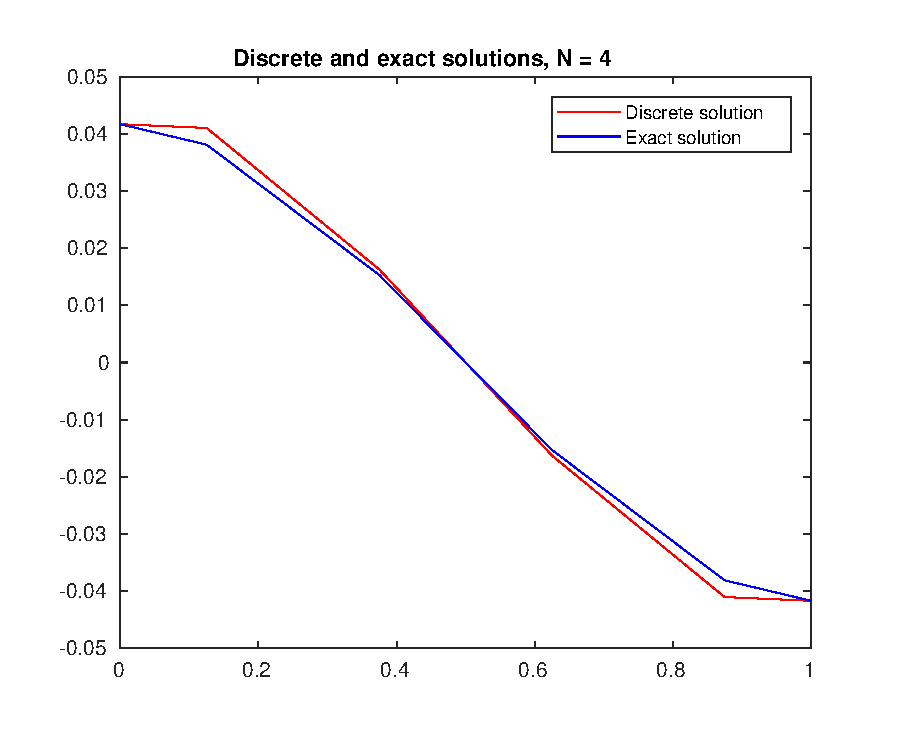
\includegraphics[width=10.5cm]{fig_dirichlet_result_uniform_midpoint_N4_C1}
\caption{Dirichlet result, uniform mesh, midpoint, Case 1, $N=4$.}
\end{figure}
\begin{figure}[H]
\centering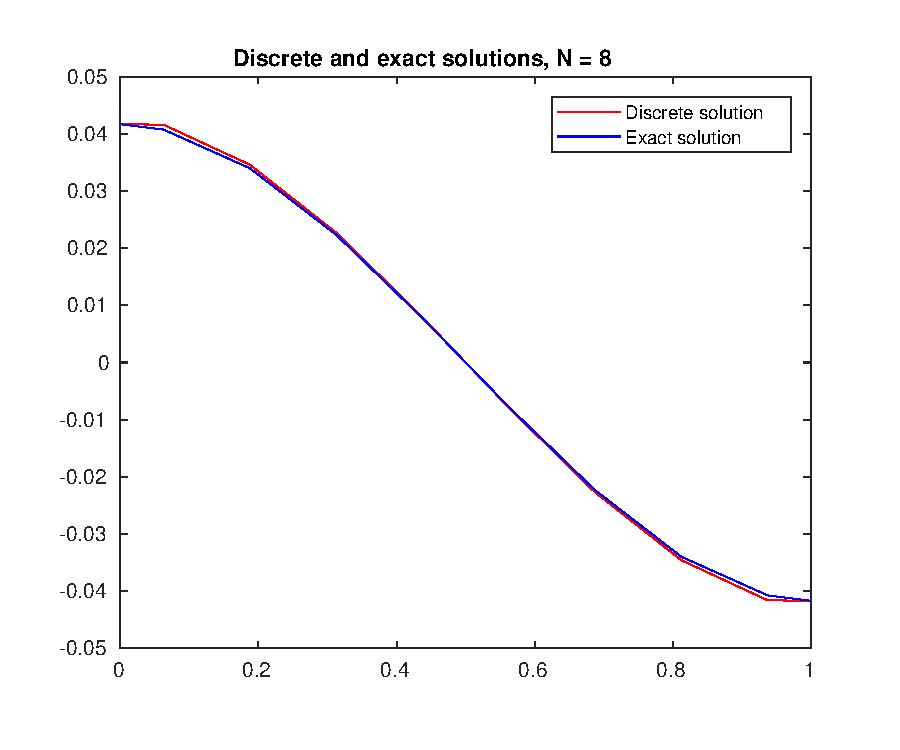
\includegraphics[width=10.5cm]{fig_dirichlet_result_uniform_midpoint_N8_C1}
\caption{Dirichlet result, uniform mesh, midpoint rule, Case 1, $N=8$.}
\end{figure}
\begin{figure}[H]
\centering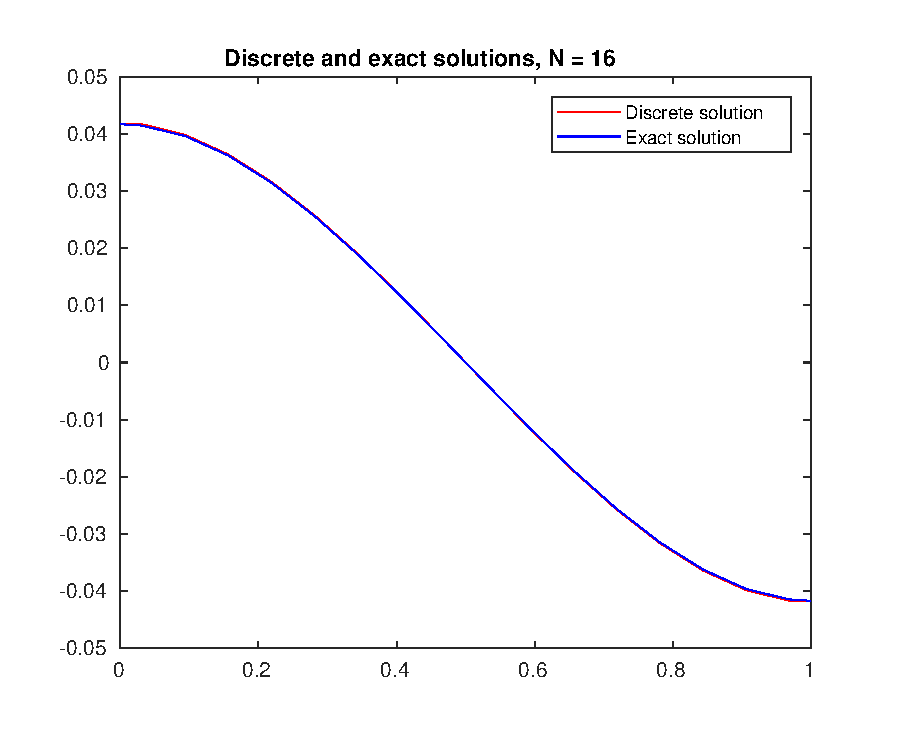
\includegraphics[width=10.5cm]{fig_dirichlet_result_uniform_midpoint_N16_C1}
\caption{Dirichlet result, uniform mesh, midpoint rule, Case 1, $N=16$.}
\end{figure}
\begin{figure}[H]
\centering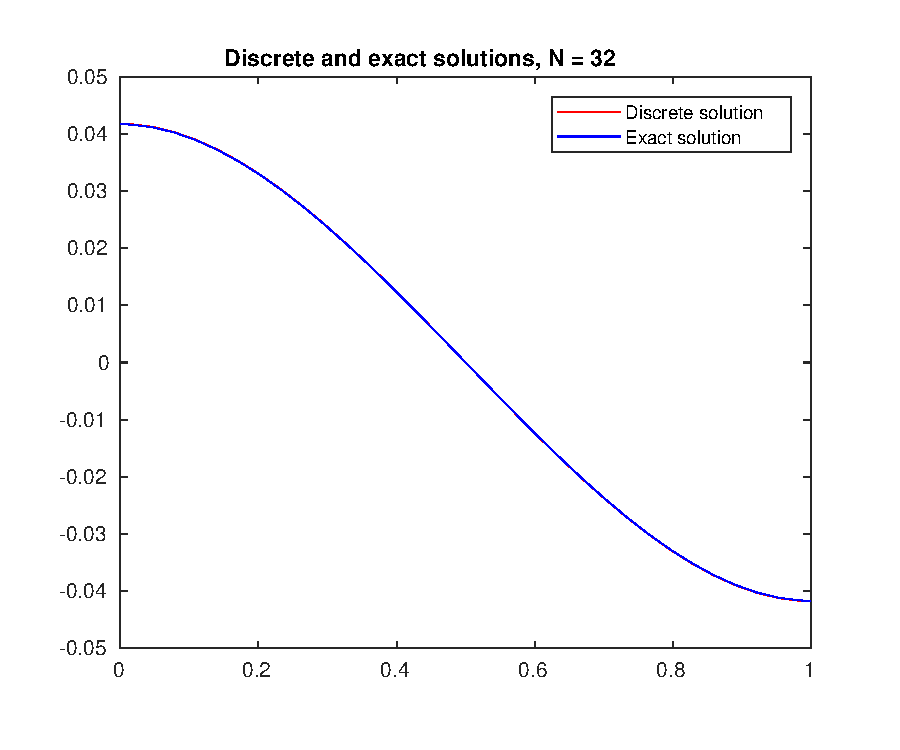
\includegraphics[width=10.5cm]{fig_dirichlet_result_uniform_midpoint_N32_C1}
\caption{Dirichlet result, uniform mesh, midpoint rule, Case 1, $N=32$.}
\end{figure}
\begin{figure}[H]
\centering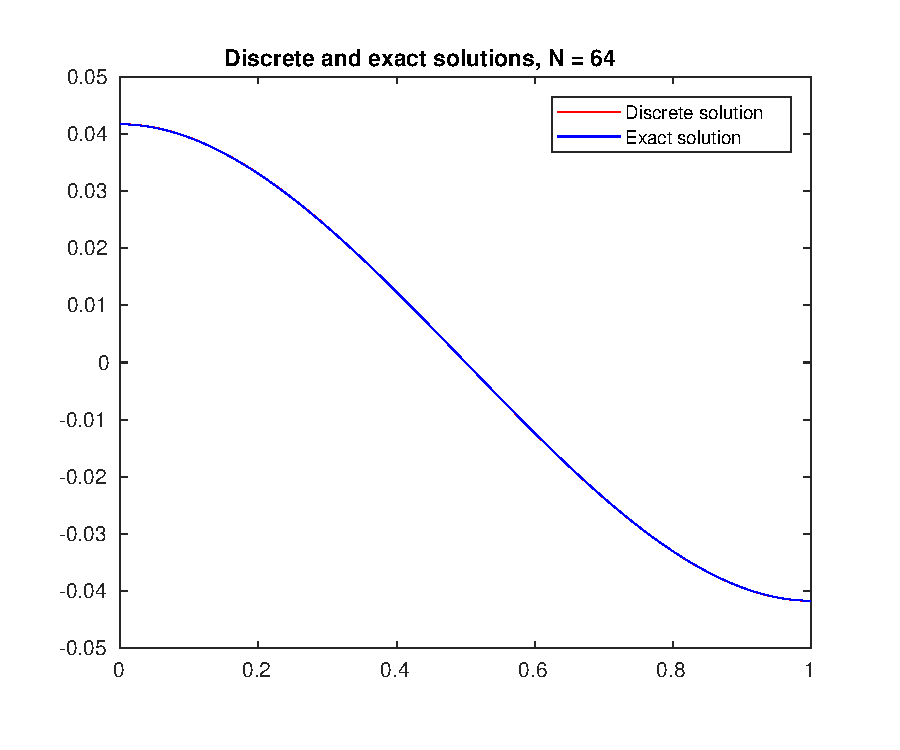
\includegraphics[width=10.5cm]{fig_dirichlet_result_uniform_midpoint_N64_C1}
\caption{Dirichlet result, uniform mesh, midpoint rule, Case 1, $N=64$.}
\end{figure}
\begin{figure}[H]
\centering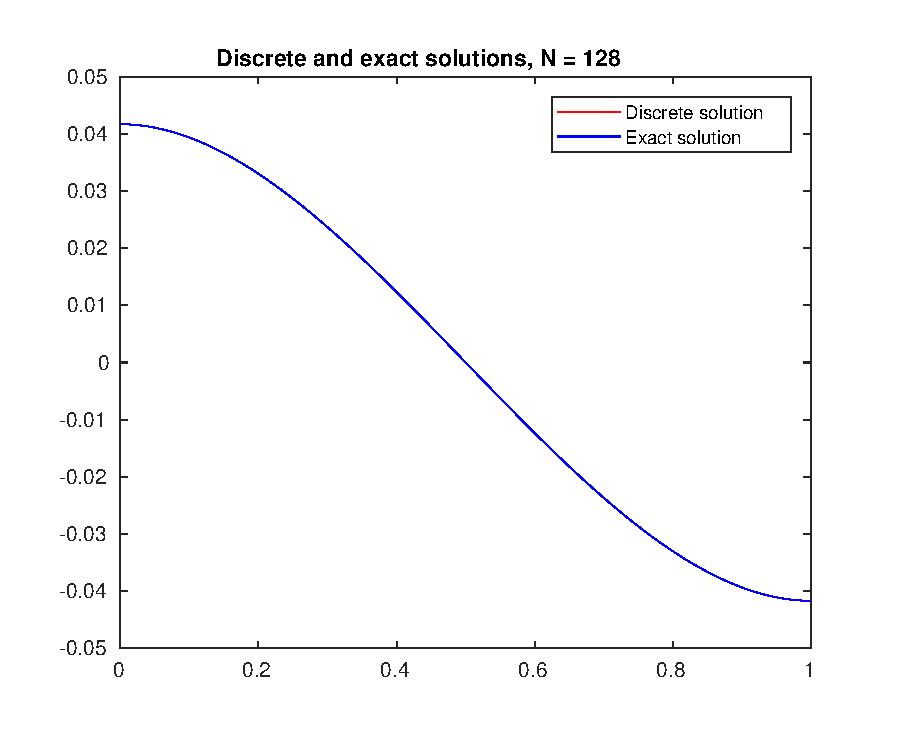
\includegraphics[width=10.5cm]{fig_dirichlet_result_uniform_midpoint_N128_C1}
\caption{Dirichlet result, uniform mesh, midpoint rule, Case 1, $N=128$.}
\end{figure}
\newpage
 \textsc{Case 2.}
\begin{figure}[H]
\centering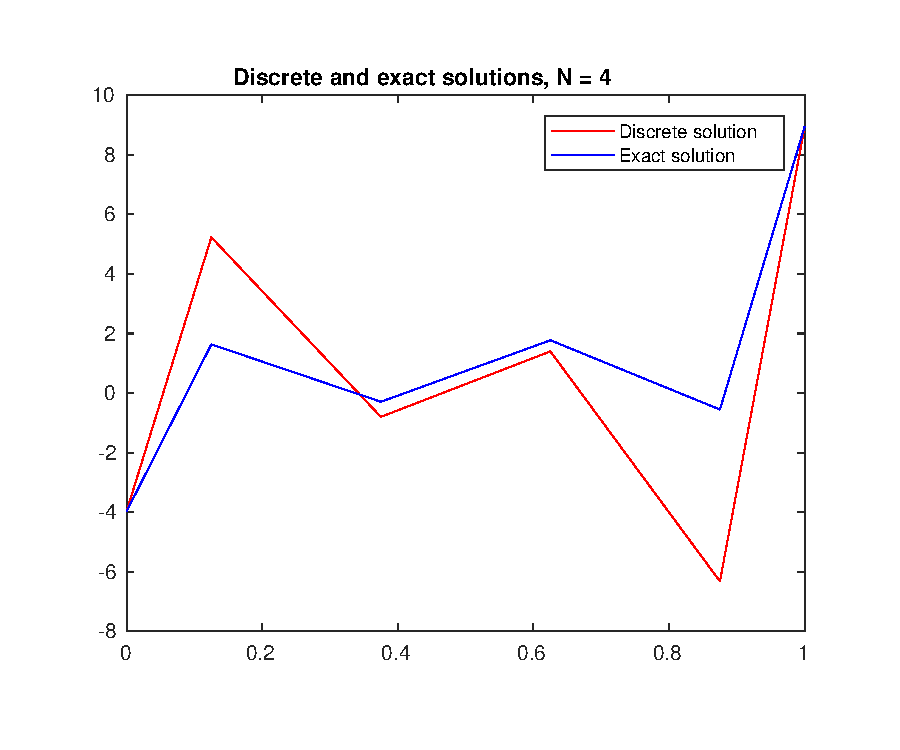
\includegraphics[width=10.5cm]{fig_dirichlet_result_uniform_midpoint_N4_C2}
\caption{Dirichlet result, uniform mesh, midpoint rule, Case 2, $N=4$.}
\end{figure}
\begin{figure}[H]
\centering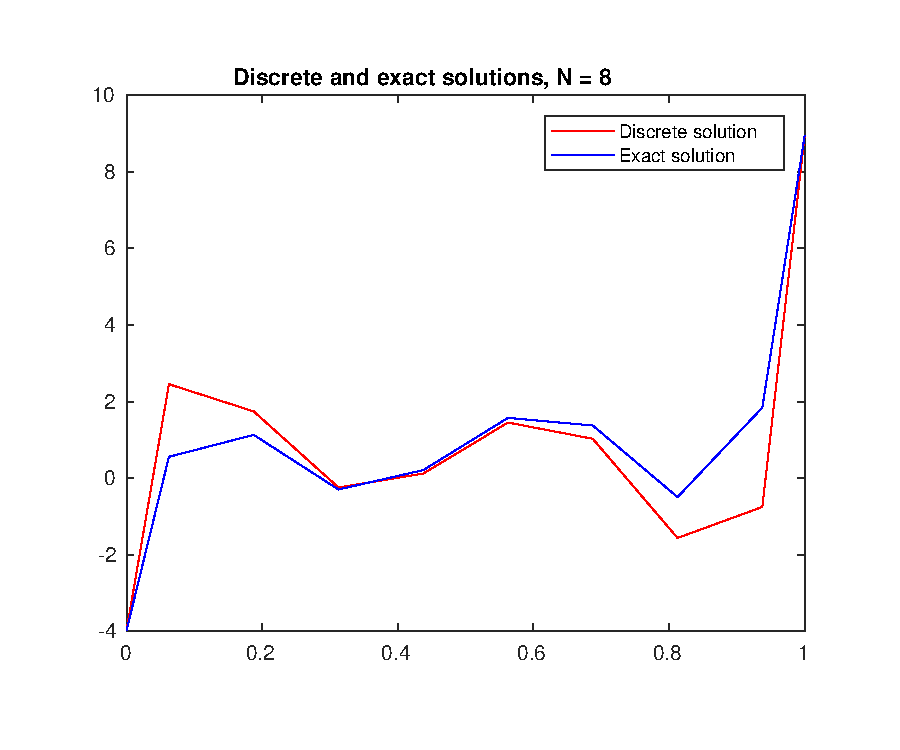
\includegraphics[width=10.5cm]{fig_dirichlet_result_uniform_midpoint_N8_C2}
\caption{Dirichlet result, uniform mesh, midpoint rule, Case 2, $N=8$.}
\end{figure}
\begin{figure}[H]
\centering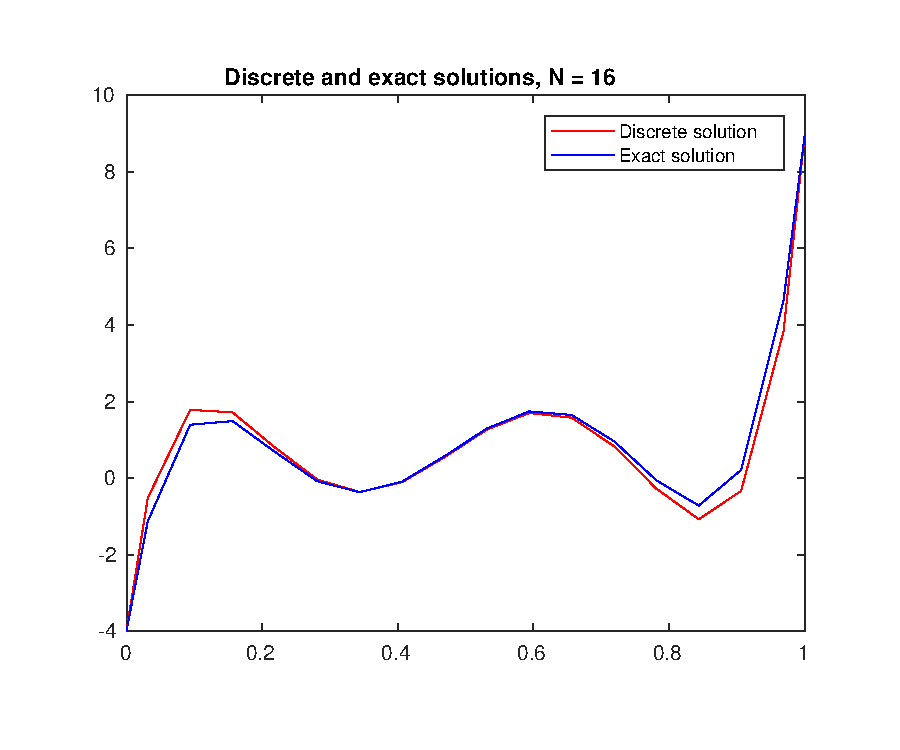
\includegraphics[width=10.5cm]{fig_dirichlet_result_uniform_midpoint_N16_C2}
\caption{Dirichlet result, uniform mesh, midpoint rule, Case 2, $N=16$.}
\end{figure}
\begin{figure}[H]
\centering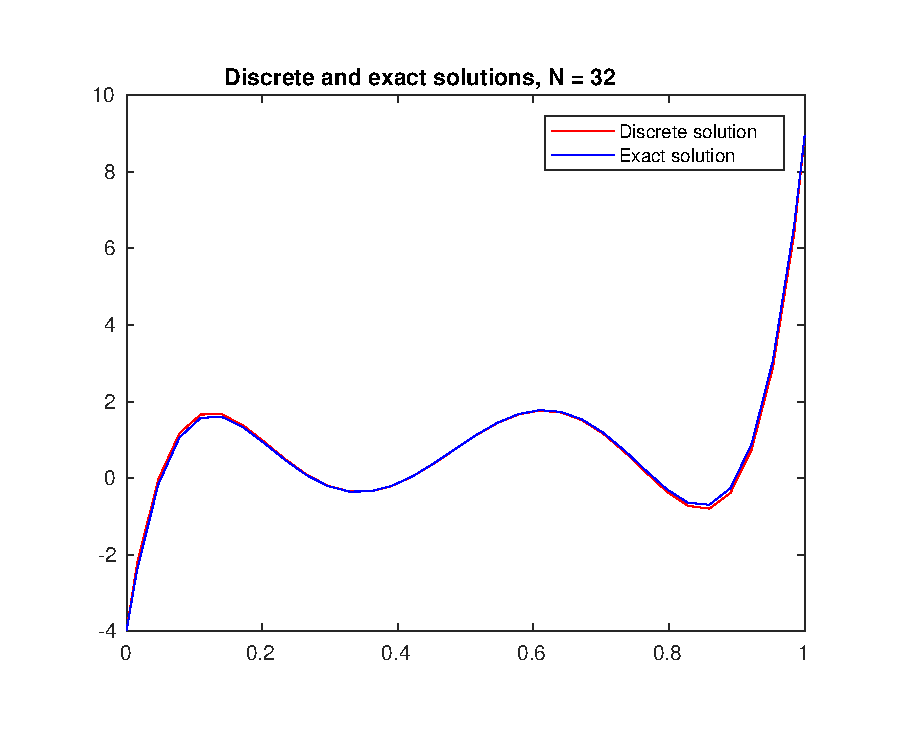
\includegraphics[width=10.5cm]{fig_dirichlet_result_uniform_midpoint_N32_C2}
\caption{Dirichlet result, uniform mesh, midpoint rule, Case 2, $N=32$.}
\end{figure}
\begin{figure}[H]
\centering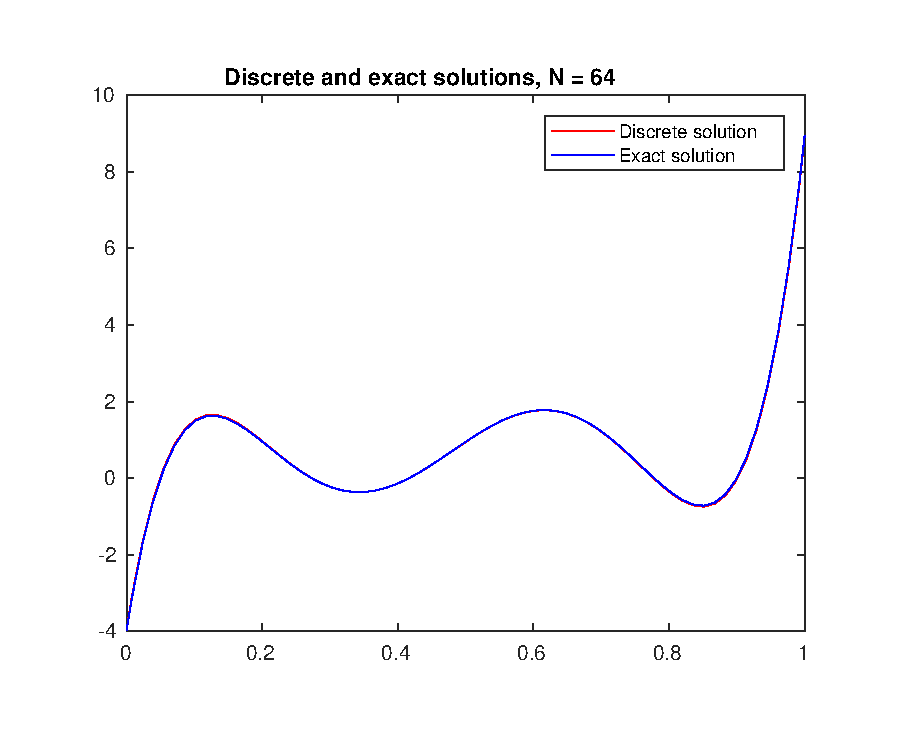
\includegraphics[width=10.5cm]{fig_dirichlet_result_uniform_midpoint_N64_C2}
\caption{Dirichlet result, uniform mesh, midpoint rule, Case 2, $N=64$.}
\end{figure}
\begin{figure}[H]
\centering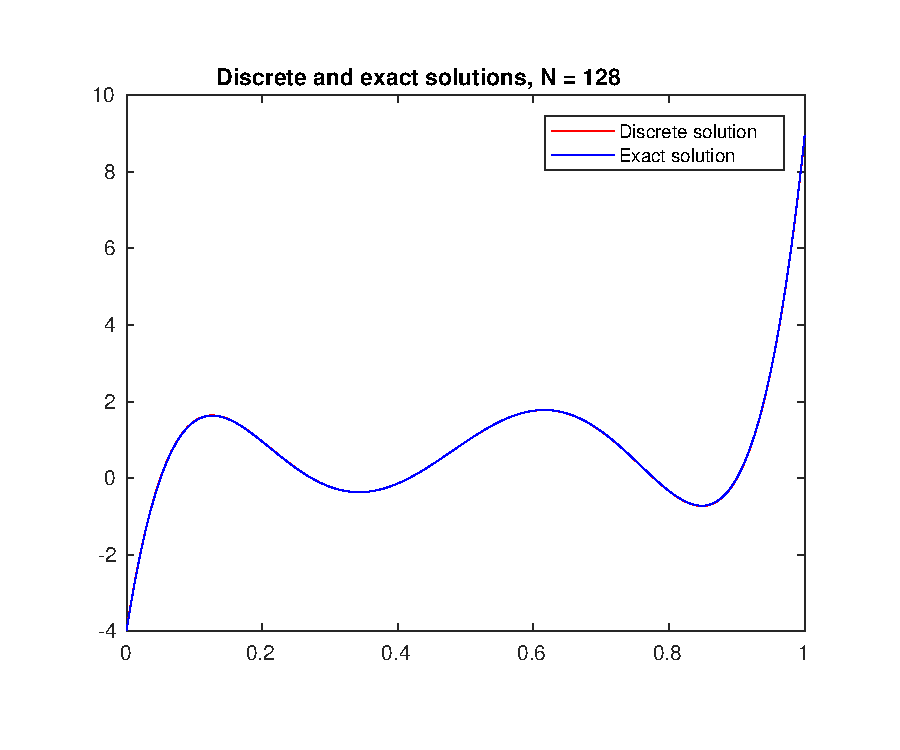
\includegraphics[width=10.5cm]{fig_dirichlet_result_uniform_midpoint_N128_C2}
\caption{Dirichlet result, uniform mesh, midpoint rule, Case 2, $N=128$.}
\end{figure}
\newpage
\textsc{Case 3.}
\begin{figure}[H]
\centering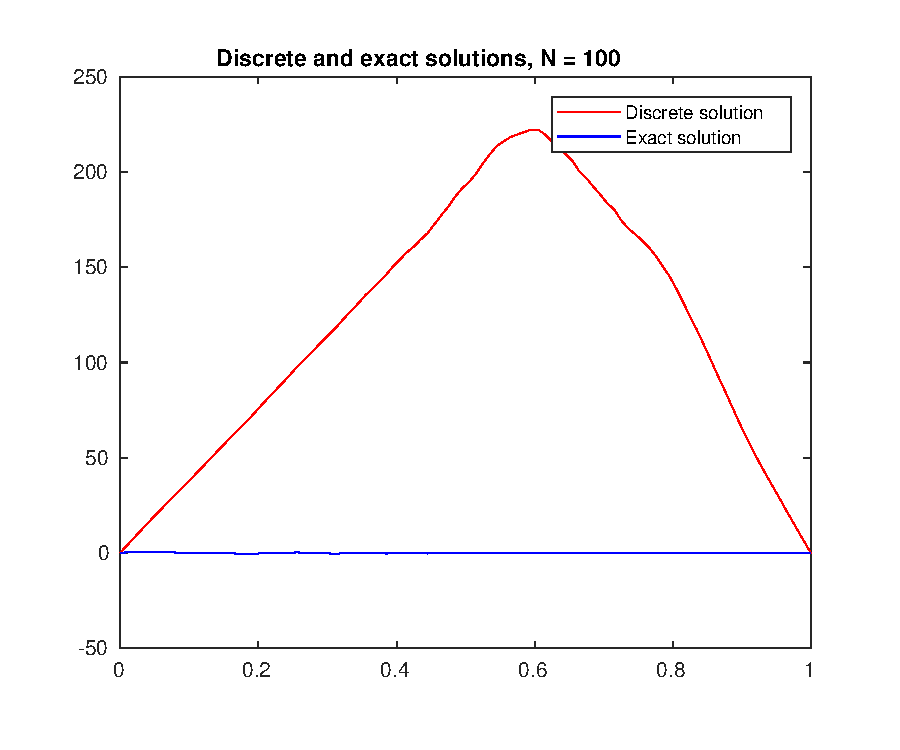
\includegraphics[width=10.5cm]{fig_dirichlet_result_uniform_midpoint_N100_C3}
\caption{Dirichlet result, uniform mesh, midpoint rule, Case 3, $N=100$.}
\end{figure}
\begin{figure}[H]
\centering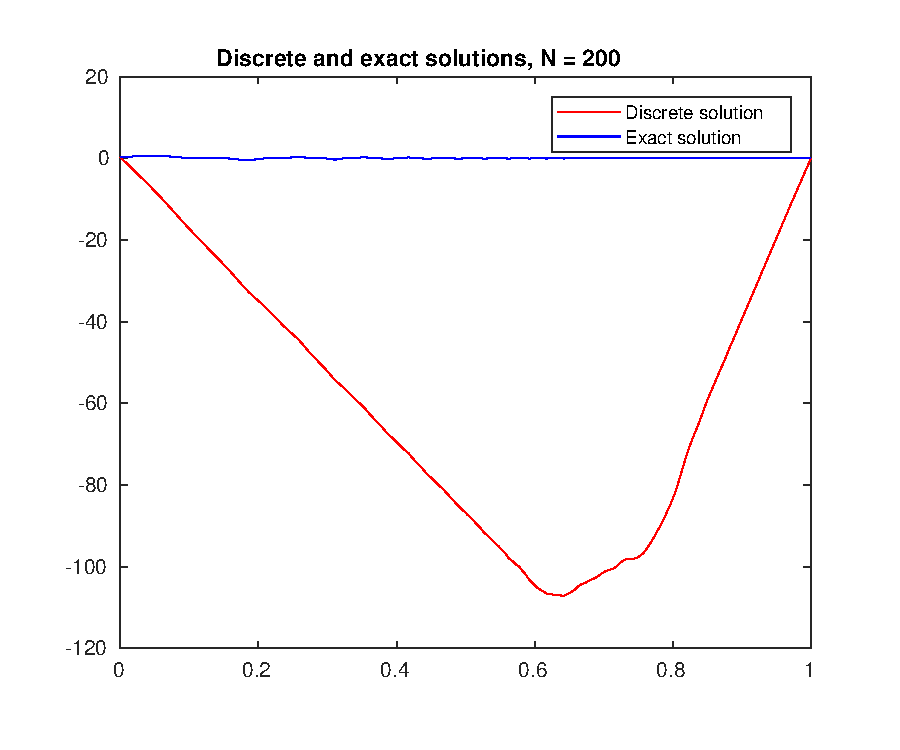
\includegraphics[width=10.5cm]{fig_dirichlet_result_uniform_midpoint_N200_C3}
\caption{Dirichlet result, uniform mesh, midpoint rule, Case 3, $N=200$.}
\end{figure}
\begin{figure}[H]
\centering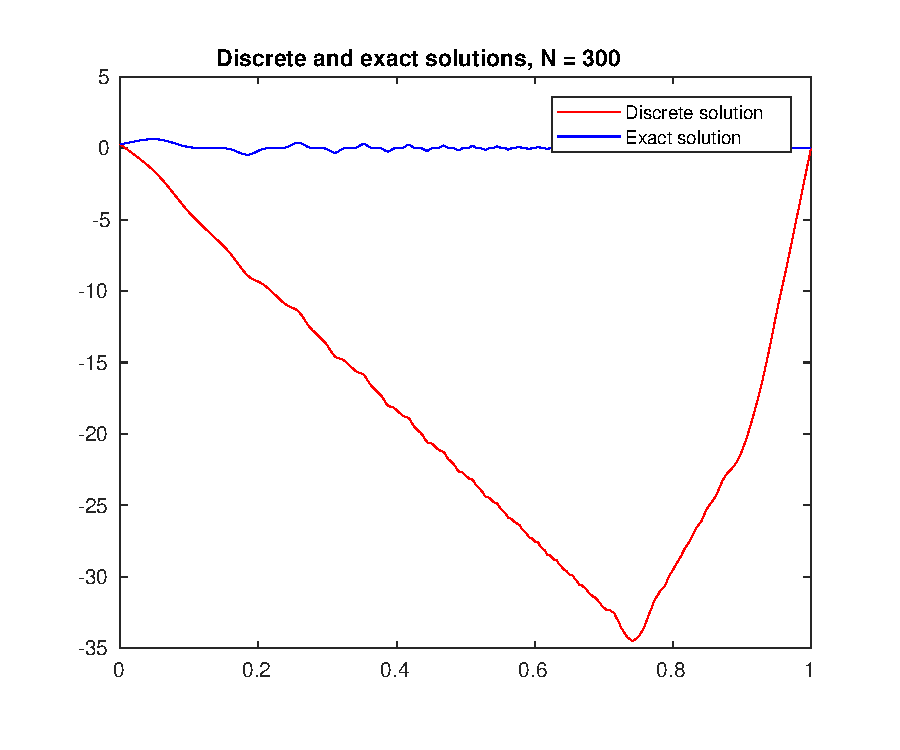
\includegraphics[width=10.5cm]{fig_dirichlet_result_uniform_midpoint_N300_C3}
\caption{Dirichlet result, uniform mesh, midpoint rule, Case 3, $N=300$.}
\end{figure}
\begin{figure}[H]
\centering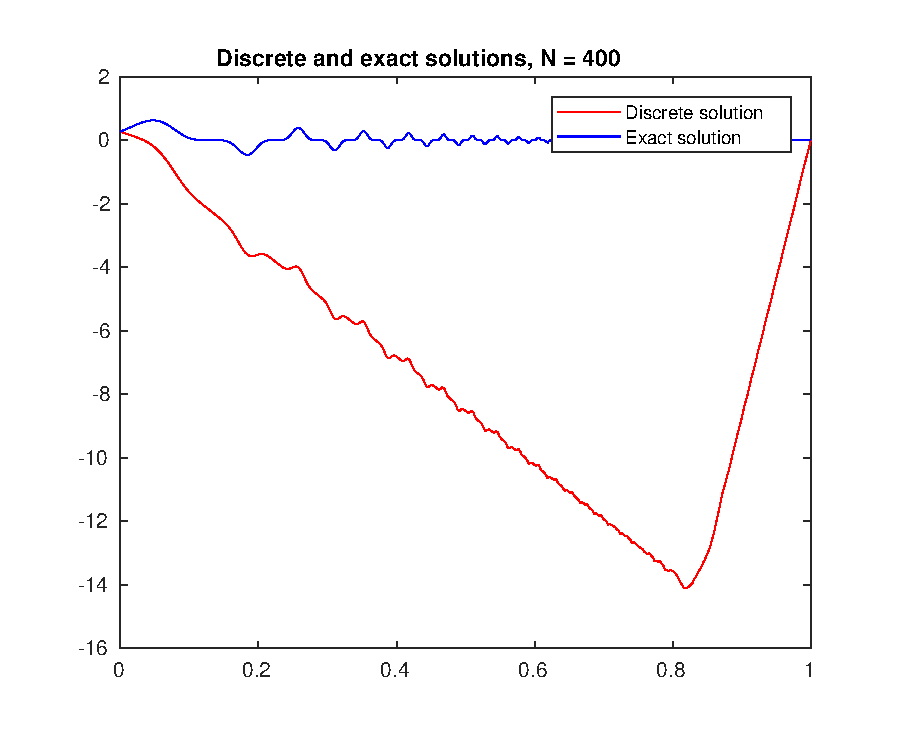
\includegraphics[width=10.5cm]{fig_dirichlet_result_uniform_midpoint_N400_C3}
\caption{Dirichlet result, uniform mesh, midpoint rule, Case 3, $N=400$.}
\end{figure}
\begin{figure}[H]
\centering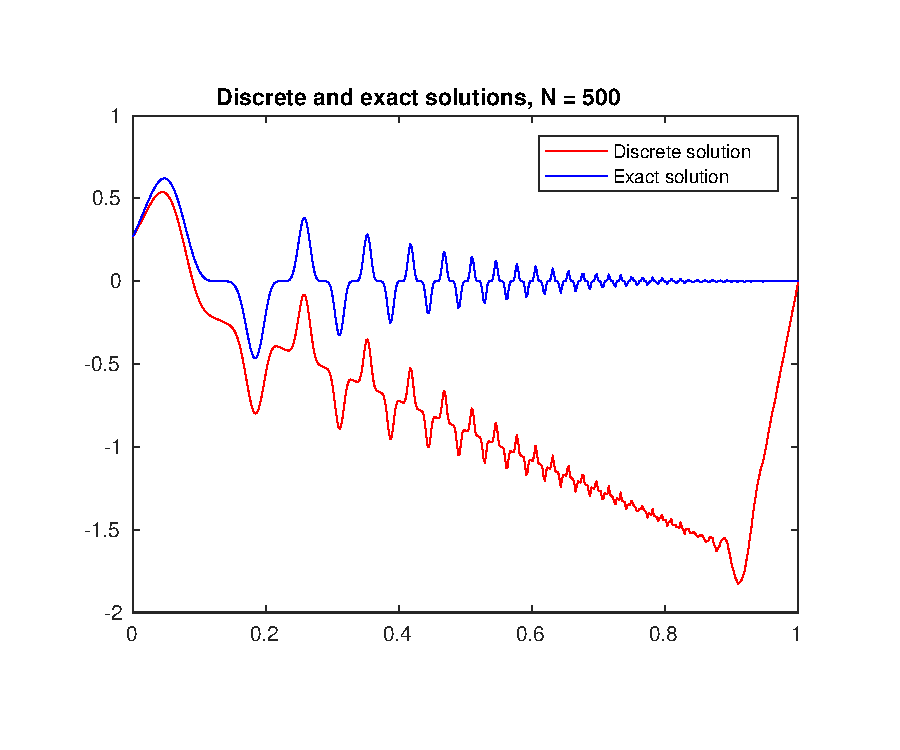
\includegraphics[width=10.5cm]{fig_dirichlet_result_uniform_midpoint_N500_C3}
\caption{Dirichlet result, uniform mesh, midpoint rule, Case 3, $N=500$.}
\end{figure}
\begin{figure}[H]
\centering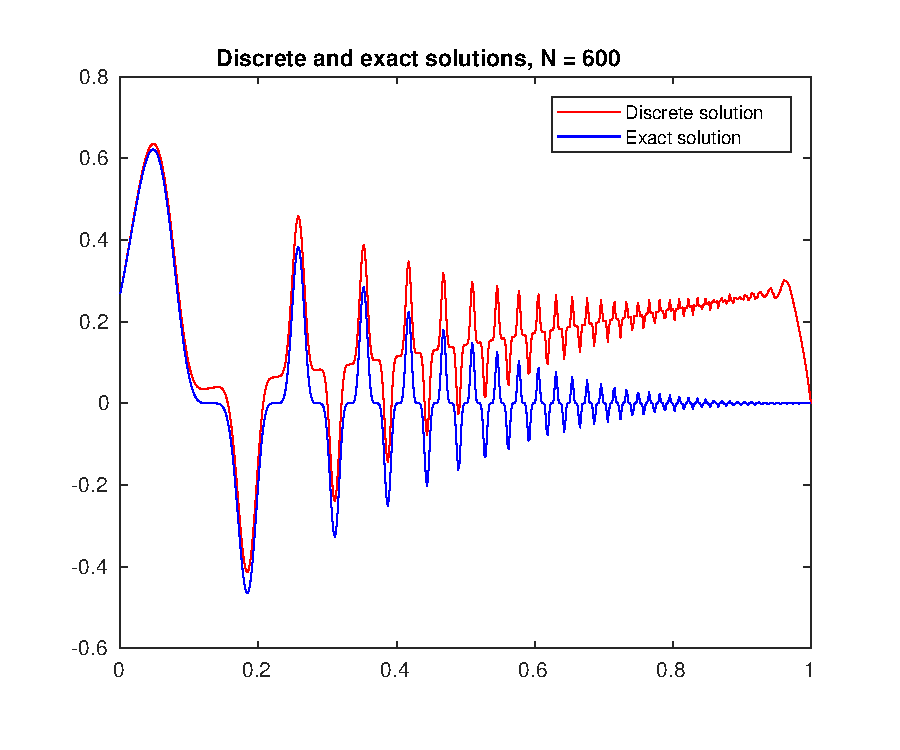
\includegraphics[width=10.5cm]{fig_dirichlet_result_uniform_midpoint_N600_C3}
\caption{Dirichlet result, uniform mesh, midpoint rule, Case 3, $N=600$.}
\end{figure}
\begin{figure}[H]
\centering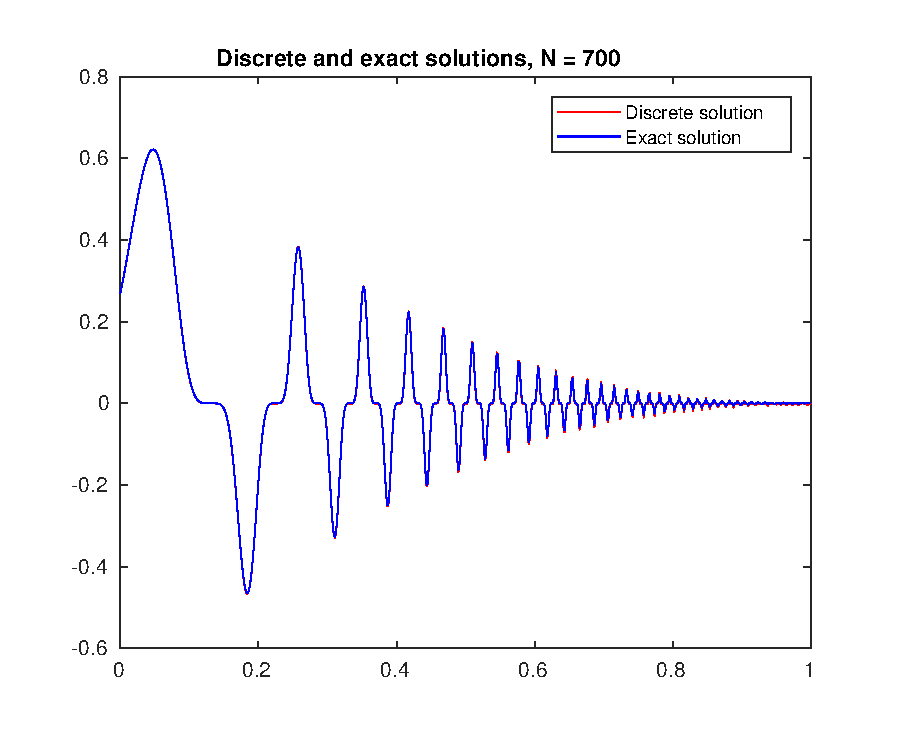
\includegraphics[width=10.5cm]{fig_dirichlet_result_uniform_midpoint_N700_C3}
\caption{Dirichlet result, uniform mesh, midpoint rule, Case 3, $N=700$.}
\end{figure}
\begin{figure}[H]
\centering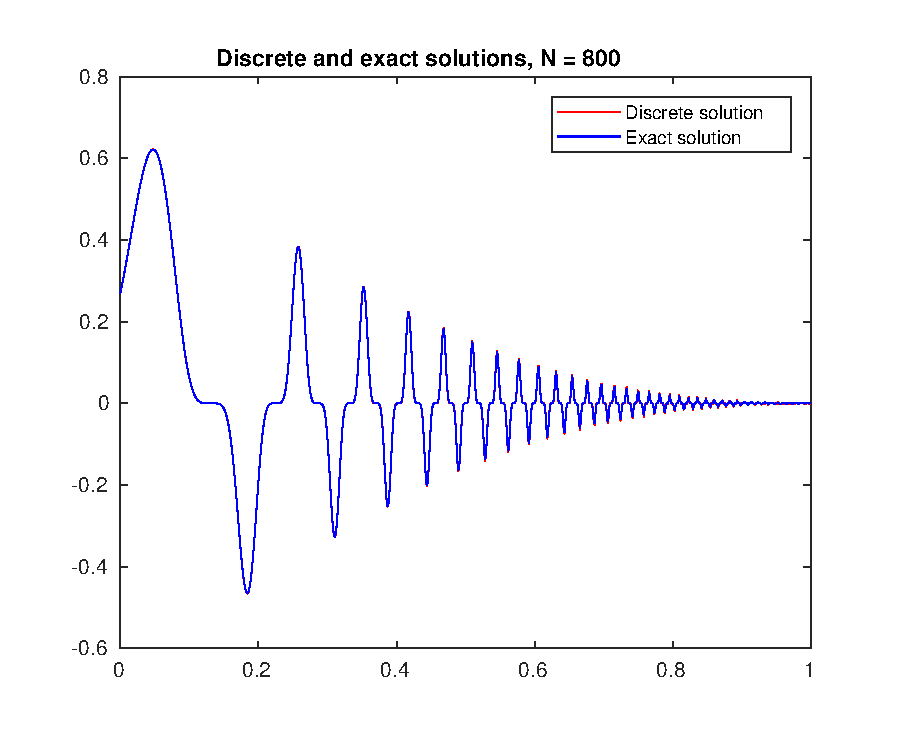
\includegraphics[width=10.5cm]{fig_dirichlet_result_uniform_midpoint_N800_C3}
\caption{Dirichlet result, uniform mesh, midpoint rule, Case 3, $N=800$.}
\end{figure}
\newpage
\subsubsection{Errors}
\textsc{Case 1.}
\begin{table}[H]
\centering
\begin{tabu}{|c|c|c|}
\hline
			$N$	&  $\lVert u_{discrete}-u_{exact}\rVert_{L^2}$& $\lVert u_{discrete}-u_{exact}\rVert_{H^1}$ \\\hline
			4	& 2.183660e-03 & 1.353165e-02 \\\hline
			8	& 5.593964e-04 & 5.167483e-03 \\\hline
			16	& 1.406791e-04 & 1.891105e-03 \\\hline
			32	& 3.522145e-05 & 6.796587e-04 \\\hline
			64	& 8.808591e-06 & 2.422258e-04 \\\hline
			128	& 2.202349e-06 & 8.597891e-05 \\\hline
\end{tabu}
\caption{Error table, Case 1.}
\end{table}
\noindent
\textsc{Case 2.}
\begin{table}[H]
\centering
\begin{tabu}{|c|c|c|}
\hline
			$N$	&  $\lVert u_{discrete}-u_{exact}\rVert_{L^2}$& $\lVert u_{discrete}-u_{exact}\rVert_{H^1}$ \\\hline
			4	& 3.414525e+00 & 1.723527e-02 \\\hline
			8	& 1.224066e+00 & 1.429127e+01 \\\hline
			16	& 3.297560e-01 & 6.028506e+00 \\\hline
			32	& 8.393195e-02 & 2.295482e+00 \\\hline
			64	& 2.107644e-02 & 8.397813e-01 \\\hline
			128	& 5.274953e-03 & 3.018207e-01 \\\hline
\end{tabu}
\caption{Error table, Case 2.}
\end{table}
\noindent
\textsc{Case 3.}
\begin{table}[H]
\centering
\begin{tabu}{|c|c|c|}
\hline
			$N$	&  $\lVert u_{discrete}-u_{exact}\rVert_{L^2}$& $\lVert u_{discrete}-u_{exact}\rVert_{H^1}$ \\\hline
			100	& 1.372029e+02 & 4.718806e+02 \\\hline
			200	& 6.795356e+01 & 2.432018e+02 \\\hline
			300	& 2.068556e+01 & 8.656798e+01 \\\hline
			400	& 8.220398e+00 & 3.814539e+01 \\\hline
			500	& 9.637916e-01 & 7.476626e+00 \\\hline
			600	& 1.613099e-01 & 2.708167e+00 \\\hline
			700	& 1.691419e-03 & 1.378369e+00 \\\hline
			800	& 1.035571e-03 & 1.034955e+00 \\\hline
\end{tabu}
\caption{Error table, Case 3.}
\end{table}

\newpage
\subsubsection{Convergence Rate}
\textsc{Case 1.}
\begin{figure}[H]
\centering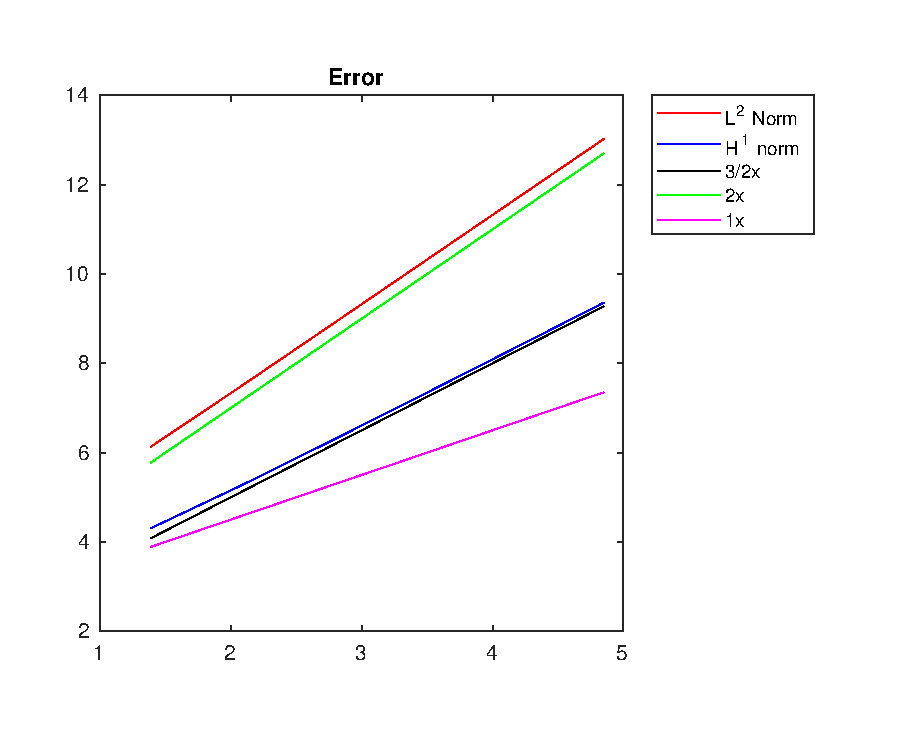
\includegraphics[width=13.5cm]{fig_dirichlet_error_midpoint_cp_uniform_midpoint_C1_M6}
\caption{Dirichlet error, midpoint rule, uniform mesh, Case 1.}
\end{figure}
\newpage
\noindent
\textsc{Case 2.}
\begin{figure}[H]
\centering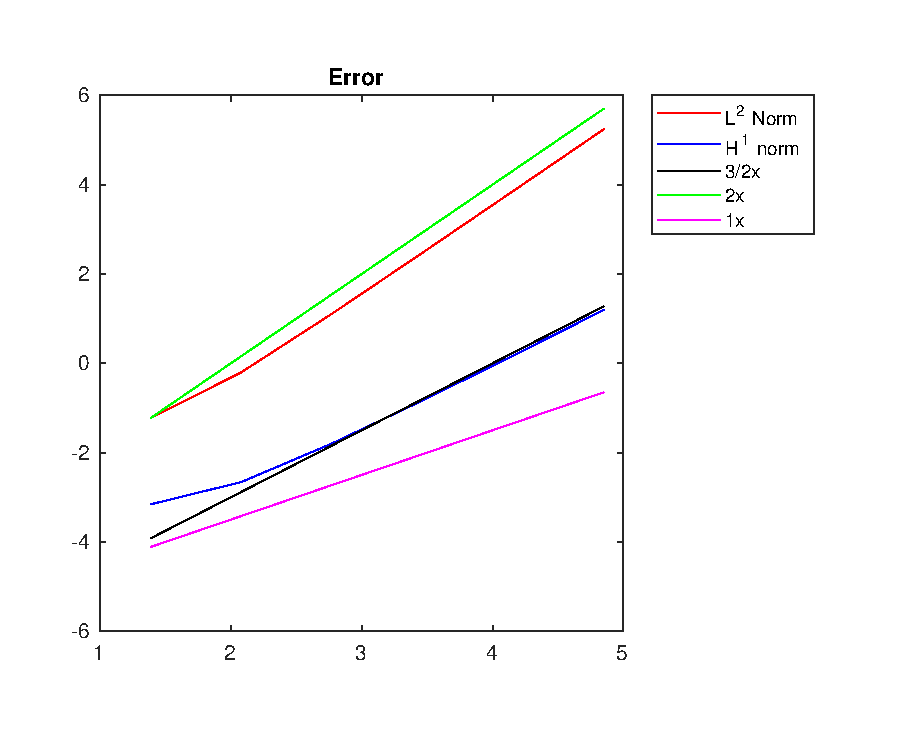
\includegraphics[width=13.5cm]{fig_dirichlet_error_midpoint_cp_uniform_midpoint_C2_M6}
\caption{Dirichlet error, midpoint rule, uniform mesh, Case 3.}
\end{figure}
\newpage
\noindent
\textsc{Case 3.}
\begin{figure}[H]
\centering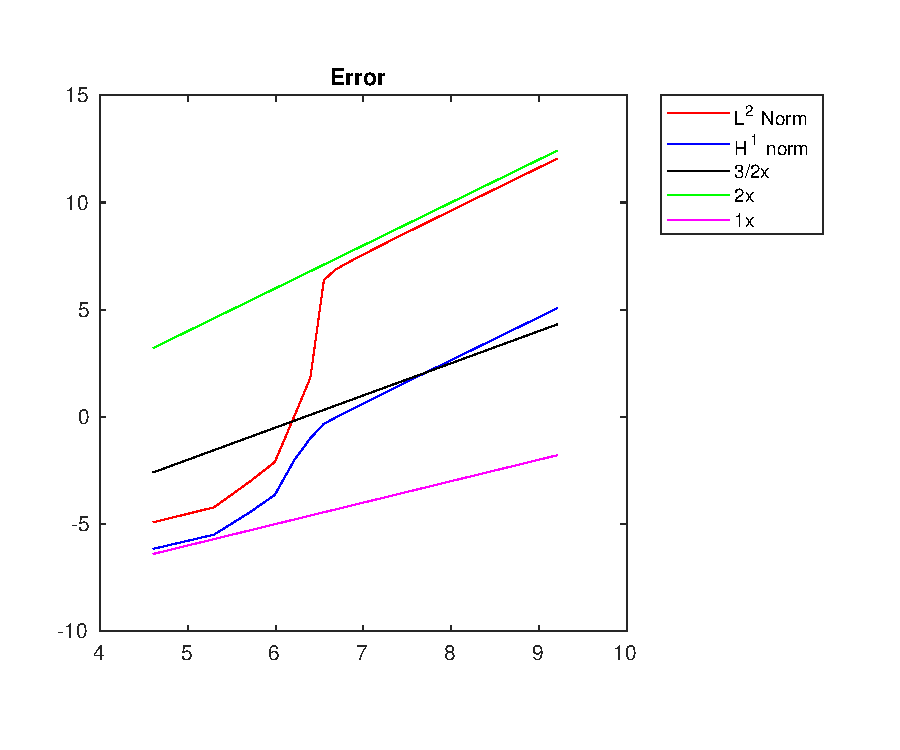
\includegraphics[width=13.5cm]{fig_dirichlet_error_midpoint_cp_uniform_midpoint_C3_M100}
\caption{Dirichlet error, midpoint rule, uniform mesh, Case 3.}
\end{figure}
\noindent\textbf{Remark 7.1.} We can see that in case 1 and case 2, the finite volume method has convergence rate of order $2$ in $L^2$ norm and order $\frac{3}{2}$ in energy norm. But in case 3, finite volume method has convergence rate of order $2$ in both $L^2$ and energy norm. Moreover, the convergence rate in case 3 only become consistent after the grid refinement reached a certain degree.
\newpage
\subsection{Homogeneous Dirichlet boundary condition, regular grid, each control point is $\frac{1}{3}$ from the left of corresponding control volume, integration using midpoint rule}
\subsubsection{Errors}
\textsc{Case 1.}
\begin{table}[H]
\centering
\begin{tabu}{|c|c|c|}
\hline
			$N$	&  $\lVert u_{discrete}-u_{exact}\rVert_{L^2}$& $\lVert u_{discrete}-u_{exact}\rVert_{H^1}$ \\\hline
			4	& 4.337732e-03 & 1.723527e-02 \\\hline
			8	& 1.976011e-03 & 7.696433e-03 \\\hline
			16	& 9.604458e-04 & 3.489791e-03 \\\hline
			32	& 4.766545e-04 & 1.633552e-03 \\\hline
			64	& 2.378772e-04 & 7.855739e-04 \\\hline
			128	& 1.188822e-04 & 3.845069e-04\\\hline
\end{tabu}
\caption{Error table, Case 1.}
\end{table}
\noindent
\textsc{Case 2.}
\begin{table}[H]
\centering
\begin{tabu}{|c|c|c|}
\hline
			$N$	&  $\lVert u_{discrete}-u_{exact}\rVert_{L^2}$& $\lVert u_{discrete}-u_{exact}\rVert_{H^1}$ \\\hline
			4	& 6.063755e+00 & 2.989757e+01 \\\hline
			8	& 3.072003e+00 & 1.824323e+01 \\\hline
			16	& 1.453481e+00 & 8.493182e+00\\\hline
			32	& 7.060401e-01 & 3.804418e+00\\\hline
			64	& 3.484227e-01 & 1.738566e+00 \\\hline
			128	& 1.731597e-01 & 8.193746e-01\\\hline
\end{tabu}
\caption{Error table, Case 2.}
\end{table}
\noindent
\textsc{Case 3.}
\begin{table}[H]
\centering
\begin{tabu}{|c|c|c|}
\hline
			$N$	&  $\lVert u_{discrete}-u_{exact}\rVert_{L^2}$& $\lVert u_{discrete}-u_{exact}\rVert_{H^1}$ \\\hline
			100	& 1.374387e+02 & 4.724692e+02 \\\hline
			200	& 6.805998e+01 & 2.434741e+02 \\\hline
			300	& 2.074894e+01 & 8.685629e+01 \\\hline
			400	& 8.237658e+00 & 3.826618e+01 \\\hline
			500	& 9.680948e-01 & 7.883261e+00 \\\hline
			600	& 1.628207e-01 & 3.371928e+00 \\\hline
			700	& 4.196379e-03 & 2.193966e+00 \\\hline
			800	& 3.381889e-03 & 1.786729e+00 \\\hline
\end{tabu}
\caption{Error table, Case 3.}
\end{table}
\newpage
\subsubsection{Convergence rate}
\noindent\textsc{Case 1.}
\begin{figure}[H]
\centering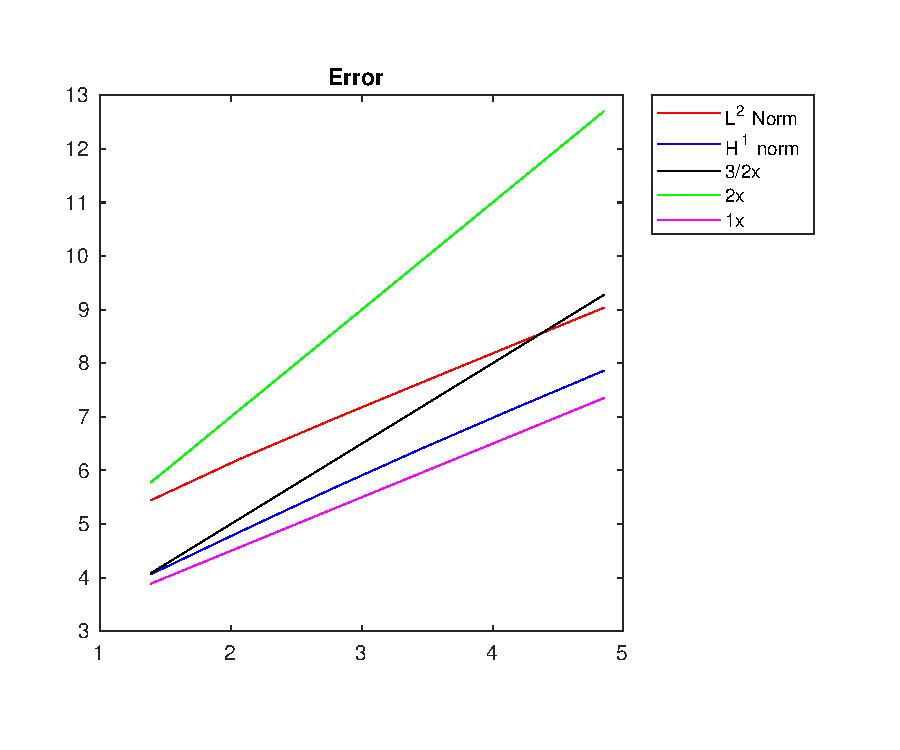
\includegraphics[width=13.5cm]{fig_dirichlet_error_left_cp_uniform_midpoint_C1_M6}
\caption{Dirichlet error left, uniform mesh, midpoint rule, Case 1.}
\end{figure}
\newpage
\noindent
\textsc{Case 2.}
\begin{figure}[H]
\centering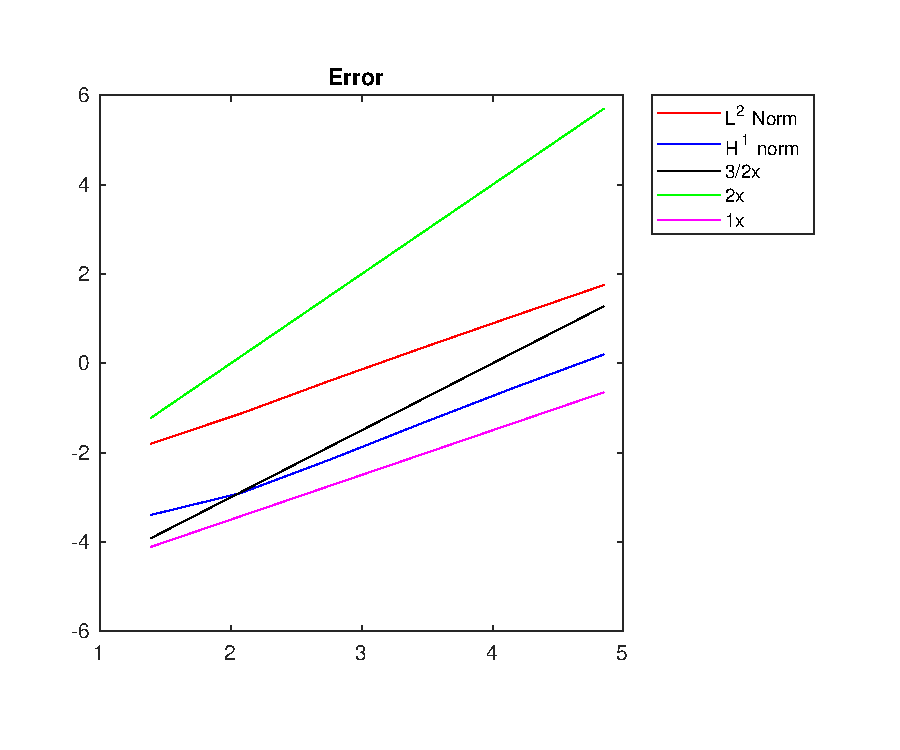
\includegraphics[width=13.5cm]{fig_dirichlet_error_left_cp_uniform_midpoint_C2_M6}
\caption{Dirichlet error left, uniform mesh, midpoint rule, Case 2.}
\end{figure}
\newpage
\noindent
\textsc{Case 3.}
\begin{figure}[H]
\centering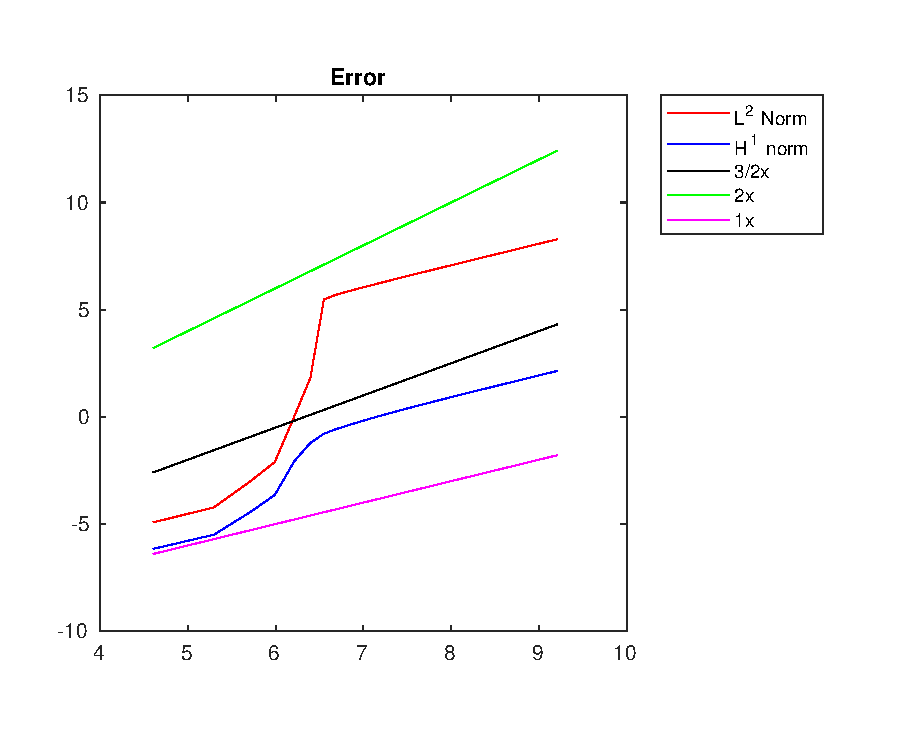
\includegraphics[width=13.5cm]{fig_dirichlet_error_left_cp_uniform_midpoint_C3_M100}
\caption{Dirichlet error left, uniform mesh, midpoint rule, Case 3.}
\end{figure}
\noindent\textbf{Remark 7.2.} Unlike the results in previous section, in all 3 cases, the finite volume method has convergence rate of order $1$ in both $L^p$ and energy norm. However, in case 3, similar to before, the convergence rate in case 3 only become consistent after the grid refinement reached a certain degree.
\subsection{Approximation of the Mean Value of the Function $f$ Over Control Volumes}
\subsubsection{Some Integral Approximation Rules}
	There are many ways to approximate integrals, both with equally spaced integration points and unequally spaced integration points. However, we are going to test only a few way of approximation with equally spaced integration points.

We need to approximate 
\begin{align}
\frac{1}{x_{i+\frac{1}{2}}-x_{i-\frac{1}{2}}}\int_{x_{i-\frac{1}{2}}}^{x_{i+\frac{1}{2}}}f(x)
\end{align}
with $T_i=\left[x_{i-\frac{1}{2}},x_{i+\frac{1}{2}}\right]$ being the control volume on which we need to approximate the mean value of $f$. For the sake of convenience, let $a=x_{i-\frac{1}{2}}$ and $b=x_{i+\frac{1}{2}}$.\\
\\
\textbf{Midpoint rule\index{midpoint rule}.}
\begin{align}
\frac{1}{b-a}\int_{a}^{b}f(x)&=\frac{1}{b-a}(b-a)f\left(\frac{a+b}{2}\right)-\frac{1}{b-a}\frac{(b-a)^3}{24}f^{(2)}(\xi)\\
		&=f\left(\frac{a+b}{2}\right)-\frac{(b-a)^2}{24}f^{(2)}(\xi)
\end{align}
For some $\xi$ in $[a,b]$.\hfill $\square$\\
\\
\textbf{Trapezoidal rule\index{trapezoidal rule}.}
\begin{align}
\frac{1}{b-a}\int_{a}^{b}f(x)&=\frac{1}{b-a}\frac{b-a}{2}(f(a)+f(b))-\frac{1}{b-a}\frac{1}{12}(b-a)^3f^{(2)}(\xi)\\
	&=\frac{f(a)+f(b)}{2}-\frac{1}{12}(b-a)^2f^{(2)}(\xi)
\end{align}
For some $\xi$ in $[a,b]$.\hfill $\square$\\
\\
\textbf{Simpson's rule\index{Simpson's rule}.} Let $h=\frac{b-a}{2}$, $t_1=a$, $t_2=a+h=\frac{b-a}{2}$, $t_3=a+2h=b$.
\begin{align}
\frac{1}{b-a}\int_{a}^{b}f(x)&=\frac{1}{2h}\frac{1}{3}\left(f(t_1)+4f(t_2)+f(t_3)\right)+\frac{1}{2h}\frac{1}{90}h^5f^{(4)}(\xi)\\
	&=\frac{1}{6h}\left(f(t_1)+4f(t_2)+f(t_3)\right)+\frac{1}{180}h^4f^{(4)}(\xi)
\end{align}
For some $\xi$ in $[a,b]$.\hfill $\square$\\
\\
\textbf{Boole's rule\index{Boole's rule}.} Let $h=\frac{b-a}{4}$, $t_1=a$, $t_2=a+h$, $t_3=a+2h$, $t_4=a+3h$, $t_5=a+4h=b$.
\begin{align}
&\frac{1}{b-a}\int_{a}^{b}f(x)\\
&=\frac{h}{90}\left(7f(t_1)+32f(t_2)+12f(t_3)+32f(t_4)+7f(t_5)\right)-\frac{8h^7}{945}f^{(6)}(\xi)&
\end{align}
For some $\xi$ in $[a,b]$.\hfill $\square$\\
\subsubsection{Effects in the Finite Volume Method}
In this section, we will test case 3 with various integral approximation rules.
\newpage
\noindent
\textbf{Errors.}
\begin{table}[H]
\centering
\begin{tabu}{|c|c|c|}
\hline
			$N$	&  $\lVert u_{discrete}-u_{exact}\rVert_{L^2}$& $\lVert u_{discrete}-u_{exact}\rVert_{H^1}$ \\\hline
			100	& 1.372029e+02 & 4.718806e+02 \\\hline
			200	& 6.795356e+01 & 2.432018e+02 \\\hline
			300	& 2.068556e+01 & 8.656798e+01 \\\hline
			400	& 8.220398e+00 & 3.814539e+01 \\\hline
			500	& 9.637916e-01 & 7.476626e+00 \\\hline
			600	& 1.613099e-01 & 2.708167e+00 \\\hline
			700	& 1.691419e-03 & 1.378369e+00 \\\hline
			800	& 1.035571e-03 & 1.034955e+00 \\\hline
\end{tabu}
\caption{Error table - Midpoint rule.}
\end{table}
\begin{table}[H]
\centering
\begin{tabu}{|c|c|c|}
\hline
			$N$	&  $\lVert u_{discrete}-u_{exact}\rVert_{L^2}$& $\lVert u_{discrete}-u_{exact}\rVert_{H^1}$ \\\hline
			100	& 3.773644e+01 & 2.412211e+02 \\\hline
			200	& 8.391778e+01 & 3.030967e+02 \\\hline
			300	& 2.038450e+01 & 8.486880e+01 \\\hline
			400	& 8.220498e+00 & 3.799774e+01 \\\hline
			500	& 9.637879e-01 & 7.212178e+00 \\\hline
			600	& 1.612986e-01 & 2.251598e+00 \\\hline
			700	& 1.234248e-03 & 8.617033e-01 \\\hline
			800	& 5.799255e-04 & 6.097104e-01 \\\hline
\end{tabu}
\caption{Error table - Trepozoidal rule.}
\end{table}

\begin{table}[H]
\centering
\begin{tabu}{|c|c|c|}
\hline
			$N$	&  $\lVert u_{discrete}-u_{exact}\rVert_{L^2}$& $\lVert u_{discrete}-u_{exact}\rVert_{H^1}$ \\\hline
			100	& 1.014161e+02 & 3.530643e+02 \\\hline
			200	& 1.742818e+01 & 6.491145e+01 \\\hline
			300	& 6.995754e+00 & 2.947754e+01 \\\hline
			400	& 2.740099e+00 & 1.278054e+01 \\\hline
			500	& 3.212656e-01 & 2.611736e+00 \\\hline
			600	& 5.377526e-02 & 1.087361e+00 \\\hline
			700	& 7.420314e-04 & 6.371791e-01 \\\hline
			800	& 4.998059e-04 & 4.889503e-01 \\\hline
\end{tabu}
\caption{Error table - Simpson's rule.}
\end{table}
\begin{table}[H]
\centering
\begin{tabu}{|c|c|c|}
\hline
			$N$	&  $\lVert u_{discrete}-u_{exact}\rVert_{L^2}$& $\lVert u_{discrete}-u_{exact}\rVert_{H^1}$ \\\hline
			100	& 2.543855e+01 & 9.312152e+01 \\\hline
			200	& 1.936562e+00 & 1.267931e+01 \\\hline
			300	& 5.423098e-01 & 3.614971e+00 \\\hline
			400	& 1.670127e-01 & 1.894852e+00 \\\hline
			500	& 3.154194e-02 & 1.063986e+00 \\\hline
			600	& 1.971232e-03 & 8.160713e-01 \\\hline
			700	& 6.508166e-04 & 5.954282e-01 \\\hline
			800	& 4.865046e-04 & 4.672134e-01 \\\hline
\end{tabu}
\caption{Error table - Boole's rule.}
\end{table}
\noindent\textbf{Remark 7.3.} We can see that there are some variation in the accuracy when using different integration methods.\\
\\
\textbf{Convergence Rate.}\\
\textsc{Case 3, $M=100$.}
\begin{figure}[H]
\centering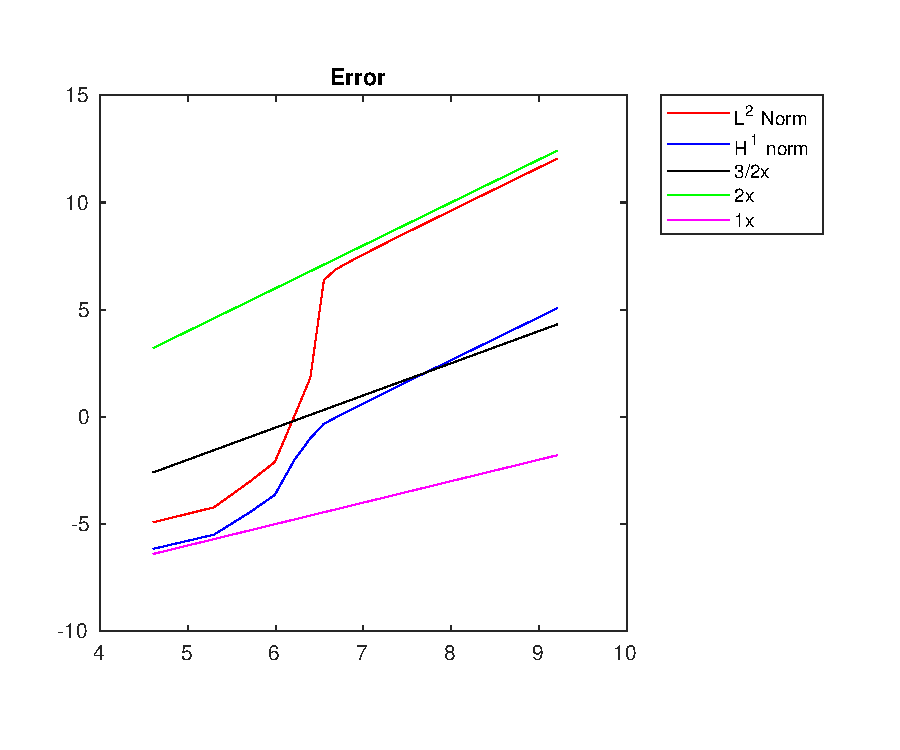
\includegraphics[width=13.5cm]{fig_dirichlet_error_midpoint_cp_uniform_midpoint_C3_M100}
\caption{Dirichlet error left, uniform mesh, midpoint rule, Case 3.}
\end{figure}
\newpage
\begin{figure}[H]
\centering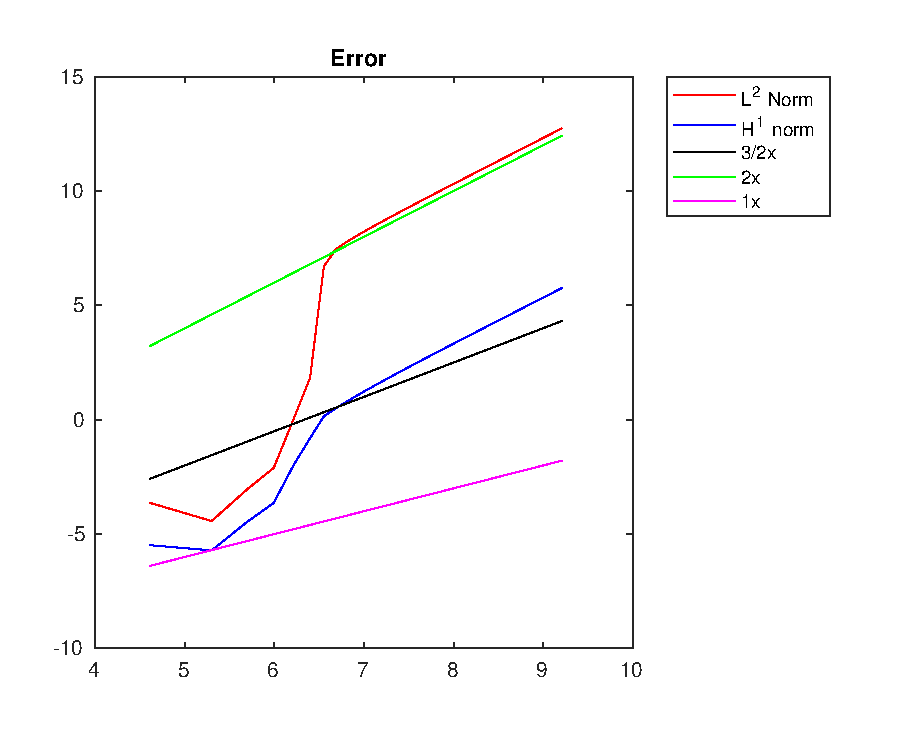
\includegraphics[width=13.5cm]{fig_dirichlet_error_midpoint_cp_uniform_trepozoidal_C3_M100}
\caption{Dirichlet error left, uniform mesh, trapezoidal rule, Case 3.}
\end{figure}
\newpage
\begin{figure}[H]
\centering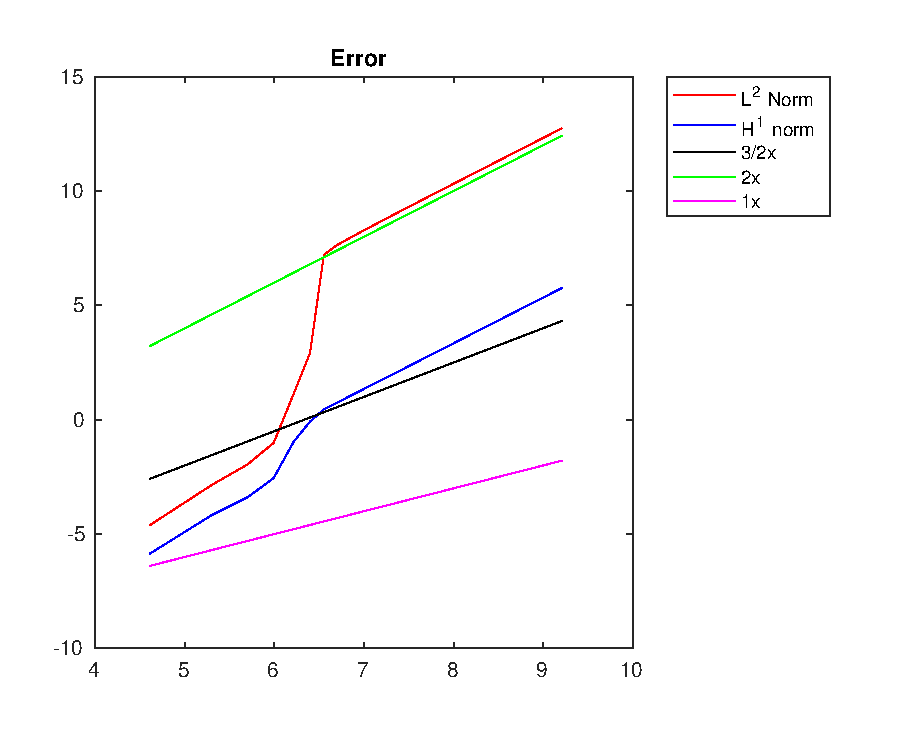
\includegraphics[width=13.5cm]{fig_dirichlet_error_midpoint_cp_uniform_simpson_C3_M100}
\caption{Dirichlet error left, uniform mesh, Simpson rule, Case 3.}
\end{figure}
\newpage
\begin{figure}[H]
\centering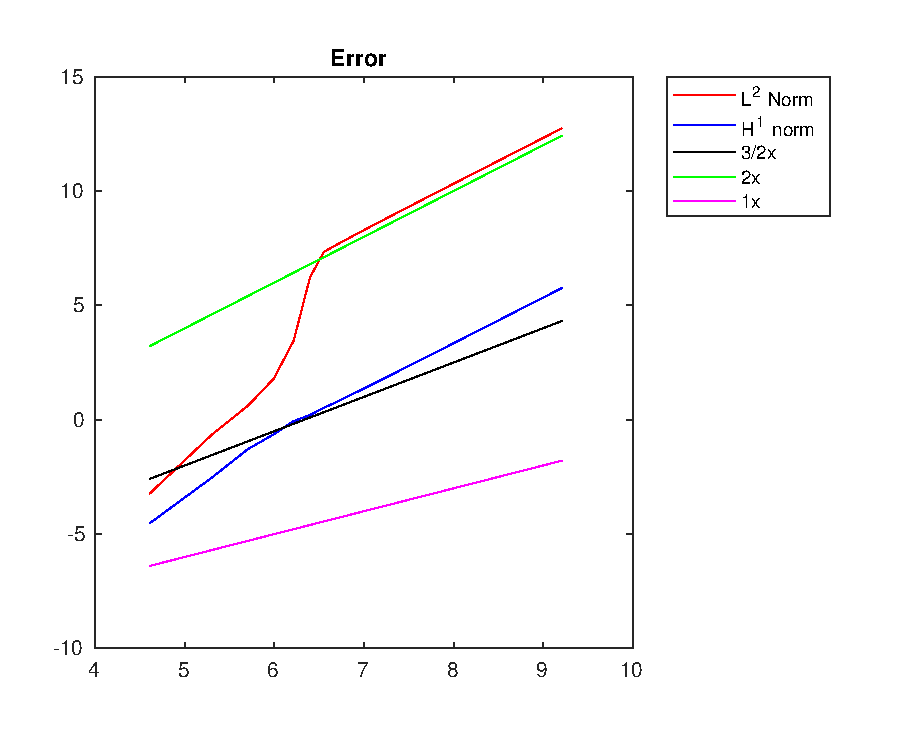
\includegraphics[width=13.5cm]{fig_dirichlet_error_midpoint_cp_uniform_boole_C3_M100}
\caption{Dirichlet error left, uniform mesh, Boole rule, Case 3.}
\end{figure}
\subsection{Homogeneous Dirichlet boundary condition, singular grid, each control point is the midpoint of corresponding control volume}
	In this section, we will consider the grid
\begin{align}
x_i=1-\cos\left(\frac{\pi i}{2(N+1)}\right)
\end{align}
\newpage
\subsubsection{Errors}
\textsc{Case 1.}
\begin{table}[H]
\centering
\begin{tabu}{|c|c|c|}
\hline
			$N$	&  $\lVert u_{discrete}-u_{exact}\rVert_{L^2}$& $\lVert u_{discrete}-u_{exact}\rVert_{H^1}$ \\\hline
			4	& 2.572594e-03 & 1.408303e-02 \\\hline
			8	& 8.312800e-04 & 6.052092e-03 \\\hline
			16	& 2.366590e-04 & 2.399498e-03 \\\hline
			32	& 6.309364e-05 & 9.021918e-04 \\\hline
			64	& 1.628265e-05 & 3.291959e-04 \\\hline
			128	& 4.135350e-06 & 1.182551e-04 \\\hline
\end{tabu}
\caption{Error table, Case 1.}
\end{table}
\noindent
\textsc{Case 2.}
\begin{table}[H]
\centering
\begin{tabu}{|c|c|c|}
\hline
			$N$	&  $\lVert u_{discrete}-u_{exact}\rVert_{L^2}$& $\lVert u_{discrete}-u_{exact}\rVert_{H^1}$ \\\hline
			4	& 5.147535e+00 & 2.212485e+01 \\\hline
			8	& 2.426569e+00 & 1.848306e+01 \\\hline
			16	& 7.617805e-01 & 9.789540e+00 \\\hline
			32	& 2.084740e-01 & 4.495505e+00 \\\hline
			64	& 5.417277e-02 & 2.011451e+00 \\\hline
			128	& 1.378284e-02 & 9.183423e-01 \\\hline
\end{tabu}
\caption{Error table, Case 2.}
\end{table}
\noindent
\textsc{Case 3.}
\begin{table}[H]
\centering
\begin{tabu}{|c|c|c|}
\hline
			$N$	&  $\lVert u_{discrete}-u_{exact}\rVert_{L^2}$& $\lVert u_{discrete}-u_{exact}\rVert_{H^1}$ \\\hline
			100	& 2.382533e+02 & 7.816445e+02 \\\hline
			200	& 1.021832e+02 & 3.524253e+02 \\\hline
			300	& 6.461806e+01 & 2.324792e+02 \\\hline
			400	& 3.011621e+01 & 1.225957e+02 \\\hline
			500	& 2.319667e+01 & 9.540720e+01 \\\hline
			600	& 1.878345e+00 & 1.109190e+01 \\\hline
			700	& 2.656605e+00 & 1.539149e+01 \\\hline
			800	& 2.128635e+00 & 1.401007e+01 \\\hline
			900	& 2.328867e-01 & 3.282076e+00\\\hline
			1000	& 1.798795e-02 & 1.705853e+00 \\\hline
			1100	& 1.554054e-03 & 1.344722e+00 \\\hline
			1200	& 1.011087e-03 & 1.052726e+00 \\\hline
\end{tabu}
\caption{Error table, Case 3.}
\end{table}
\newpage
\subsubsection{Convergence rate}
\textsc{Case 1.}
\begin{figure}[H]
\centering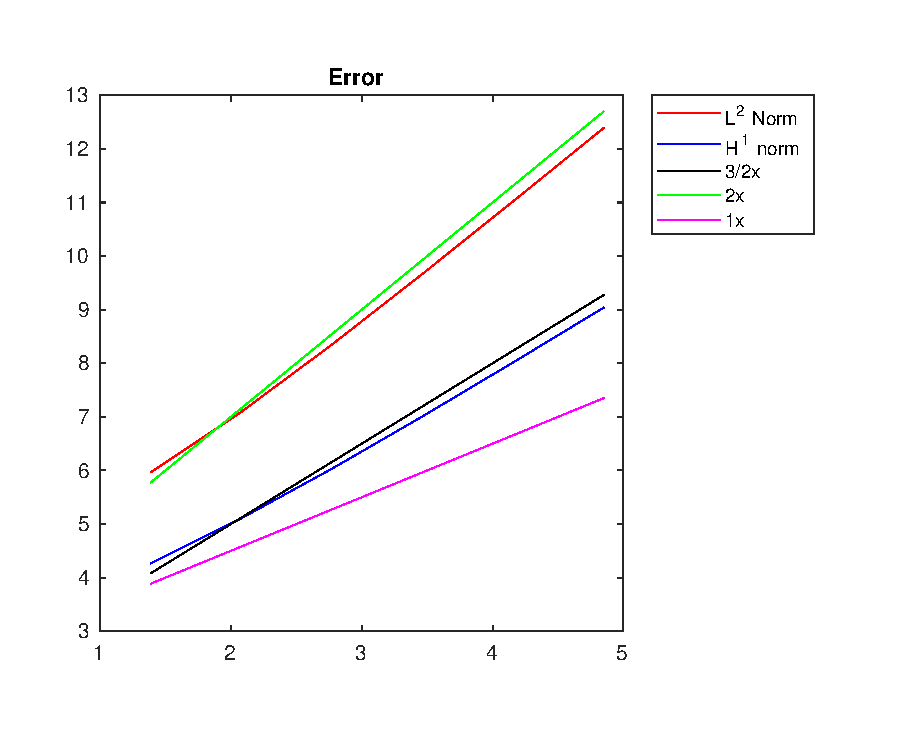
\includegraphics[width=13.5cm]{fig_dirichlet_error_G2_CP1_I1_M6_C1}
\caption{Dirichlet error, Case 1.}
\end{figure}
\newpage
\textsc{Case 2.}
\begin{figure}[H]
\centering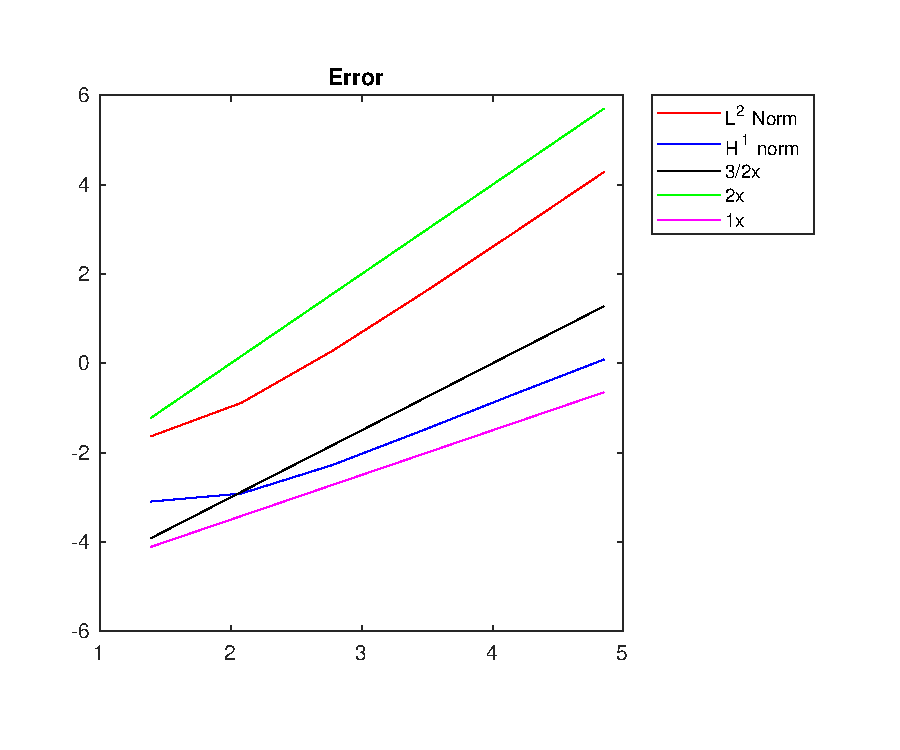
\includegraphics[width=13.5cm]{fig_dirichlet_error_G2_CP1_I1_M6_C2}
\caption{Dirichlet error, Case 2.}
\end{figure}
\newpage
\textsc{Case 3.}
\begin{figure}[H]
\centering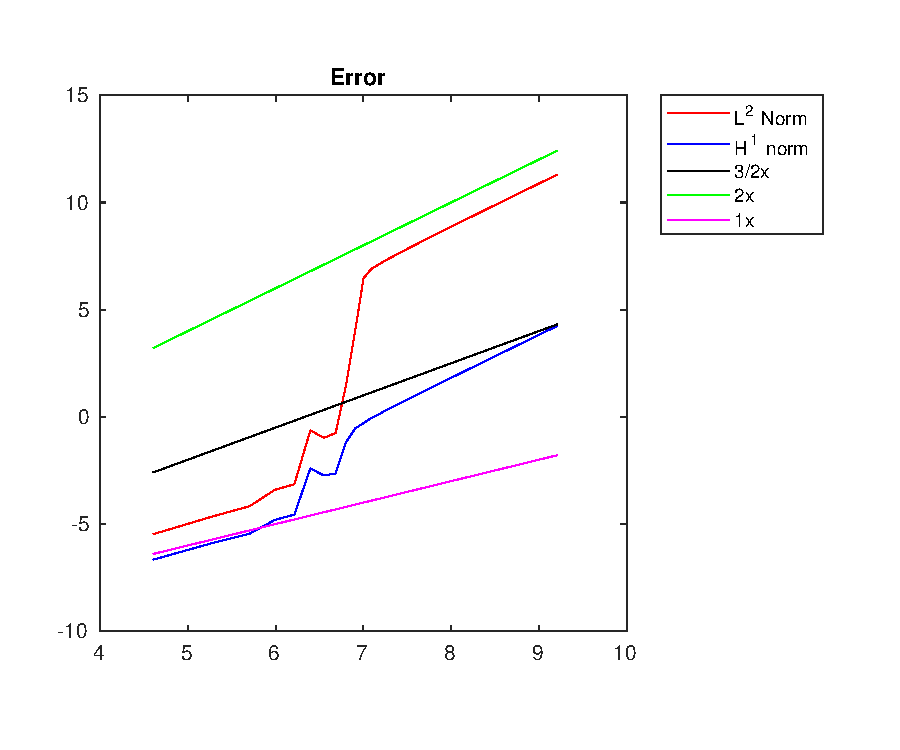
\includegraphics[width=13.5cm]{fig_dirichlet_error_G2_CP1_I1_M100_C3}
\caption{Dirichlet error, Case 3.}
\end{figure}
\noindent\textbf{Remark 7.4.}
\begin{enumerate}
\item In case 1, the method appears to have convergence rate of order $2$ in $L^2$ norm and order $\frac{3}{2}$ in energy norm.
\item In case 2, the method appears to have convergence rate of order $2$ in $L^2$ norm and order $1$ in energy norm.
\item In case 3, the method appears to have convergence rate of order $2$ in both $L^2$ energy norm and there are some ``irregularities'' in the convergence rate before the grid refinement reach a certain degree.
\end{enumerate}
\newpage
\section{Neumann boundary condition}
	In this section, we are going to test the Finite Volume Method for the one-dimensional Poisson equation subjected to Neumann boundary condition with several test cases using uniform grid and singular grid.
\subsection{Main Idea}
	We now review the problem we need to solve
\begin{align}
	-u''(x)&=f(x), \mbox{ in }\Omega \\
	u'(0)&=0 \\
	u'(1)&=0 \\
\int_{0}^{1}f(x)dx&=0 \\
\int_{0}^{1}u(x)dx&=0 \label{intu0}
\end{align}

	We note that if we omit the condition \eqref{intu0}, this problem will have infinitely many solutions of the form $u_1(x)+c$, with $u_1(x)$ being a solution of the problem.\\
	Let $U=\left[U_0, U_1, U_2, \dots,U_N, U_{N+1}\right]^t$ be the discrete solution of the problem.
	
When using derivative approximation with first order convergence rate, the boundary condition can be discretized as $U_0=U_1$ and $U_N=U_{N+1}$. Then, we need to use the linear system to solve for $U=\left[U_1, U_2, \dots,U_N\right]^t$.

We also note that the discretized linear system has one independent variable. Therefore, we can choose to solve for one solution $\overline{U}$ such that $U_k=0$ for some $k$ and then use the condition $\int_{0}^{1}u(x)dx=0$ to find the constant $C$ such that $U=\overline{U}+C$ satisfies the condition.\\

\subsection{Test cases}
\textsc{Case 1.}
\begin{align}
u(x)&=\frac{x^2\left(2x-3\right)}{12}+\frac{1}{24}\\
	f(x)&=\frac{1}{2}-x\\
\int_{0}^{1}f(x)&=0\\
	u'(0)&=0\\
	u'(1)&=0\\
	\int_{0}^{1}u(x)&=0
\end{align}
\noindent
\textsc{Case 2.}
\begin{align}
u(x)&=\sin\left(20\pi x +\frac{\pi}{2}\right)\\
	f(x)&=400\pi^2\cos\left(20\pi x\right)\\
\int_{0}^{1}f(x)&=0\\
	u'(0)&=0\\
	u'(1)&=0\\
	\int_{0}^{1}u(x)&=0
\end{align}
\subsection{Homogeneous Neumann boundary condition, regular grid, each control point is the midpoint of corresponding control volume, integration using midpoint rule}
\subsubsection{Figures of results}
\textsc{Case 1.}
\begin{figure}[H]
\centering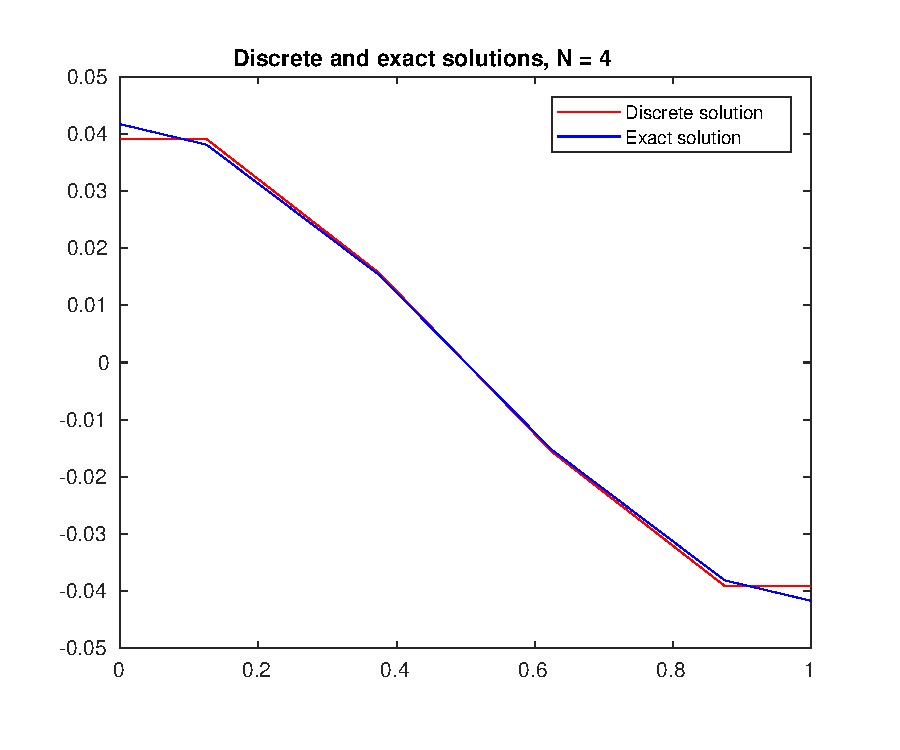
\includegraphics[width=10.5cm]{fig_neumann_result_G1_CP1_I1_N4_M6_C1}
\caption{Neumann result, $N=4$, Case 1.}
\end{figure}
\begin{figure}[H]
\centering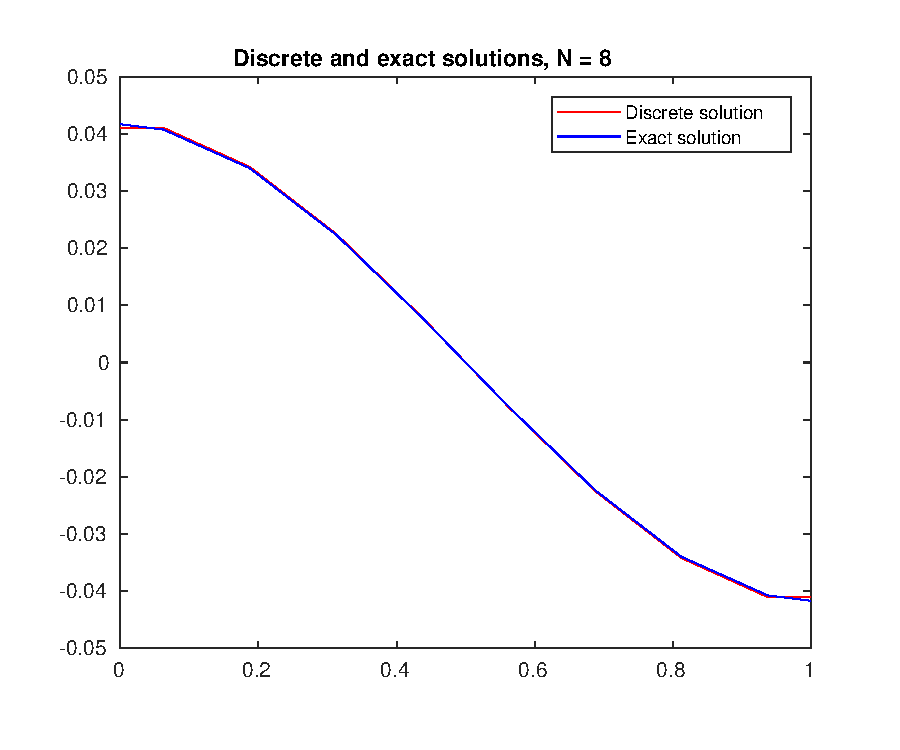
\includegraphics[width=10.5cm]{fig_neumann_result_G1_CP1_I1_N8_M6_C1}
\caption{Neumann result, $N=8$, Case 1.}
\end{figure}
\begin{figure}[H]
\centering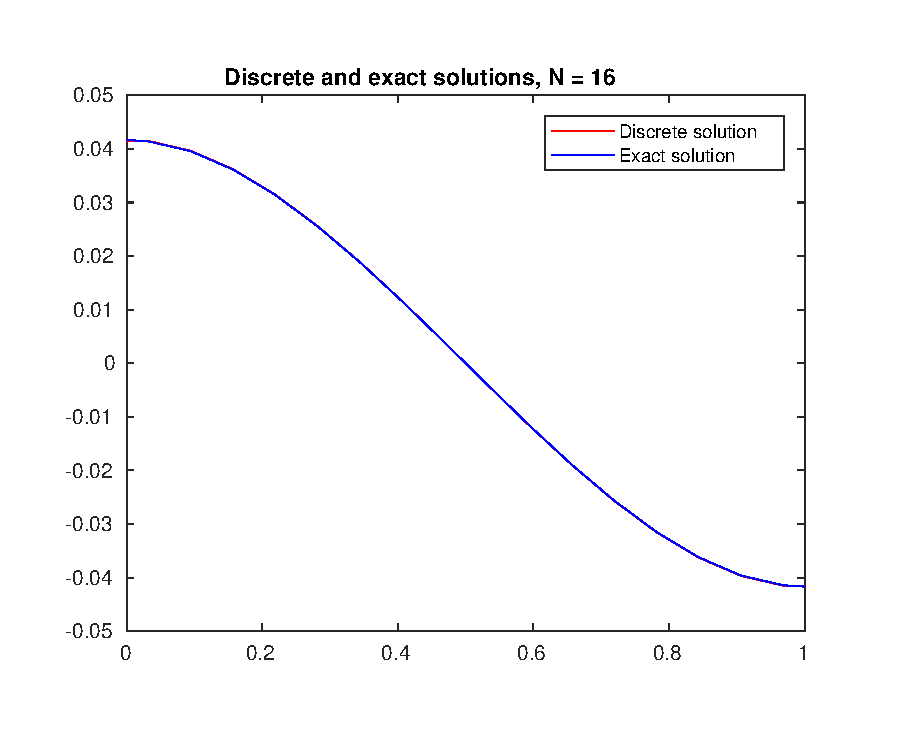
\includegraphics[width=10.5cm]{fig_neumann_result_G1_CP1_I1_N16_M6_C1}
\caption{Neumann result, $N=16$, Case 1.}
\end{figure}
\begin{figure}[H]
\centering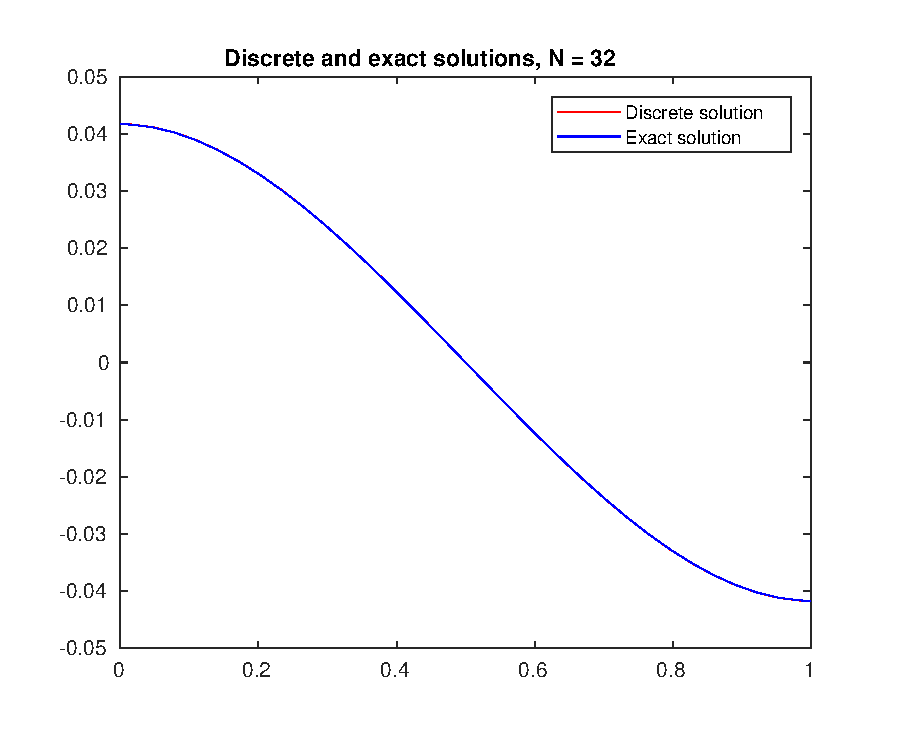
\includegraphics[width=10.5cm]{fig_neumann_result_G1_CP1_I1_N32_M6_C1}
\caption{Neumann result, $N=32$, Case 1.}
\end{figure}
\begin{figure}[H]
\centering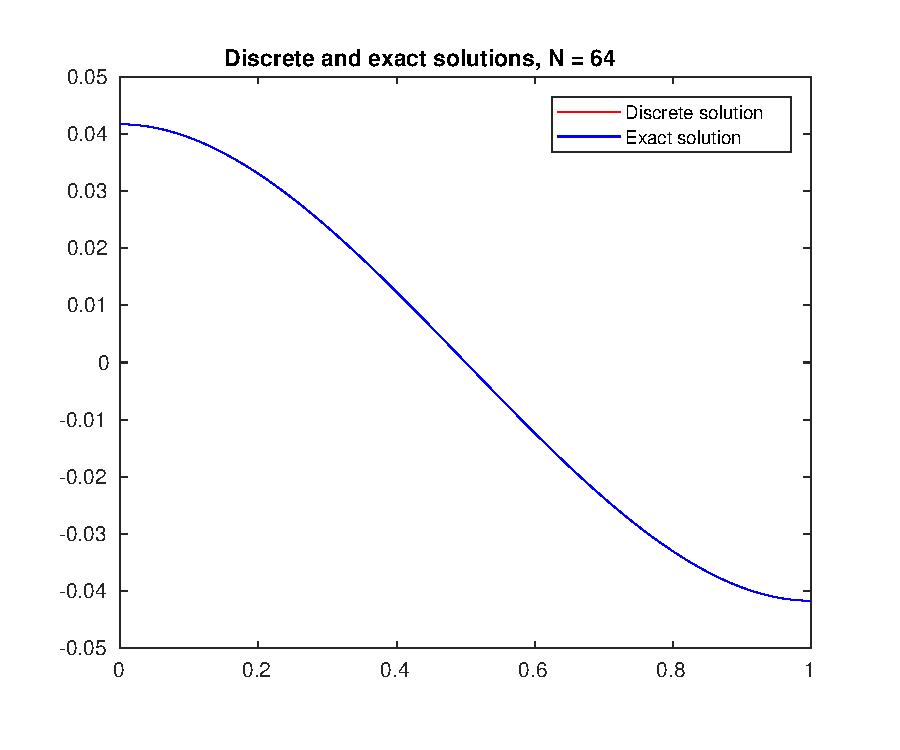
\includegraphics[width=10.5cm]{fig_neumann_result_G1_CP1_I1_N64_M6_C1}
\caption{Neumann result, $N=64$, Case 1.}
\end{figure}
\begin{figure}[H]
\centering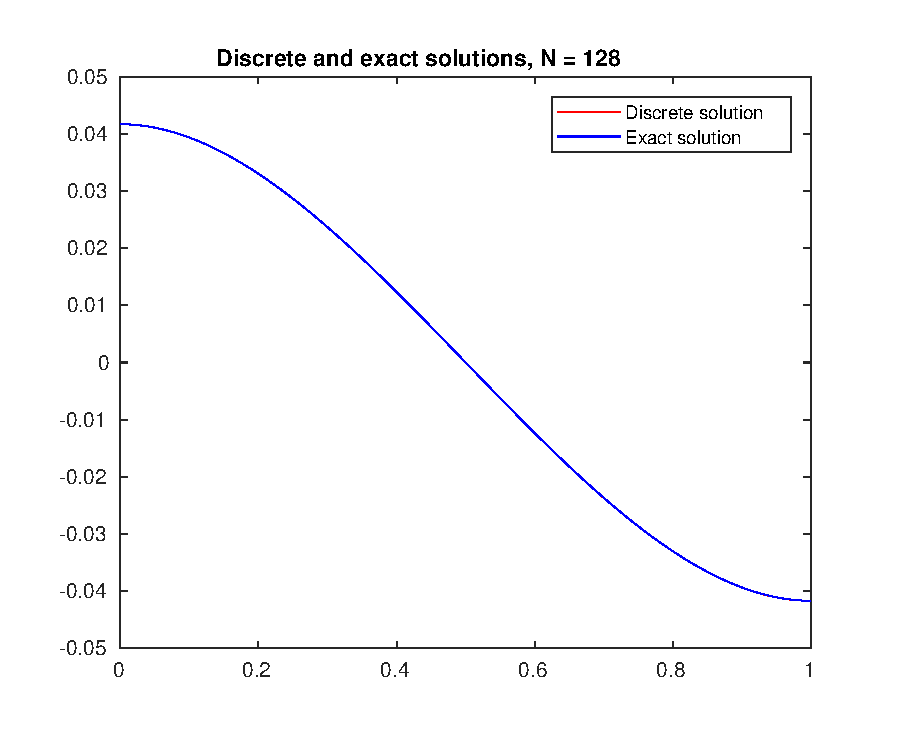
\includegraphics[width=10.5cm]{fig_neumann_result_G1_CP1_I1_N128_M6_C1}
\caption{Neumann result, $N=128$, Case 1.}
\end{figure}
\newpage
\noindent
\textsc{Case 2.}
\begin{figure}[H]
\centering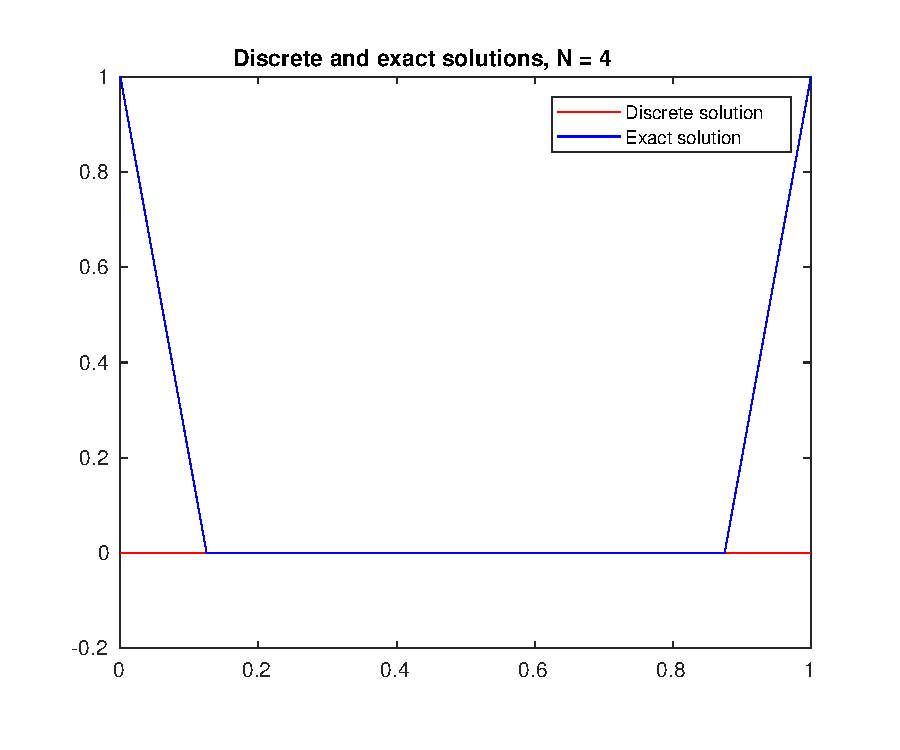
\includegraphics[width=10.5cm]{fig_neumann_result_G1_CP1_I1_N4_M6_C2}
\caption{Neumann result, $N=4$, Case 2.}
\end{figure}
\begin{figure}[H]
\centering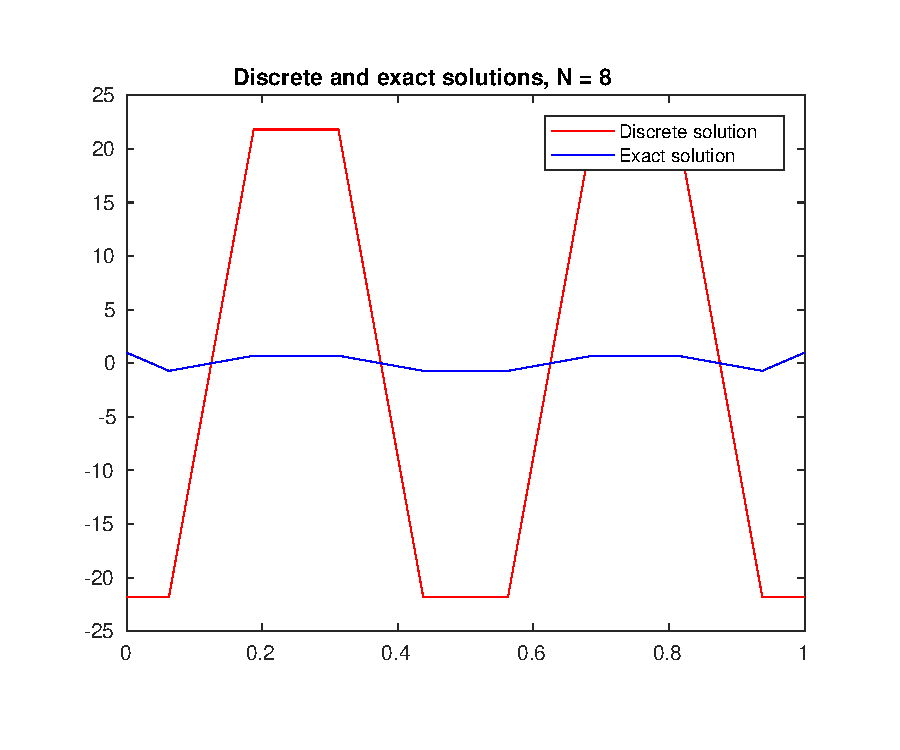
\includegraphics[width=10.5cm]{fig_neumann_result_G1_CP1_I1_N8_M6_C2}
\caption{Neumann result, $N=8$, Case 2.}
\end{figure}
\begin{figure}[H]
\centering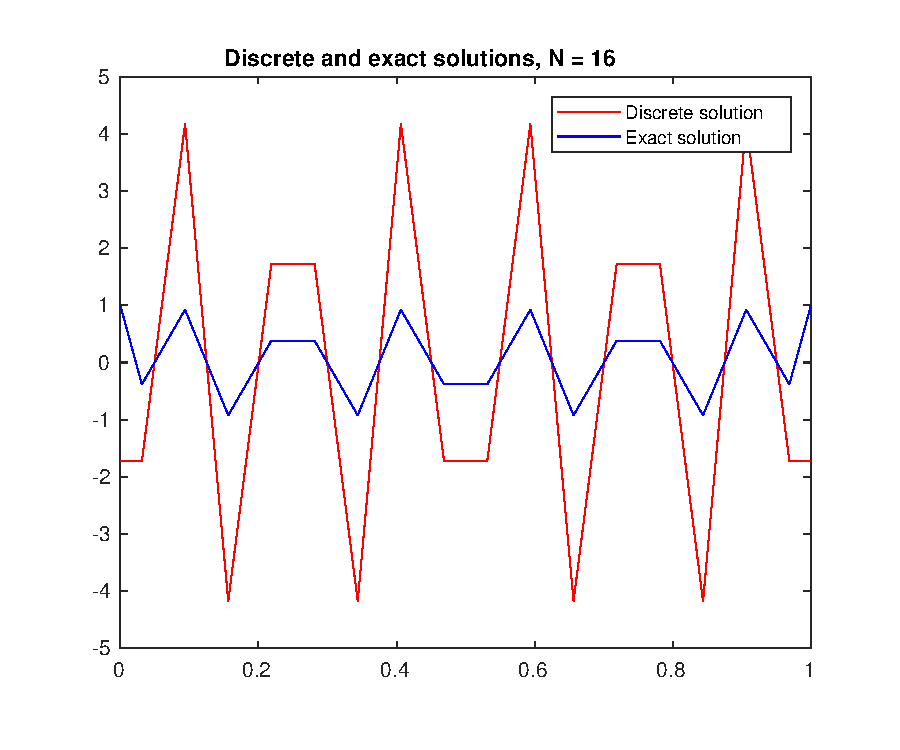
\includegraphics[width=10.5cm]{fig_neumann_result_G1_CP1_I1_N16_M6_C2}
\caption{Neumann result, $N=16$, Case 2.}
\end{figure}
\begin{figure}[H]
\centering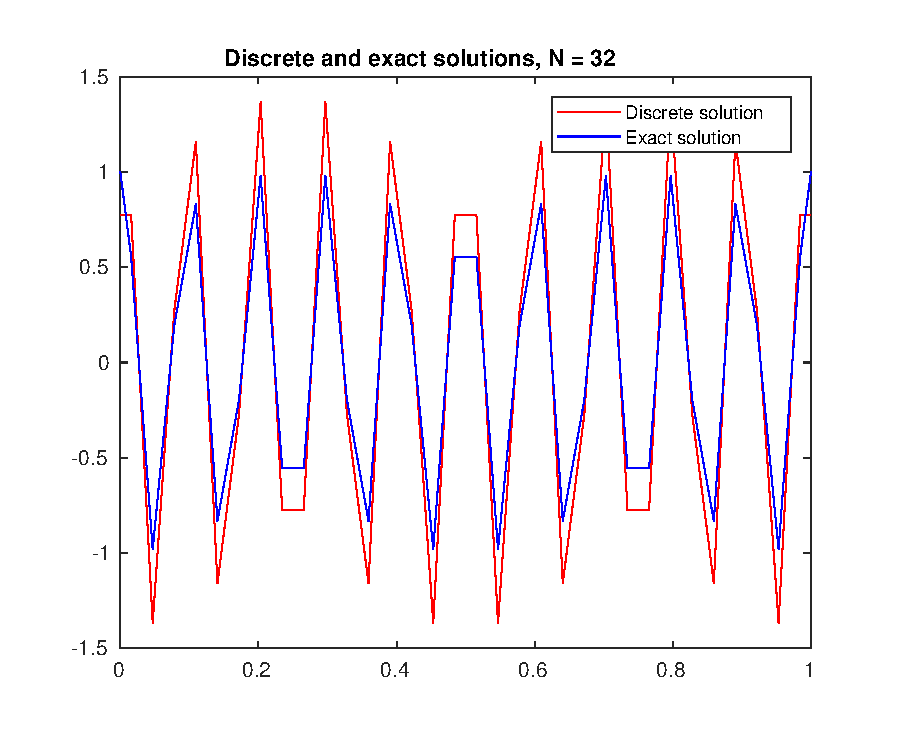
\includegraphics[width=10.5cm]{fig_neumann_result_G1_CP1_I1_N32_M6_C2}
\caption{Neumann result, $N=32$, Case 2.}
\end{figure}
\begin{figure}[H]
\centering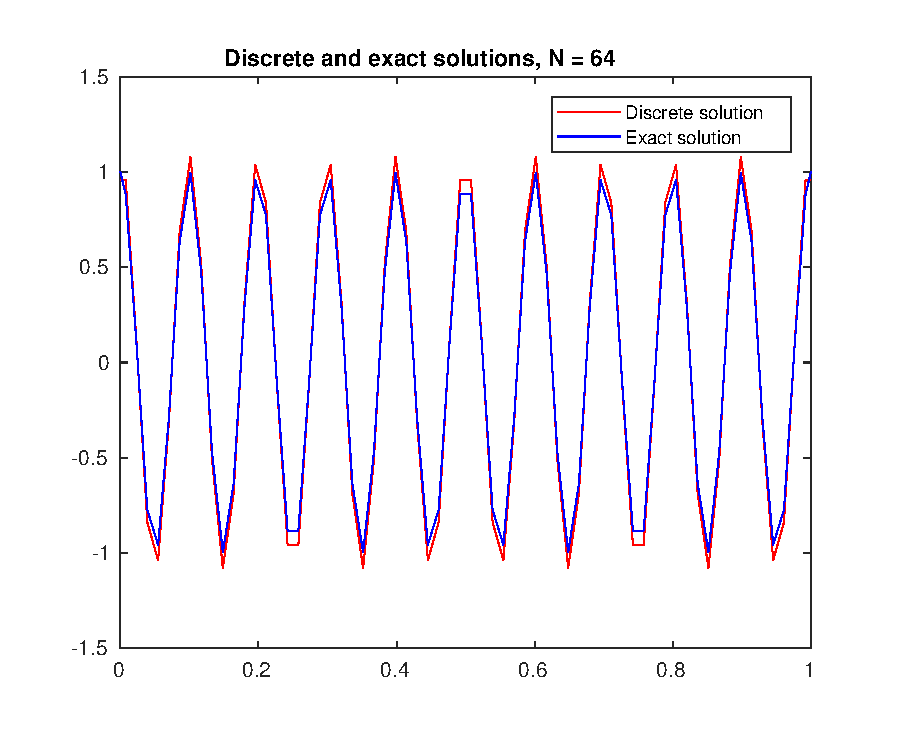
\includegraphics[width=10.5cm]{fig_neumann_result_G1_CP1_I1_N64_M6_C2}
\caption{Neumann result, $N=64$, Case 2.}
\end{figure}
\begin{figure}[H]
\centering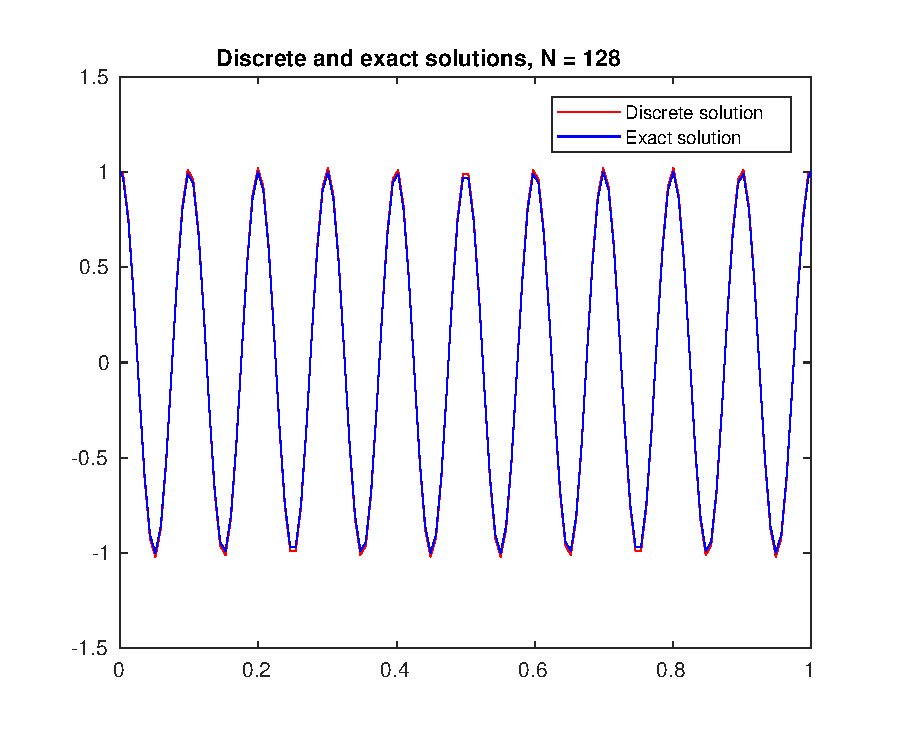
\includegraphics[width=10.5cm]{fig_neumann_result_G1_CP1_I1_N128_M6_C2}
\caption{Neumann result G1 CP1 I1 N128 M9 C2}
\end{figure}
\begin{figure}[H]
\centering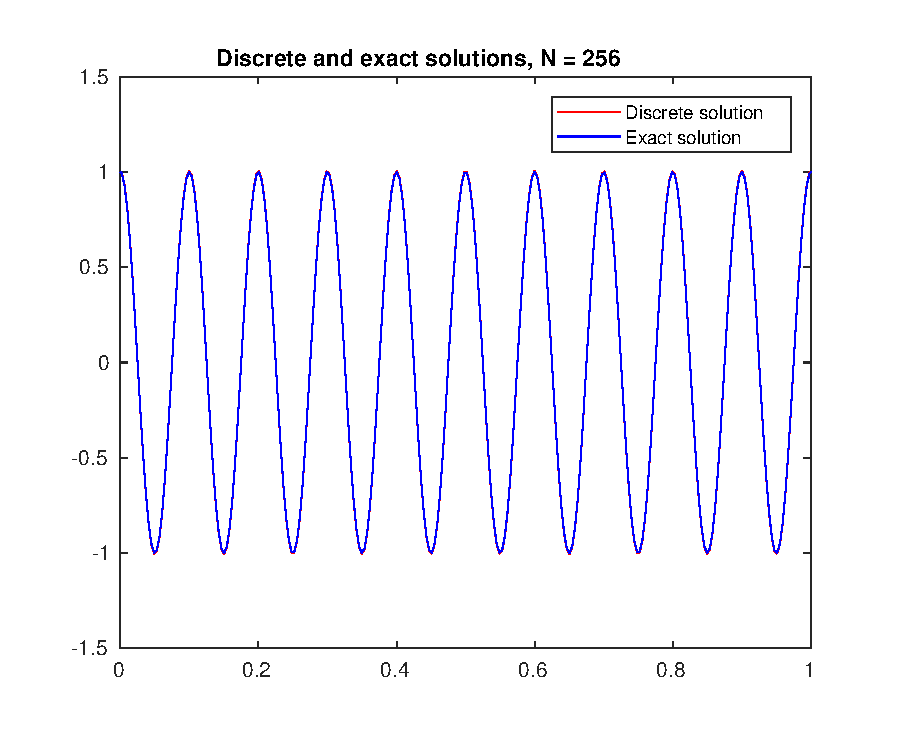
\includegraphics[width=10.5cm]{fig_neumann_result_G1_CP1_I1_N256_M9_C2}
\caption{Neumann result, $N=256$, Case 2.}
\end{figure}
\begin{figure}[H]
\centering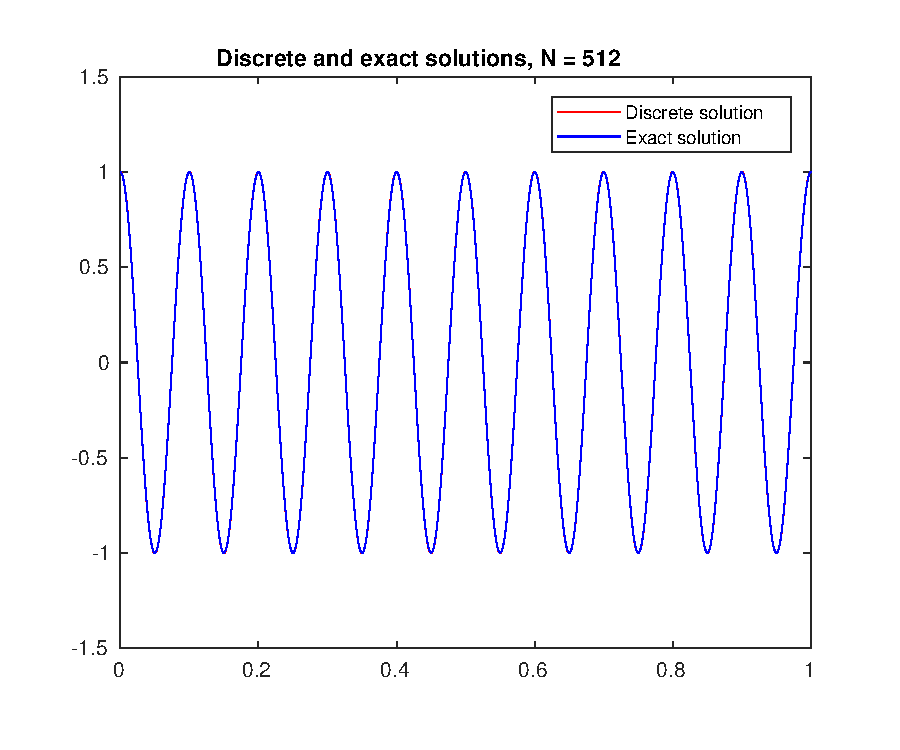
\includegraphics[width=10.5cm]{fig_neumann_result_G1_CP1_I1_N512_M9_C2}
\caption{Neumann result, $N=512$, Case 2.}
\end{figure}
\begin{figure}[H]
\centering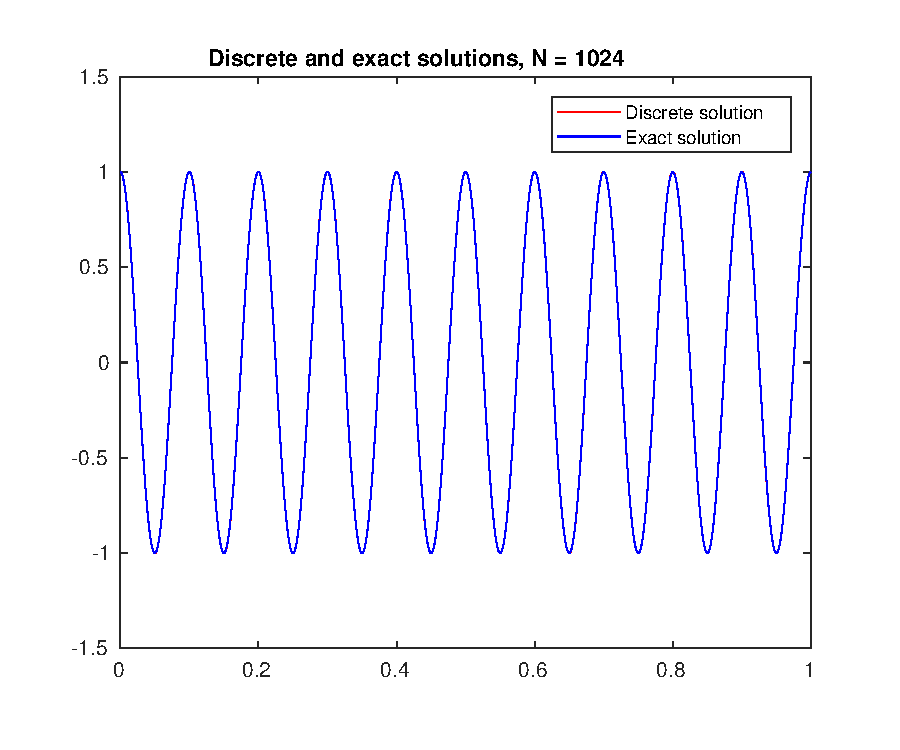
\includegraphics[width=10.5cm]{fig_neumann_result_G1_CP1_I1_N1024_M9_C2}
\caption{Neumann result, $N=1024$, Case 2.}
\end{figure}
\subsubsection{Errors}
\textsc{Case 1.}
\begin{table}[H]
\centering
\begin{tabu}{|c|c|c|}
\hline
			$N$	&  $\lVert u_{discrete}-u_{exact}\rVert_{L^2}$& $\lVert u_{discrete}-u_{exact}\rVert_{H^1}$ \\\hline
			4	& 7.278867e-04 & 1.449939e-02 \\\hline
			8	& 1.864655e-04 & 5.329006e-03 \\\hline
			16	& 4.689303e-05 & 1.918917e-03 \\\hline
			32	& 1.174048e-05 & 6.845135e-04 \\\hline
			64	& 2.936197e-06 & 2.430787e-04 \\\hline
			128	& 7.341164e-07 & 8.612922e-05 \\\hline
\end{tabu}
\caption{Error table}
\end{table}
\newpage
\noindent
\textsc{Case 2.}
\begin{table}[H]
\centering
\begin{tabu}{|c|c|c|}
\hline
			$N$	&  $\lVert u_{discrete}-u_{exact}\rVert_{L^2}$& $\lVert u_{discrete}-u_{exact}\rVert_{H^1}$ \\\hline
			4	& 3.446145e-13 & 4.000000e+00 \\\hline
			8	& 2.110184e+01 & 2.389353e+02 \\\hline
			16	& 2.486740e+00 & 7.434583e+01 \\\hline
			32	& 2.787005e-01 & 1.565996e+01 \\\hline
			64	& 5.963946e-02 & 4.064360e+00 \\\hline
			128	& 1.437125e-02 & 1.122033e+00 \\\hline
			256	& 3.560351e-03 & 3.281879e-01 \\\hline
			512	& 8.880771e-04 & 1.017972e-01 \\\hline
			1024	& 2.218939e-04 & 3.318688e-02 \\\hline
\end{tabu}
\caption{Error table}
\end{table}
\subsubsection{Convergence rate}
\textsc{Case 1.}
\begin{figure}[H]
\centering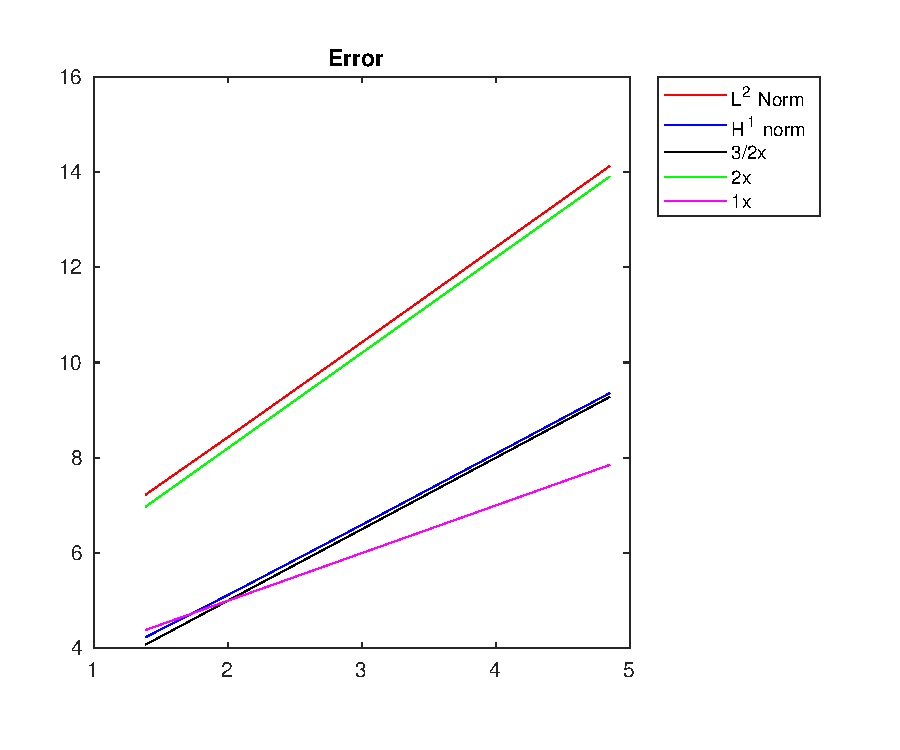
\includegraphics[width=13.5cm]{fig_neumann_error_G1_CP1_I1_M6_C1}
\caption{Neumann error, Case 1.}
\end{figure}
\newpage
\noindent
\textsc{Case 2.}
\begin{figure}[H]
\centering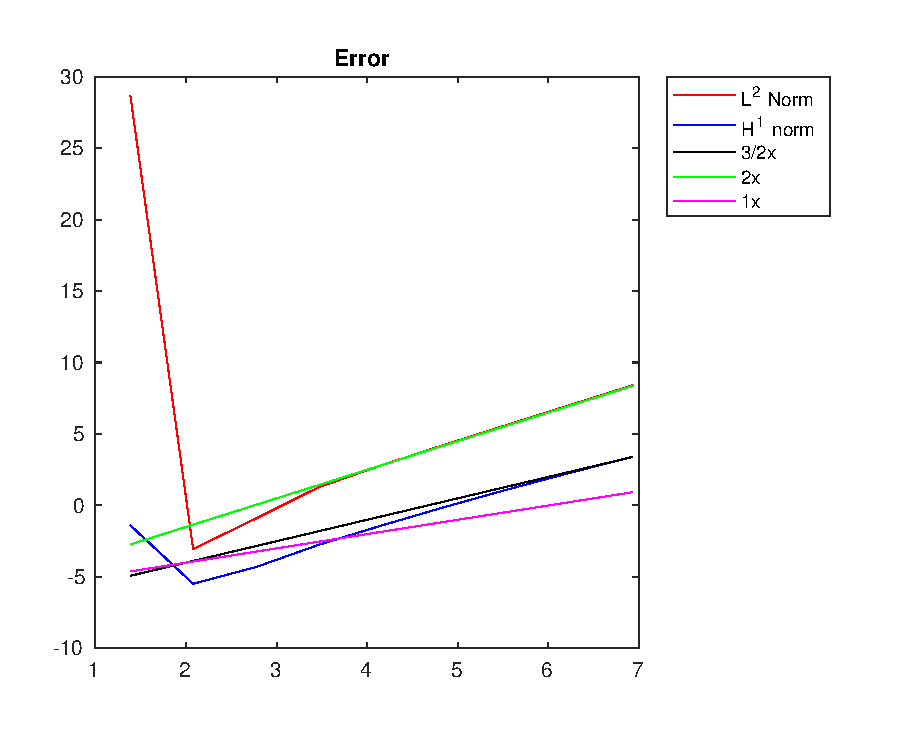
\includegraphics[width=13.5cm]{fig_neumann_error_G1_CP1_I1_M9_C2}
\caption{Neumann error, Case 2.}
\end{figure}
\noindent\textbf{Remark 8.1.} In both case 1 and 2, the method appears to have convergence rate of order $2$ in $L^2$ norm and order $\frac{3}{2}$ in energy norm.

\subsection{Homogeneous Neumann boundary condition, singular grid, each control point is the midpoint of corresponding control volume, integration using midpoint rule}
Again, we will consider the grid 
\begin{align}
x_i=1-\cos\left(\frac{\pi i}{2(N+1)}\right)
\end{align}
in this section.
\newpage
\subsubsection{Errors}
\textsc{Case 1.}
\begin{table}[H]
\centering
\begin{tabu}{|c|c|c|}
\hline
			$N$	&  $\lVert u_{discrete}-u_{exact}\rVert_{L^2}$& $\lVert u_{discrete}-u_{exact}\rVert_{H^1}$ \\\hline
			4	& 4.300279e-03 & 2.361702e-02 \\\hline
			8	& 4.473365e-04 & 7.452580e-03 \\\hline
			16	& 7.886546e-05 & 2.530245e-03 \\\hline
			32	& 1.995312e-05 & 9.154423e-04 \\\hline
			64	& 5.129577e-06 & 3.310069e-0 \\\hline
			128	& 1.302358e-06 & 1.185516e-04 \\\hline
\end{tabu}
\caption{Error table.}
\end{table}
\noindent
\textsc{Case 2.}
\begin{table}[H]
\centering
\begin{tabu}{|c|c|c|}
\hline
			$N$	&  $\lVert u_{discrete}-u_{exact}\rVert_{L^2}$& $\lVert u_{discrete}-u_{exact}\rVert_{H^1}$ \\\hline
			4	& 2.518759e+02 & 8.229286e+02 \\\hline
			8	& 2.924364e+01 & 2.378888e+02 \\\hline
			16	& 9.888043e+01 & 3.764880e+02 \\\hline
			32	& 5.525841e-01 & 2.551420e+01 \\\hline
			64	& 1.099226e-01 & 6.825063e+00 \\\hline
			128	& 2.584269e-02 & 1.840590e+00 \\\hline
			256	& 6.388832e-03 & 5.196868e-01 \\\hline
			512	& 1.595856e-03 & 1.549021e-01 \\\hline
			1024	& 3.992680e-04 & 4.880113e-02 \\\hline
\end{tabu}
\caption{Error table.}
\end{table}
\newpage
\subsubsection{Convergence rate}
\textsc{Case 1.}
\begin{figure}[H]
\centering\includegraphics[width=13cm]{fig_neumann_error_G2_CP1_I1_M6_C1}
\caption{Neumann error, Case 1.}
\end{figure}
\newpage
\textsc{Case 2.}
\begin{figure}[H]
\centering\includegraphics[width=13cm]{fig_neumann_error_G1_CP1_I1_M9_C2}
\caption{Neumann error, Case 2.}
\end{figure}
\noindent\textbf{Remark 8.2.} In both case 1 and 2, the method appears to have convergence rate of order $2$ in $L^2$ norm and order $\frac{3}{2}$ in energy norm.
\section{Appendices}
\subsection{An Easy Change of Variables}
The purpose of this subsection is to transform an integral of the form $\int_a^b {f\left( x \right)dx} $ to an integral of the form $\int_c^d {\widetilde f\left( x \right)dx} $, where $a,b,c,d$ are given real numbers. 

To this end, we consider an arbitrary mapping $S$ for which $S:\left[ {a,b} \right] \mapsto \left[ {c,d} \right]$. There are a lot of mappings $S$ satisfying this requirement. For simplicity, we should choose the following linear mapping
\begin{align}
y=S\left( x \right) = \frac{{d - c}}{{b - a}}x + \frac{{bc - ad}}{{b - a}},\hspace{0.2cm}\forall x \in \left[ {a,b} \right]
\end{align}
and the inverse mapping of $S$ is given by
\begin{align}
x = {S^{ - 1}}\left( y \right) = \frac{{b - a}}{{d - c}}y + \frac{{ad - bc}}{{d - c}},\hspace{0.2cm}\forall y \in \left[ {c,d} \right]
\end{align}
Then, we can use the change of variables $y=S\left(x\right)$ straightforward. 
\begin{align}
\label{6.3}
\int_a^b {f\left( x \right)dx}  = \int_c^d {f\left( {{S^{ - 1}}\left( y \right)} \right)\frac{{b - a}}{{d - c}}dy} 
\end{align}
Put 
\begin{align}
\widetilde f\left( y \right) = \frac{{b - a}}{{d - c}}f\left( {{S^{ - 1}}\left( y \right)} \right),\hspace{0.2cm}\forall y \in \left[ {c,d} \right]
\end{align}
We can rewritten \eqref{6.3} as
\begin{align}
\int_a^b {f\left( x \right)dx}  = \int_c^d {\widetilde f\left( x \right)dx} 
\end{align}
as required. \hfill $\square$
\subsection{Some Useful Inequalities}
\textbf{Proposition 9.1.} \textit{Let $a,b,c,d$ be nonnegative real numbers. The following inequality holds}
\begin{align}
\label{6.6}
{\left( {\sqrt {ab}  + \sqrt {cd} } \right)^2} \le \left( {a + c} \right)\left( {b + d} \right)
\end{align}
\textsc{Proof.} It is a direct consequence of Cauchy-Schwarz inequality. Indeed,
\begin{align}
{\left( {\sqrt {ab}  + \sqrt {cd} } \right)^2} &= ab + cd + 2\sqrt {abcd} \\
& \le ab + cd + bc + ad\\
& = \left( {a + c} \right)\left( {b + d} \right)
\end{align}
The equality occurs if and only if $bc=ad$. \hfill $\square$\\
\\
\\
\\
\begin{center}
\textsc{The End}
\end{center}
\newpage
\printindex
\newpage
\begin{thebibliography}{999}
\bibitem {1} Robert Eymard, Thierry Gallou\"{e}t, Rapha\`{e}le Herbin, \textit{Finite Volume Methods}, October 2006.
\bibitem {2} Anh Ha Le, Huong Lan Tran, \textit{Finite Volume Method in 1D}, University of Sciences, March 12, 2014.
\bibitem {3} \url{https://en.wikipedia.org/wiki/Cauchy%E2%80%93Schwarz_inequality}
\end{thebibliography}
\end{document}